\documentclass{article}

\usepackage{fancyhdr} % Required for custom headers
\usepackage{lastpage} % Required to determine the last page for the footer
\usepackage{extramarks} % Required for headers and footers
\usepackage[usenames,dvipsnames]{color} % Required for custom colors
\usepackage{graphicx} % Required to insert images
\usepackage{listings} % Required for insertion of code
\usepackage{courier} % Required for the courier font
\usepackage{lipsum} % Used for inserting dummy 'Lorem ipsum' text into the template
\usepackage{titling}
\usepackage{booktabs}
\usepackage{tikz}
\usepackage{calc}
\def\checkmark{\tikz\fill[scale=0.4](0,.35) -- (.25,0) -- (1,.7) -- (.25,.15) -- cycle;} 
\def\scalecheck{\resizebox{\widthof{\checkmark}*\ratio{\widthof{x}}{\widthof{\normalsize x}}}{!}{\checkmark}}
%\usepackage{hyperref}
\topmargin=-0.0in
\evensidemargin=0in
\oddsidemargin=0in
\textwidth=6.5in
\textheight=9.0in
\headsep=0.25in

\newcommand{\hmwkTitle}{Shape Categorization\\Final Report} % Assignment title
\newcommand{\hmwkClass}{Computer Vision} % Course/class Class/lecture time
\newcommand{\hmwkClassInstructor}{Prof. Dr.-Ing. Rainer Herpers} % Teacher/lecturer
\newcommand{\hmwkimage}{\centering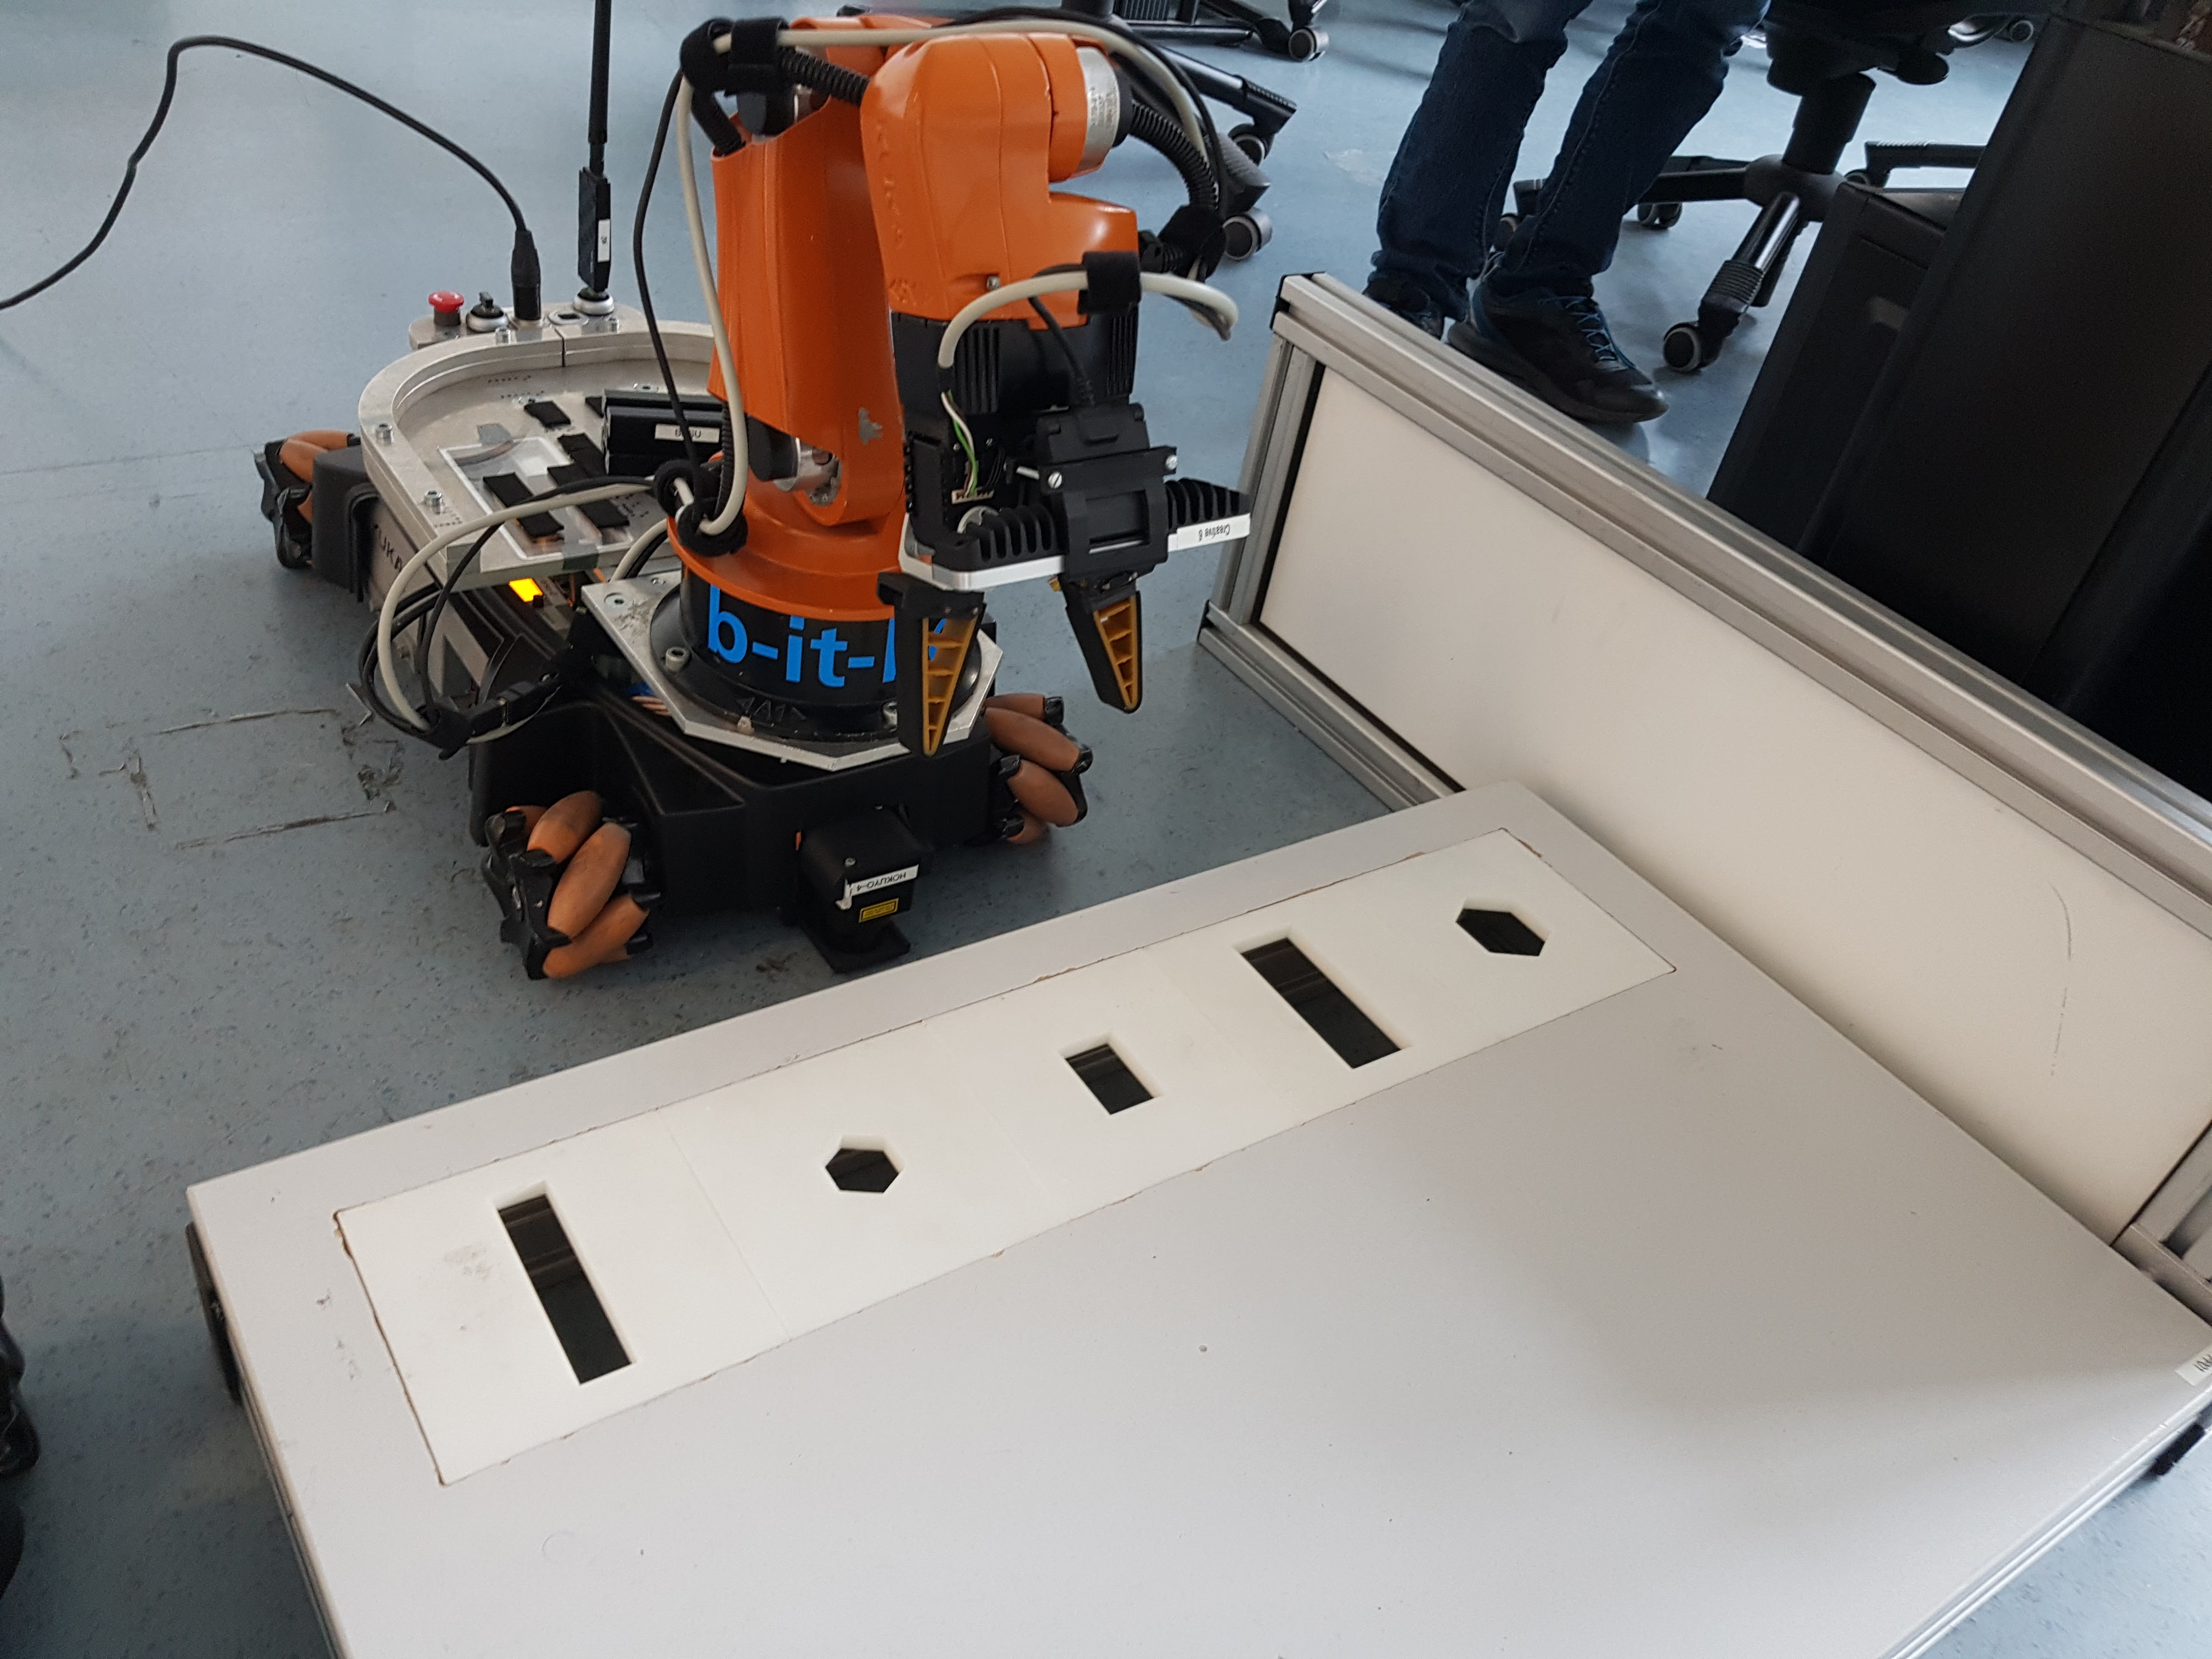
\includegraphics[draft=false, scale = 0.075]{images/FrontPicture.jpg}}
\newcommand{\hmwkAuthorName}{Senthilkumar Sockalingam Kathiresan} % Your name
\newcommand{\hmwksecondauthor}{Yannick Weitz}
\newcommand{\hmwkfirstmat}{Matrikel Nr. 9030382}
\newcommand{\hmwksecondmat}{Matrikel Nr. 9030385}

%----------------------------------------------------------------------------------------
%	TITLE PAGE
%----------------------------------------------------------------------------------------


\title{
\vspace{2in}
\textmd{\textbf{\hmwkClass:\ \\ \hmwkTitle}}\\
\vspace{0.1in}\large{\hmwkClassInstructor\ }
\vspace{3in}
}

\author{\textbf{\hmwkAuthorName}, \hmwkfirstmat\\ \textbf{\hmwksecondauthor}, \hmwksecondmat}
\date{} % Insert date here if you want it to appear below your name

\begin{document}
\begin{titlepage}
\hmwkimage\\
\vspace{1in}
\textmd{\Huge\textbf{\hmwkClass:\ \\ \hmwkTitle}}\\
\vspace{0.1in}\large{\hmwkClassInstructor\ }
\vspace{3in}\\
\theauthor\
\thispagestyle{empty}
\end{titlepage}


\setcounter{page}{1}

\tableofcontents

\newpage

%----------------------------------------------------------------------------------------
%	INTRODUCTION
%----------------------------------------------------------------------------------------

\section{Introduction}

 The computer vision project "Shape Recognition" is based on a task "Precision Placement Test" given in the robocup@work competition rulebook. According to this task, a robot should be able to fit a three-dimensional object (fig) in a two-dimensional cavity tile (). The tiles will be placed in the work table called PPT (Precision Placement Test) platform (Figure\ref{fig:PPT}). To succeed at this task, the robot should have robust perception and manipulation capabilities.
 
	The project "Shape Recognition" deals with the perception requirement for the precision placement task.
By this project, the robot should be able to find the objects and their orientation that will fit in the cavities of the tiles, given the image of the PPT platform.

	A series of digital image filters such as adaptive thresholding, canny edge filter, etc.,  are applied to the input image. From the processed image the tiles are extracted. The extracted cavity tiles are then cropped from the original image. Homography is done over the cropped images to get the top view of the cavity tiles. This extracted top view of the cavity tiles is then compared with the cavity tiles stored in the database to identify the best match. In addition to the images stored in the database, details on the orientation and the object fitting into the cavity are stored.

%The Task that should be solved by this Computer Vision project is based on a Task taken from the Robocup@Work rulebook. The youBot should be able to fit a 3 dimensional piece into the correct 2 dimensional cavity.\\
%In order to fit the part into the cavity, the correct cavity has to be determined first. The whole task is testing the perception as well as the manipulation ability of the youbot.\\
%As given by the rule book of the Robocup@work:

%\begin{quote}
%
%single robot is used.  The robot is placed by the team freely within the arena.  The
%objective of the task is to pick the objects which are placed on one service area and make a
%precise-placement in the corresponding cavity at the service area with the special PPT platform
%(an example configuration is illustrated in Figure
%3.2).
%The task consists of multiple grasp and place operations, possibly with base movement in be-
%tween, which will, however, be short.  The task is finished once the objects are picked up and
%placed in the corresponding cavities or when the time foreseen for the run ends.  Note that the
%placement of the object in the cavity is finished when the object is fallen into the cavity (i.e.  at
%least some part of the object has to touch ground floor underneath the cavity).
%All objects to be transported in a run of a team and the corresponding cavities share the same
%orientation, either horizontal or vertical.  This may vary between different teams and different
%runs.[1]\\
%
%\end{quote}

%----------------------------------------------------------------------------------------
%	Material and Methods
%----------------------------------------------------------------------------------------

\section{Material and methods}

\subsection{Description of the setup}
\textbf{From the rule book:}
\begin{quote}
\begin{itemize}
\item A single youBot is used. 
\item The robot is placed by the team freely within the arena. 
\item The objective of the task is to pick the objects which are placed on one service area and make a
precise-placement in the corresponding cavity at the service area with the special PPT platform
\begin{figure}[h!]
\centering
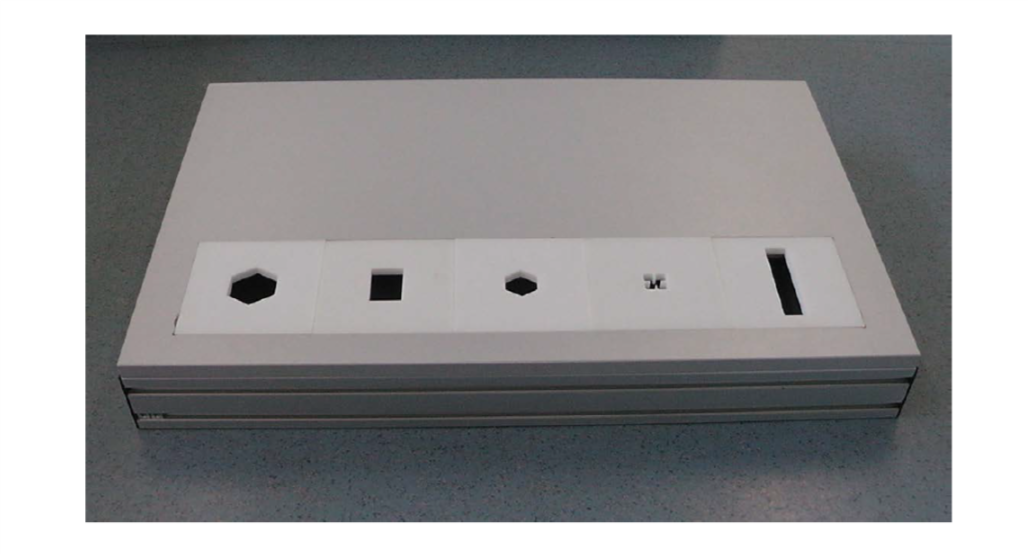
\includegraphics[scale=0.5]{images/PPT_Platform.png}
\caption{The PPT platform including five cavity tiles}
\label{fig:PPT}
\end{figure}
(an example configuration is illustrated in Figure
\ref{fig:PPT}).
\item The task consists of multiple grasp and place operations, possibly with short base movement in between. 
\item The task is finished once the objects are picked up and
placed in the corresponding cavities or when the time foreseen for the run ends.
\item  Note that the
placement of the object in the cavity is finished when the object is fallen into the cavity (i.e.  at
least some part of the object has to touch ground floor underneath the cavity).
\item All objects to be transported in a run of a team and the corresponding cavities share the same
orientation, either horizontal or vertical.  This may vary between different teams and different
runs.[1]
\end{itemize}

\end{quote}

\subsection{PPT platform details: }

\begin{quote}
\begin{itemize}
\item The color of the PPT platform is a light grey.
\item There will always be five tiles (Figure \ref{fig:PPT}) 
\item There will be no gap between the tiles (Figure \ref{fig:PPT})
\end{itemize}
\end{quote}




\subsection{Object details:}

\begin{enumerate}
\item Large aluminium profile
\item Small aluminium profile
\item Large nut
\item Small nut
\item Screw
\item Cylinder 
\end{enumerate}

\begin{figure}[h!]
\begin{center}
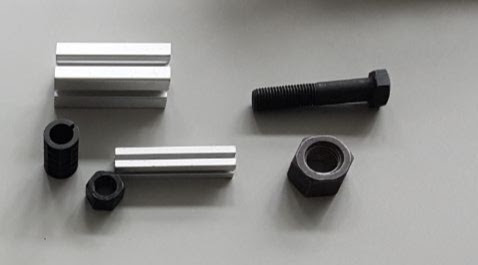
\includegraphics[scale=0.5]{images/AllParts.jpg}
\end{center}
\caption{six objects which has to be placed in the cavity tiles \cite{second} }
\end{figure}

\subsection{Cavity tiles details:}
\begin{itemize}
\item There are 11 tiles that will be used in the competition
\item Each tile measures 14 x 14 cm 
\item The color of the tile is close to white
\item The material is 3D printed
\end{itemize}
\begin{figure}[h!]
\centering
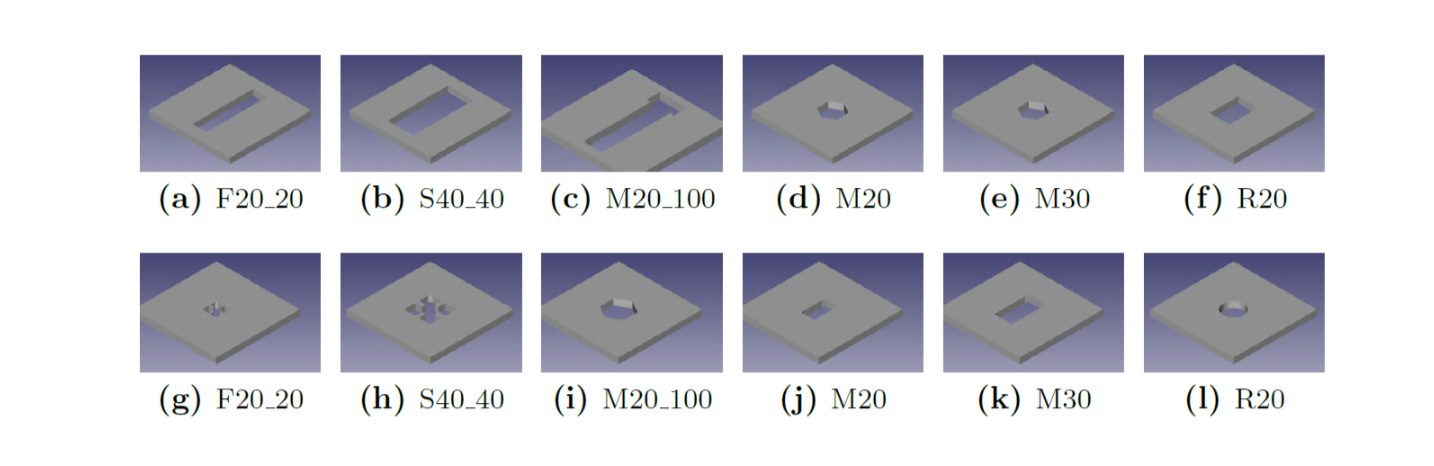
\includegraphics[scale=1.0]{images/AllTiles.png}
\caption{Cavity tiles for the objects}
\label{fig:tiles}
\end{figure}


\subsection{Camera details:}
\begin{itemize}
\item Camera model fixed to the robot is \textbf{asus xtion pro live} (Figure \ref{fig:camera} )
\item \textbf{Intrinsic parameters}




\begin{itemize}
\item height: 480
\item width: 640
\item distortion model: plumb bob
\item D: [0.0, 0.0, 0.0, 0.0, 0.0]
\item K: [570.3422241210938, 0.0, 319.5, 0.0, 570.3422241210938, 239.5, 0.0, 0.0, 1.0]
\item R: [1.0, 0.0, 0.0, 0.0, 1.0, 0.0, 0.0, 0.0, 1.0]
\item P: [570.3422241210938, 0.0, 319.5, 0.0, 0.0, 570.3422241210938, 239.5, 0.0, 0.0, 0.0, 1.0, 0.0]
\item binning x: 0
\item binning y: 0
\item roi:
\item x offset: 0
\item y offset: 0
\item height: 0
\item width: 0
\item do rectify: False
\end{itemize} 
\end{itemize}

\begin{figure}[h!]
\centering
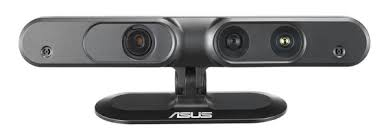
\includegraphics[scale=0.5]{images/camera.jpeg}
\caption{Asus xtion pro live}
\label{fig:camera}
\end{figure}


\newpage


\textbf{Prerequisites}\\

For the precision and placement test the youBot will get the command to pick up a particular part from a toolbox, from the referee unit, and then drive back to the table, where the cavities are stored. This is where the project begins. The camera of the youBot is pointing at the table. Five out of twelve plates will be placed in a cavities inside the table, arranged in a row (fig. \ref{fig:row}). The background of the cavities inside the tiles will thus be dark and the full tile will always be visible. The tiles themselves have a nearly white color and will be produced by a 3D printer. The size is fixed to $14cm^2$, with a thickness of  $1cm$ .\\
The object, that the youBot is holding is already recognized and known to the bot. There are 5 different objects available.\\
The cavities are always centered in the middle of the tile and will only correspond to only one particular orientation of the object.\\
The youBot is using a asus xtion pro live for this task. The camera will be positioned in front of the tiles, with different possible angles, always capturing all five tiles. \\
There will be no additional light source attached to the youBot, so shadows are possible.\\

\begin{figure}[h!]
\centering
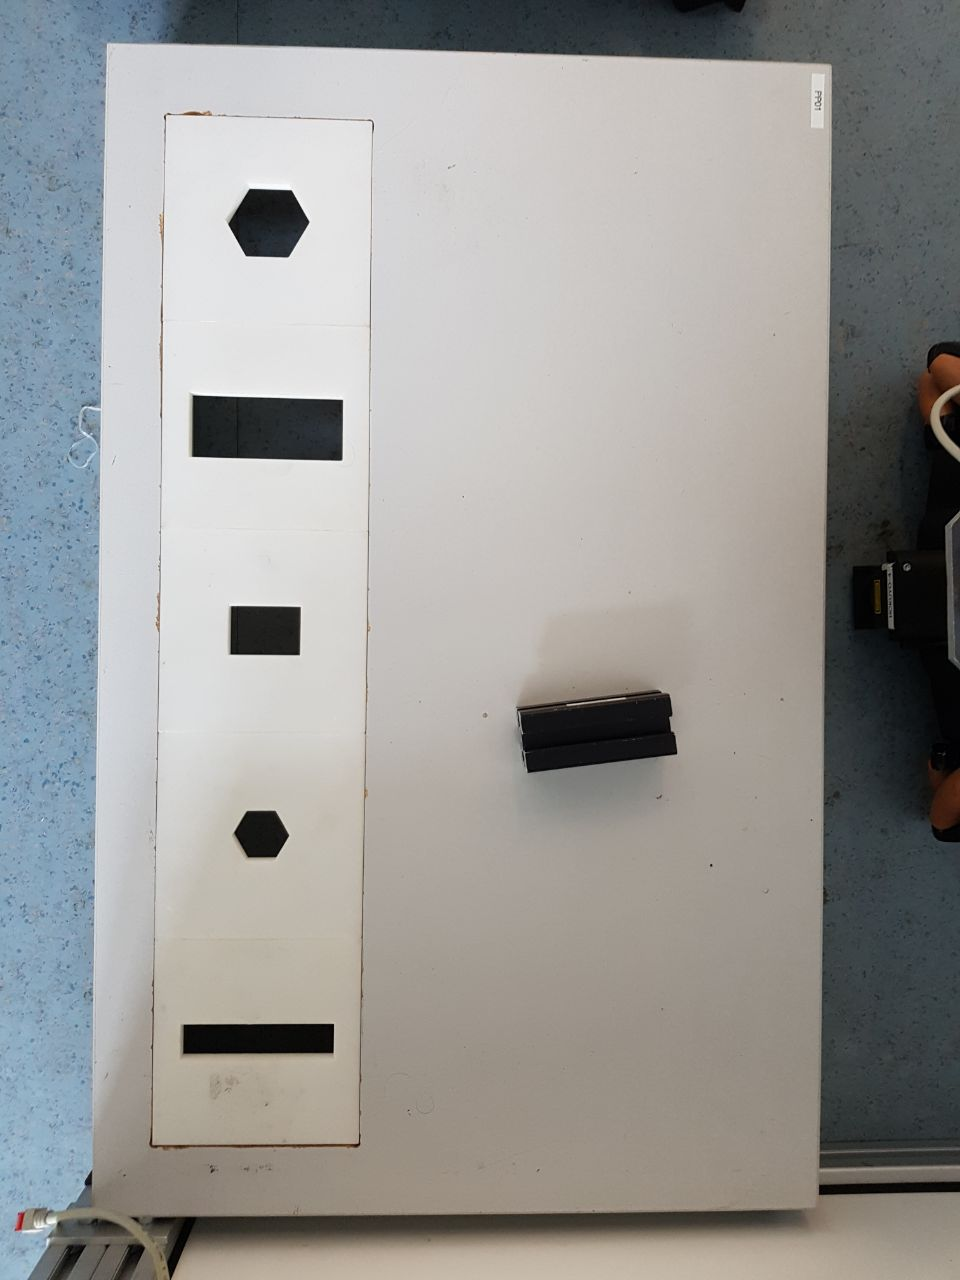
\includegraphics[scale=0.15,angle=270]{images/5tiles.jpeg}
\caption{Example of a set of five tiles arranged like they will be in the Robocup@Work competition.}
\label{fig:row}
\end{figure}




\section{Approach}

%\textbf{General Approach}

As a preprocessing step the image input has to be normalized. Since it can't be assumed that the youBot will always provide a 90$^\circ$ top-down view of the tiles, the input image should should be transformed using homography. The new image after this step should only show an approximate of what the row of tiles would look like from the 90$^\circ$ top-down view. The result will then be further decomposed into the single tiles.\\
To classify the extracted tiles, a comparison between the tiles and a database is performed. The database consists of example images showing all the tiles in all possible configurations.\\

The project is divided into three phases: 
\begin{enumerate}
\item Getting rid of Unnecessary information
\item Cavity tile extraction
\item Comparison
\end{enumerate}

\subsection{Getting rid of Unnecessary information}

In order to normalize the input image and rectify the row of tiles, the first step is to crop the image and get rid of unnecessary information (fig. \ref{fig:original}). \\
\begin{figure}[h!]
\centering
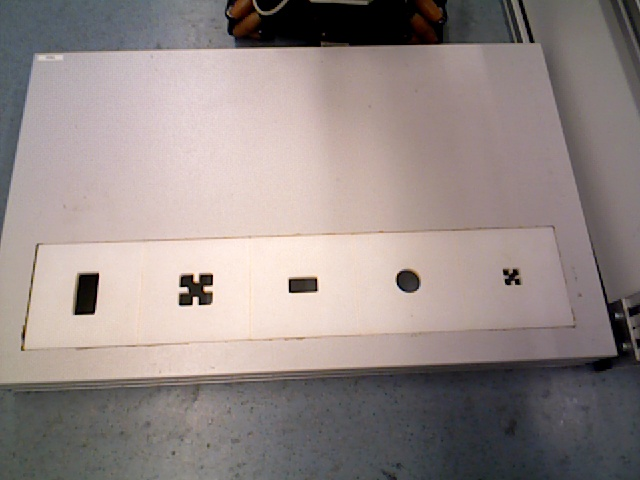
\includegraphics[scale=0.3]{images/frame01.jpg}
\caption{The Original image containing irrelevant information, like the table or small parts of the robot.}
\label{fig:original}
\end{figure}

\subsubsection*{Edge filter}
so at first the area that should be cropped has to be determined. Since the images are in general a lot brighter than the cavities, an edge filter is applied (fig. \ref{fig:edges}). Threshold and adaptive threshold have been tested but didn't deliver good results.\\
\begin{figure}[h!]
\centering
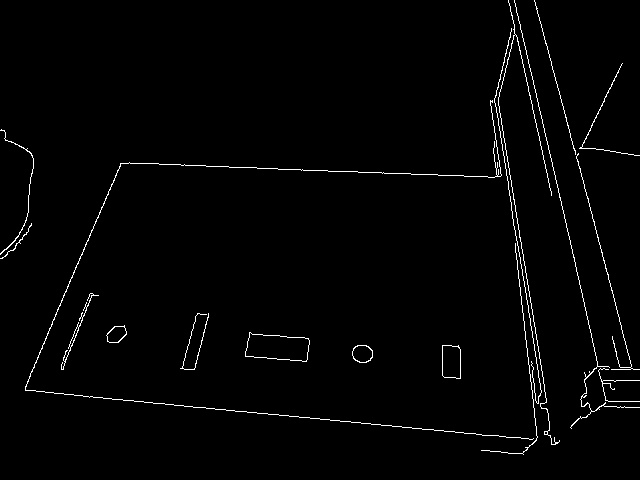
\includegraphics[scale=0.3]{images/edges.jpg}
\caption{The image after a canny edge filter has been applied.}
\label{fig:edges}
\end{figure}

\subsubsection*{Contour extraction}
Using the findContours method all contours of the preprocessed image are extracted and the pixel coordinates of the center points are stored (fig. \ref{fig:cavities}). Since all contours should lie in the middle of the tiles, the centers of the cavities should lie in a line consisting of five equally spaces points. \\
The first attempt to this problem was to use blobdetection in order to extract dark areas in the image. This method failed due to the multitude in cavity shapes and many other dark regions in the image. Also the datastructure of the blobs made it hard to enter the information. 
\begin{figure}[h!]
\centering
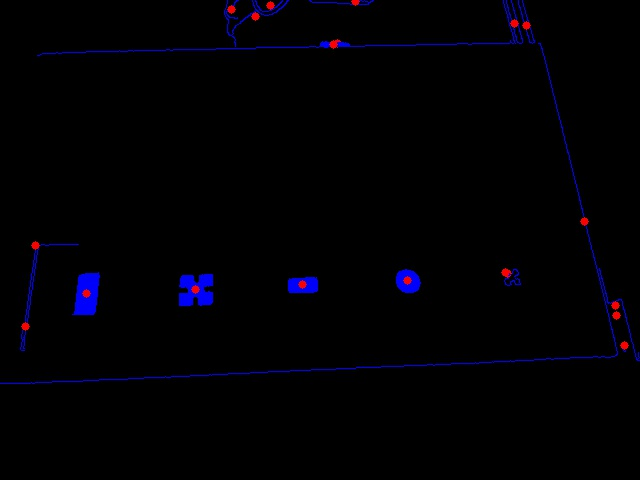
\includegraphics[scale=0.3]{images/cavitycontours.jpg}
\caption{All the extracted contours from the edge detection image.}
\label{fig:cavities}
\end{figure}

\subsubsection*{Finding the center of the cavities}
To find the five points that correspond to these centers, a line is drawn between all extracted centers from substep one. From all the lines where at least five points lie closely on the same line, the one is chosen where the error between the points and the line is the least (fig. \ref{fig:line}). This has proven to give the correct line for all tested images. Si-,
nce we search for the minimum distance, lines with five points are preferred over lines with more points, so by default lines with to many points get ruled out.\\
\begin{figure}[h!]
\centering
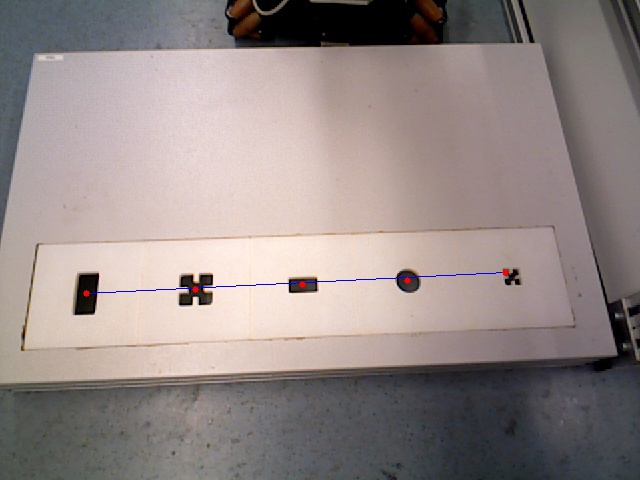
\includegraphics[scale=0.3]{images/line.jpg}
\caption{The five points that lie closest to a line have been extracted.}
\label{fig:line}
\end{figure}

\subsubsection*{Cropping out unnecessary information}
We know that all tiles have the same dimensions. Thus, the next step aims to find a correspondence between the pixels and the distance, or pixels per centimeter. The center points of the cavities are expected to lie in the center of the tile. It follows, that the distance between two neighboring centers is equal to $14cm$.Hence, The approximate pixel equivalent to $14cm$ is calculated by getting the mean distance between two neighboring tile centers.\\
Now the image can be cropped by using (fig. \ref{fig:cropped}):
\begin{equation}
cropped \, image = image[min(x)-\frac{\mu_{dist}}{2}:max(x)+\frac{\mu_{dist}}{2},min(y)-\frac{\mu_{dist}}{2}:max(y)+\frac{\mu_{dist}}{2}]
\end{equation}
Where:
\begin{quote}
$\frac{\mu_{dist}}{2}$ = Pixel per 7 Centimeter, plus some additional term to compensate the angular orientation of the five tiles\\
$min(x)$ = Minimum x value of all center points\\
$max(x)$ = Maximum x value of all center points\\
$min(y)$ = Minimum y value of all center points\\
$max(y)$ = Maximum y value of all center points\\
\end{quote}
\begin{figure}[h!]
\centering
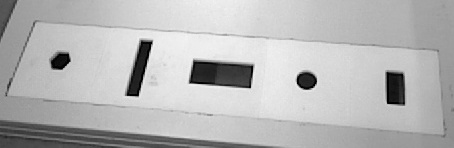
\includegraphics[scale=0.3]{images/cropped.jpg}
\caption{A lot of irrelevant information has been cropped out of the image.}
\label{fig:cropped}
\end{figure}

\subsection{Cavity tile extraction}

\subsubsection*{Corner detection}
To extract the corners of the five tile row, the adaptive threshold filter is applied to the cropped image, since this has proven to give a good differentiation between the five tile row and the background. Again the contours of the image are extracted, this time with a limitation of the area, that the contour should enclose (fig. \ref{fig:five}). The original approach used the goodFeaturesToTrack method. Because of the low resolution of the image the algorithm detects to many corners. to overcome this a method of choosing the correct corners is needed, but after multiple attempts, this approach was replaced by hough line transformation. The idea was to get the points, where the hough lines meet. However, the algorithm didn't extract good lines, that fit the sides of the contour and was thus discarded.\\

\begin{figure}[h!]
\centering
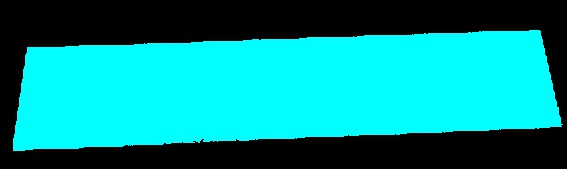
\includegraphics[scale=0.3]{images/5tiles.jpg}
\caption{The contour of the image that corresponds to the biggest area of the cropped image.}
\label{fig:five}
\end{figure}

The low resolution of the image makes it hard to extract the four corners immediately. The Harris corner detection is used to extract the four corner points, since these are a little misplaced the cornerSubPix method as described in [2] is used to extract the corners more precisely(fig. \ref{fig:points}).  \\

\begin{figure}[h!]
\centering

\includegraphics[scale=1]{images/Corners.jpg}
\caption{The two extracted corners are shown, red shows the Harris corner, while green shows the corner with sub pixel precision.}
\label{fig:points}
\end{figure}

\subsubsection*{Homography}
The four points are used to transform the perspective of the tiles to create and artificial top-down image containing only the five tiles (fig. \ref{fig:homograph}).\\
\begin{figure}[h!]
\centering
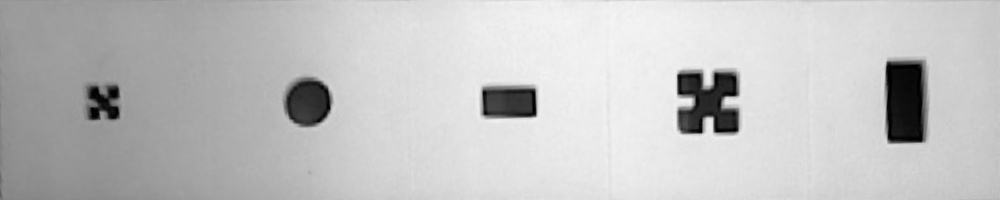
\includegraphics[scale=0.3]{images/homography.jpg}
\caption{An artifical top-down view of the five tiles.}
\label{fig:homograph}
\end{figure}

\subsubsection*{Cropping cavity tiles}

The resulting image is then divided into five equal parts and the images are stored (fig. \ref{fig:individ}).\\
\begin{figure}[h!]
\begin{minipage}{\textwidth}
\centering
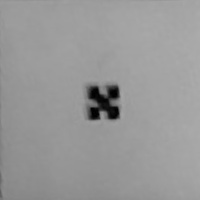
\includegraphics[scale=0.3]{images/tile0.jpg}
\hspace{0.1cm}
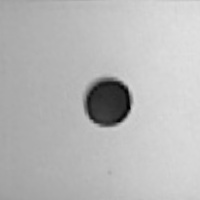
\includegraphics[scale=0.3]{images/tile1.jpg}
\hspace{0.1cm}
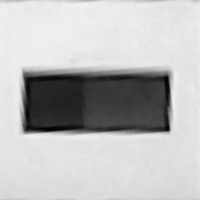
\includegraphics[scale=0.3]{images/tile2.jpg}
\hspace{0.1cm}
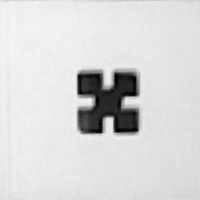
\includegraphics[scale=0.3]{images/tile3.jpg}
\hspace{0.1cm}
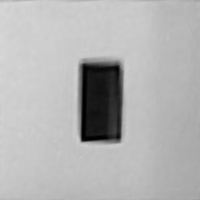
\includegraphics[scale=0.3]{images/tile4.jpg}
\caption{The five cropped individual images of the tiles.}
\label{fig:individ}
\end{minipage}
\end{figure}

\subsection{Comparison}
The last phase of the project is to find the object that will fit into the cavity tile that is extracted from the input image. This last phase is approached by comparing the extracted image with all the possible orientations of the tile stored in the database.  
\subsubsection*{creating Database}
\begin{itemize}
\item There are eleven tiles used in the competition. 
\item  In the eleven tile 
\begin{itemize}
\item five tiles have only one possible orientation


\begin{figure}[h!]
\begin{minipage}{\textwidth}
\centering
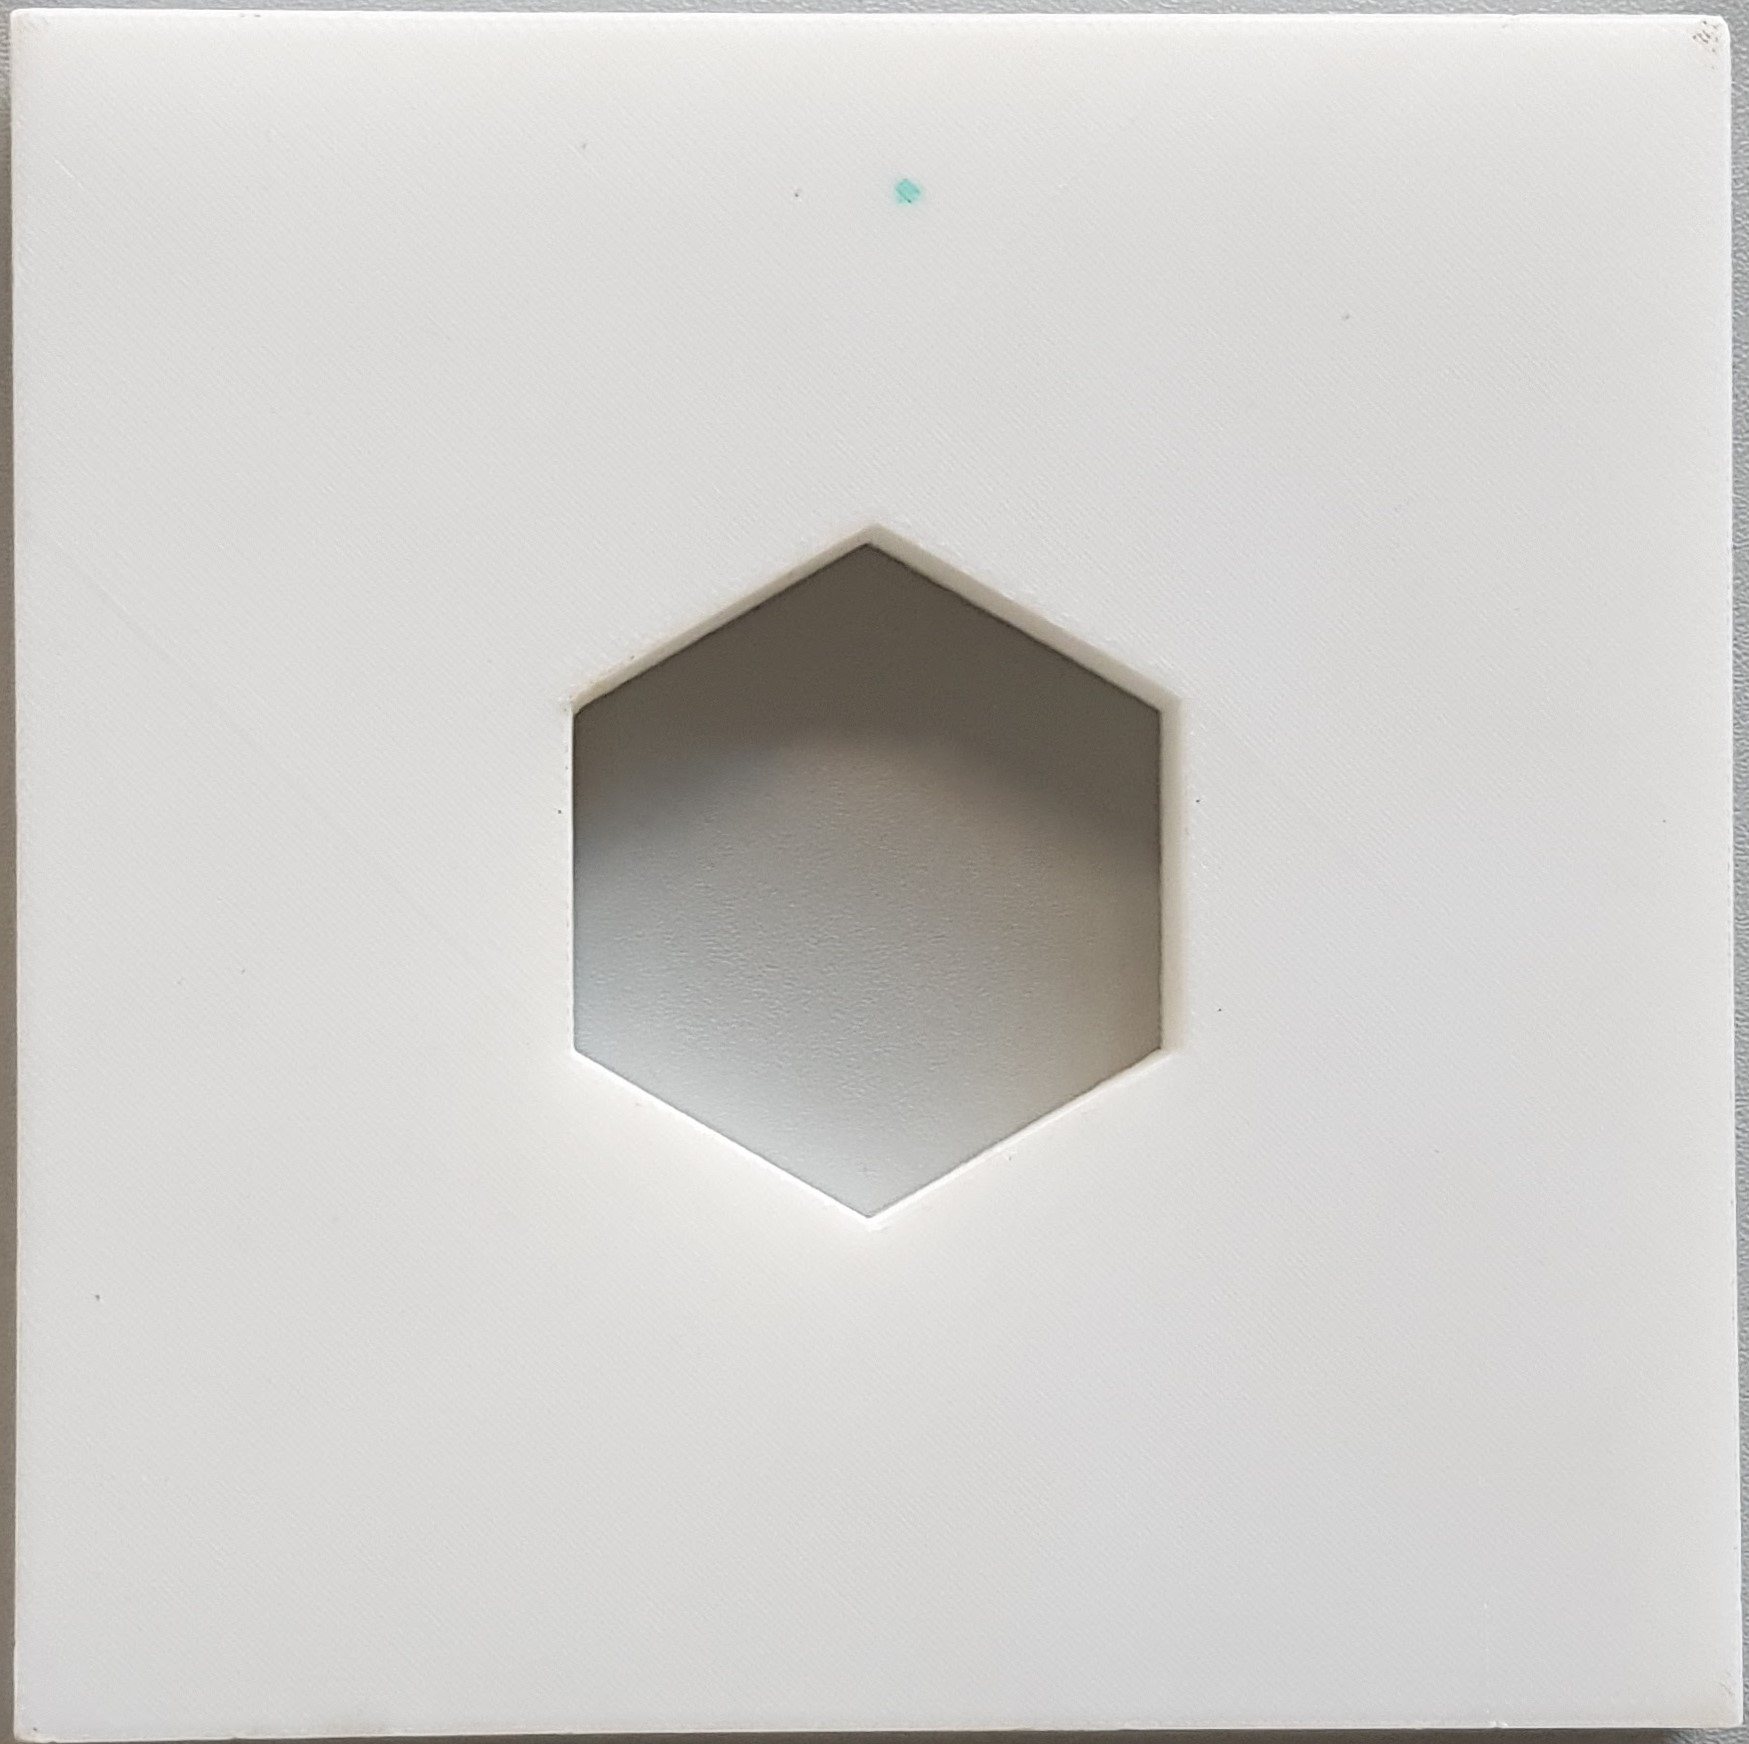
\includegraphics[width = 2.5 cm, height = 2.5 cm]{images/tile01.jpg}
\hspace{0.1cm}
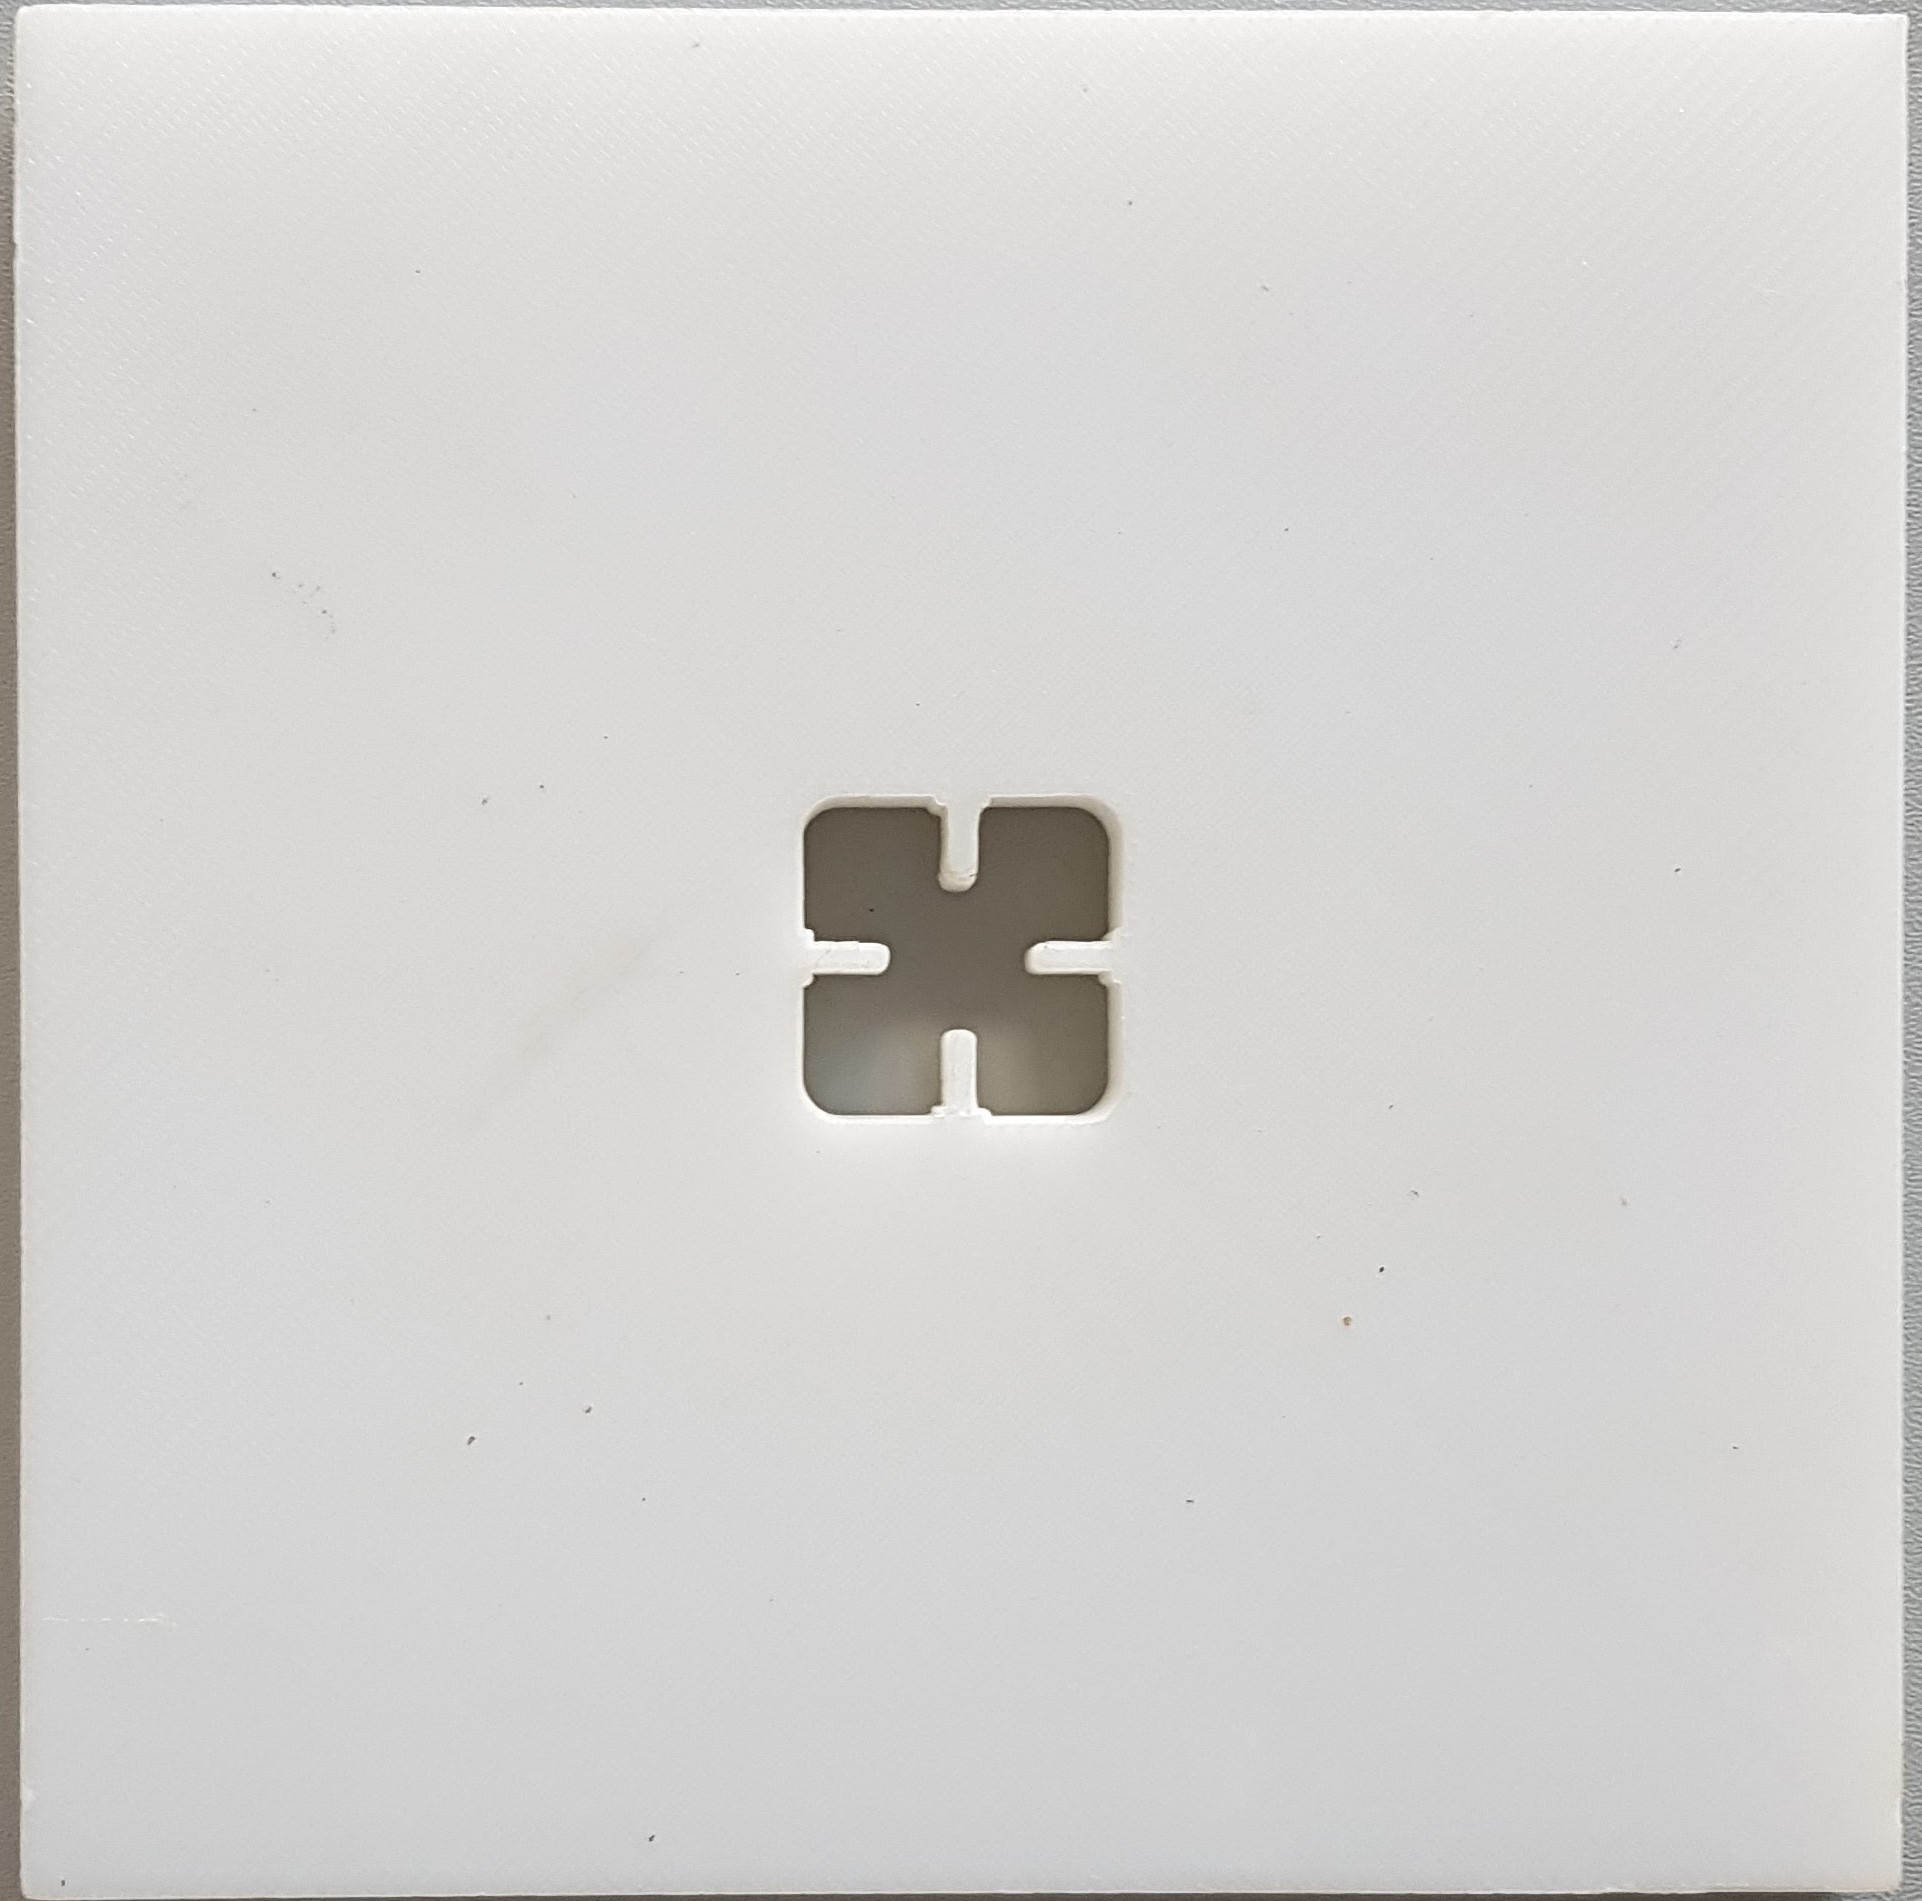
\includegraphics[width = 2.5 cm, height = 2.5 cm]{images/tile02.jpg}
\hspace{0.1cm}
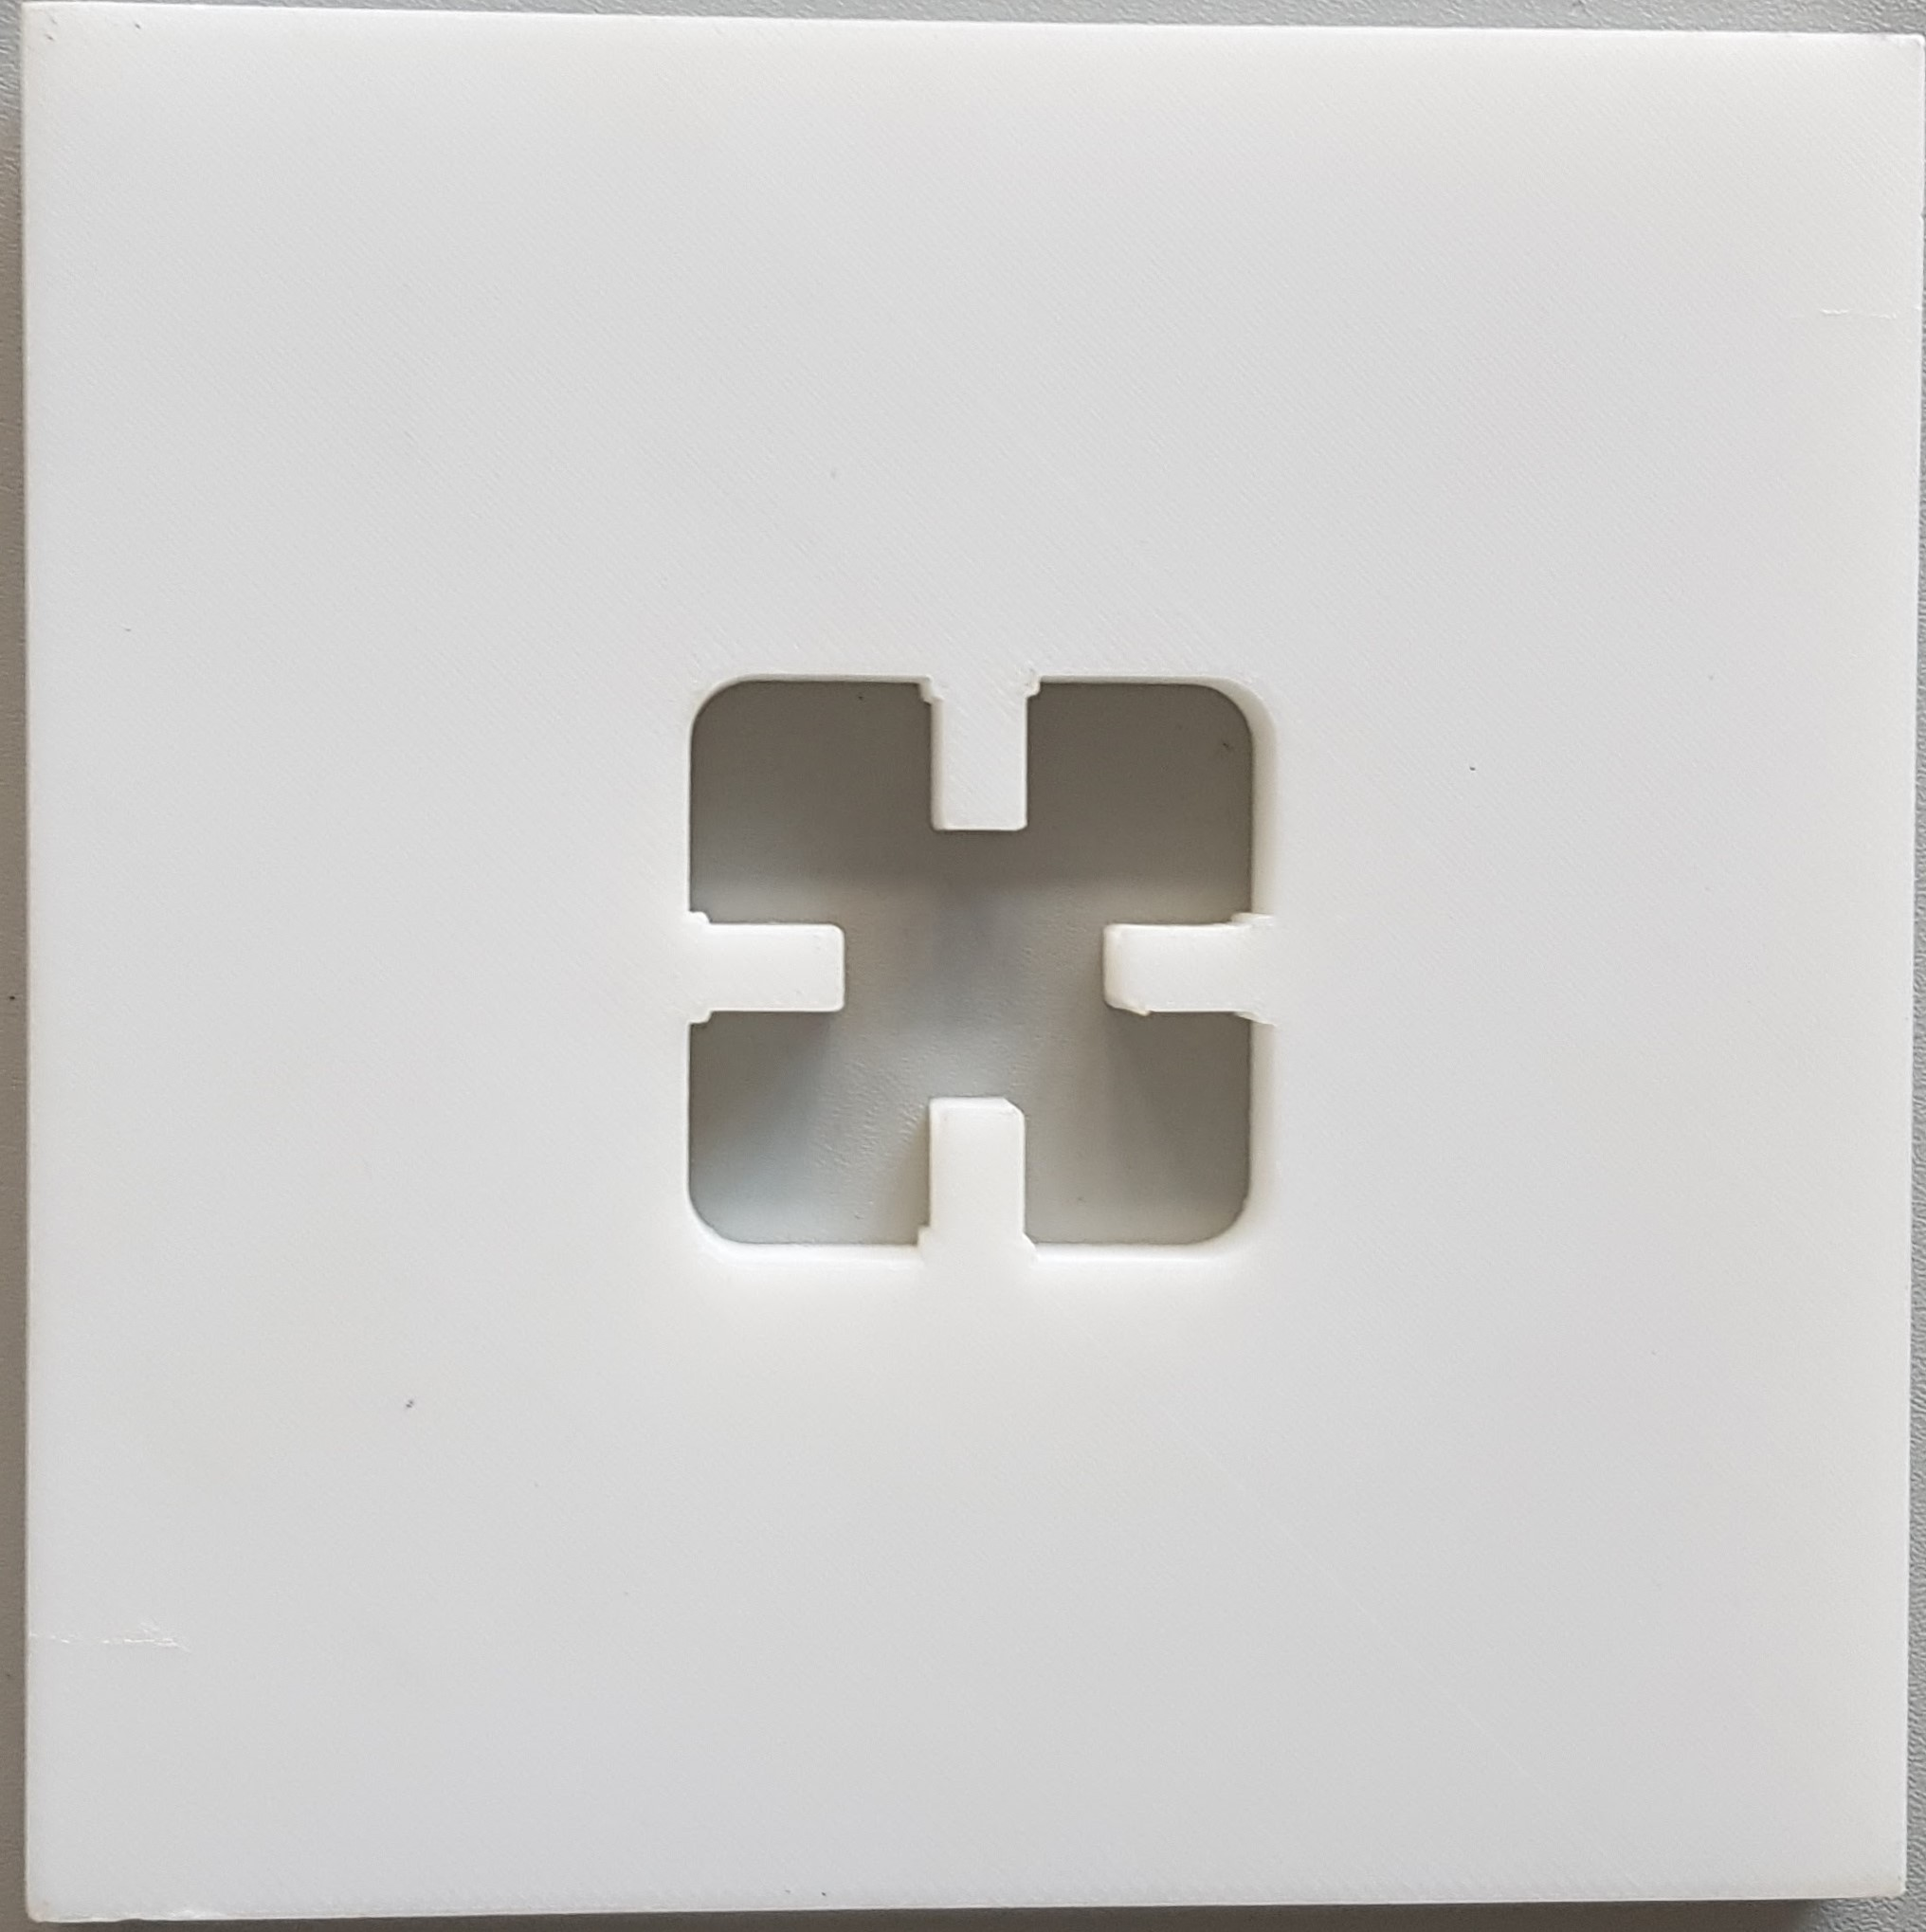
\includegraphics[width = 2.5 cm, height = 2.5 cm]{images/tile03.jpg}
\hspace{0.1cm}
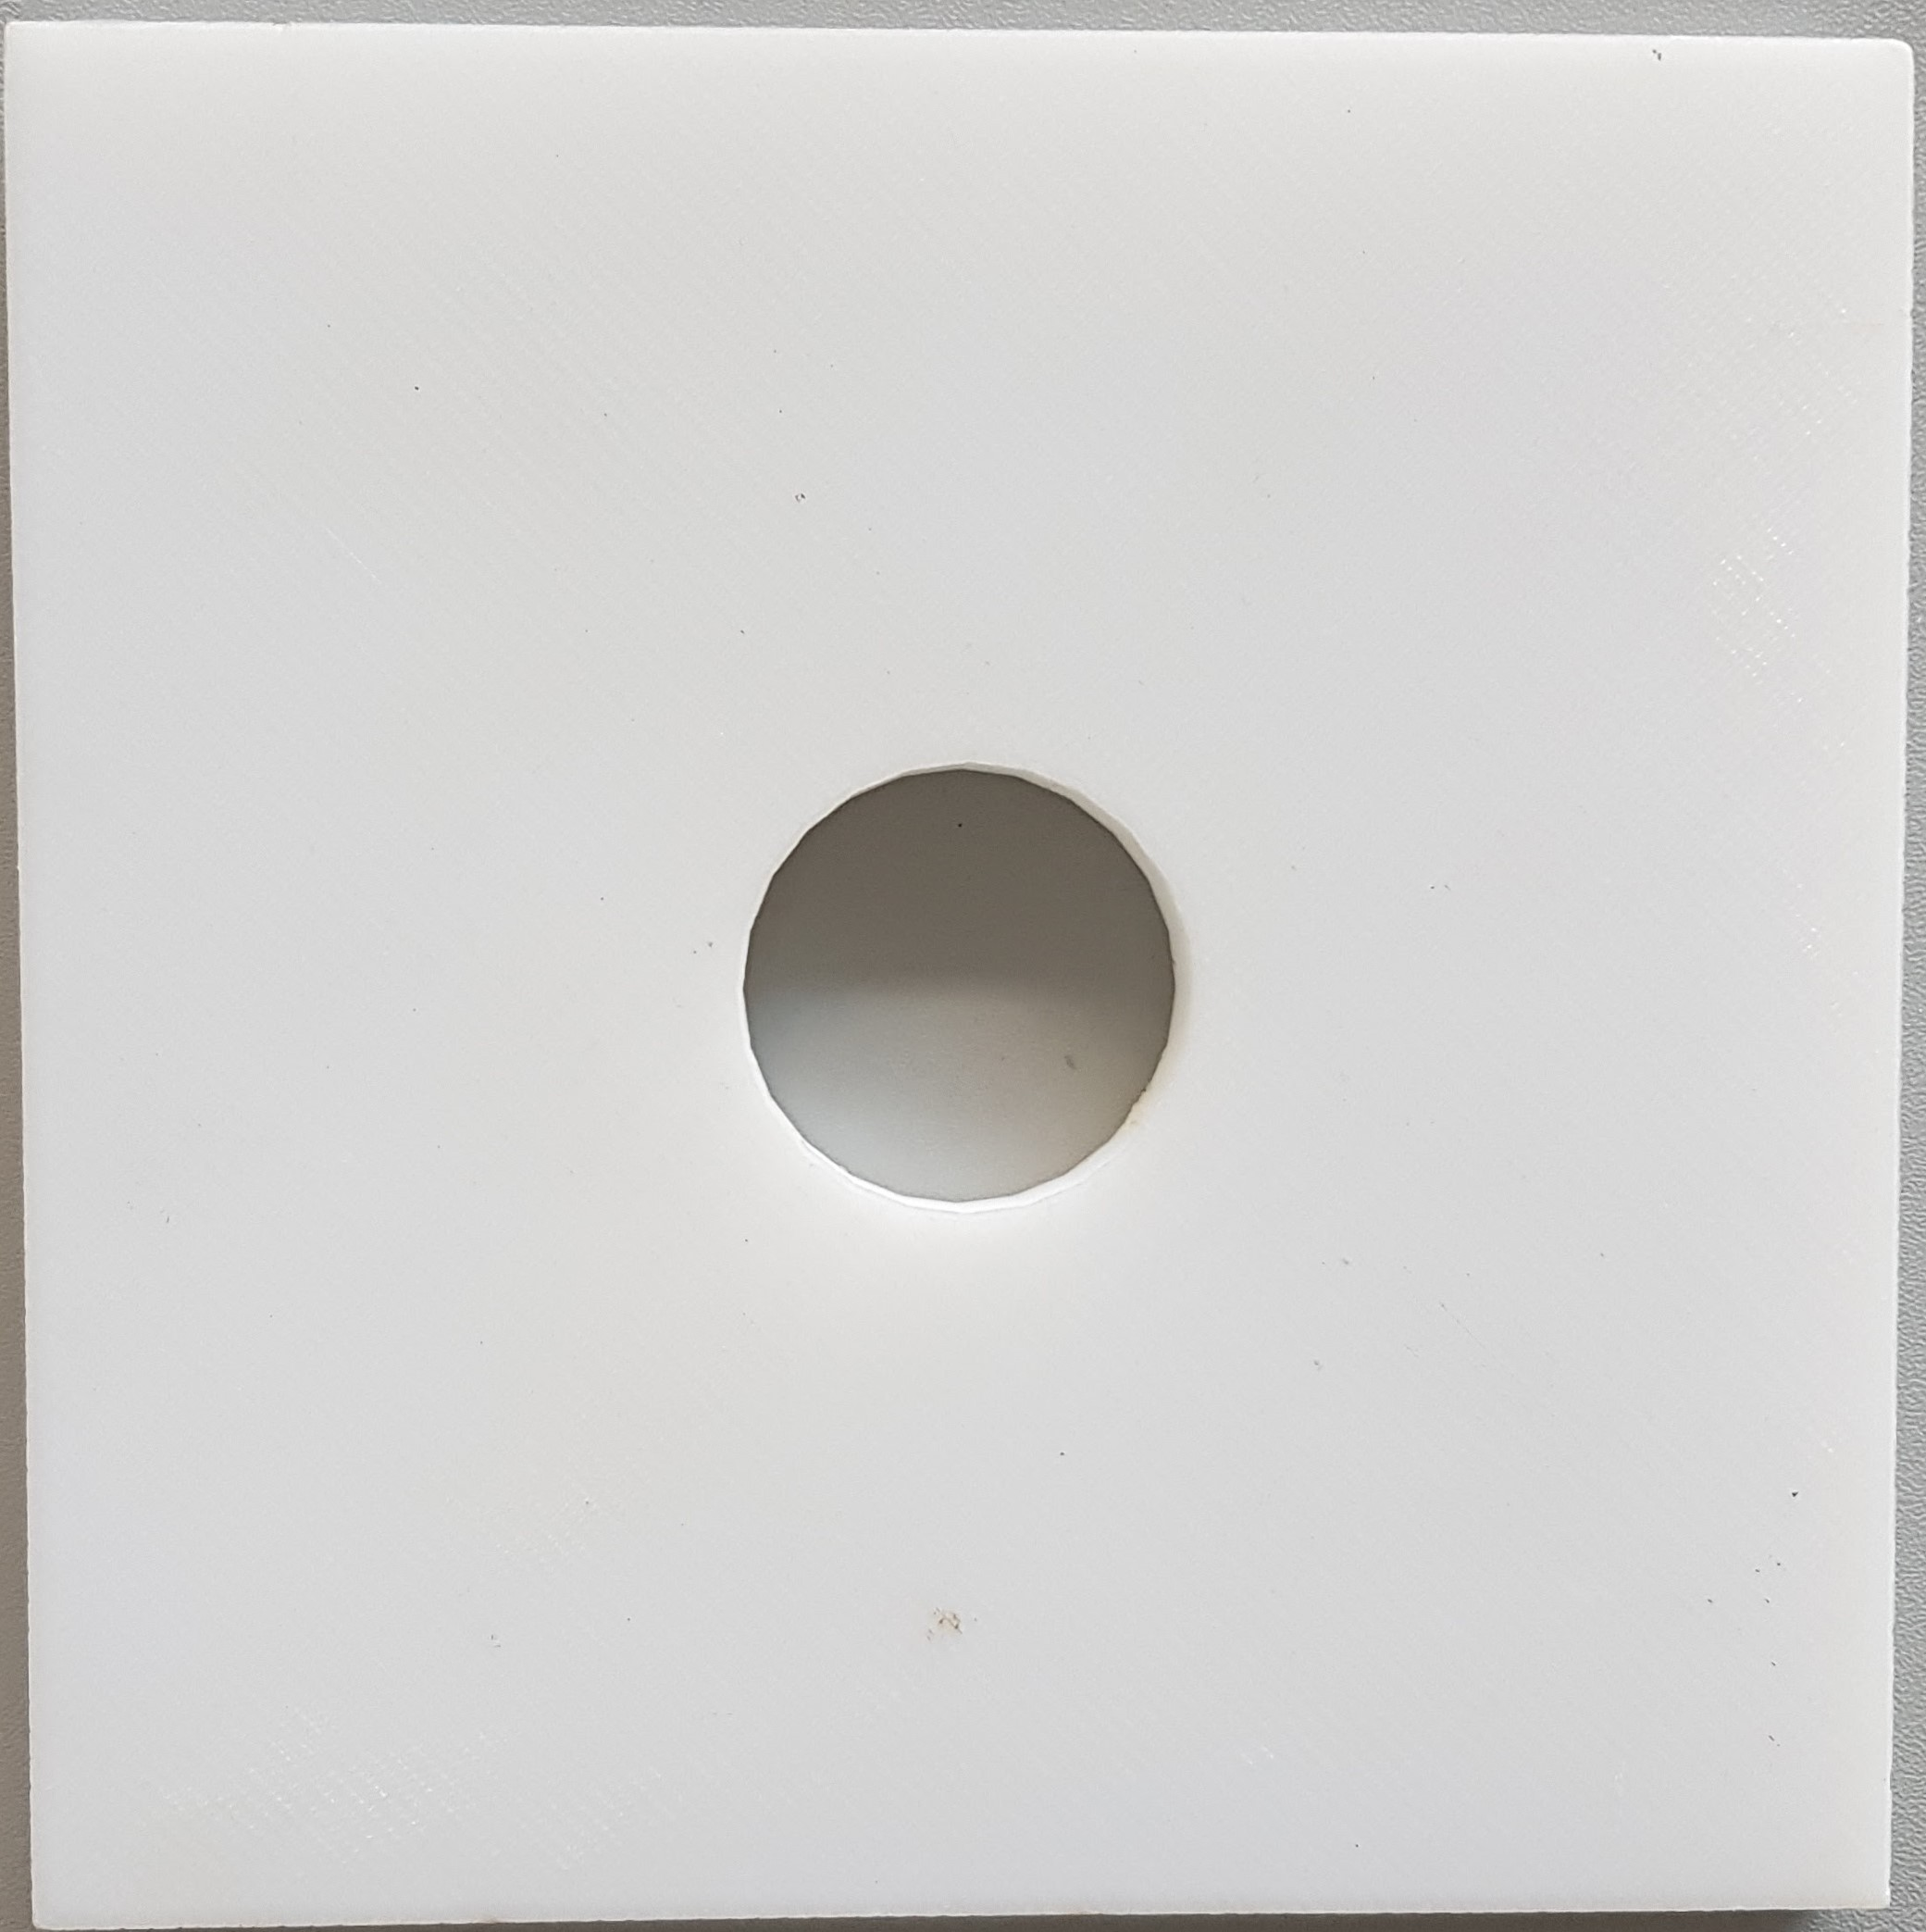
\includegraphics[width = 2.5 cm, height = 2.5 cm]{images/tile04.jpg}
\hspace{0.1cm}
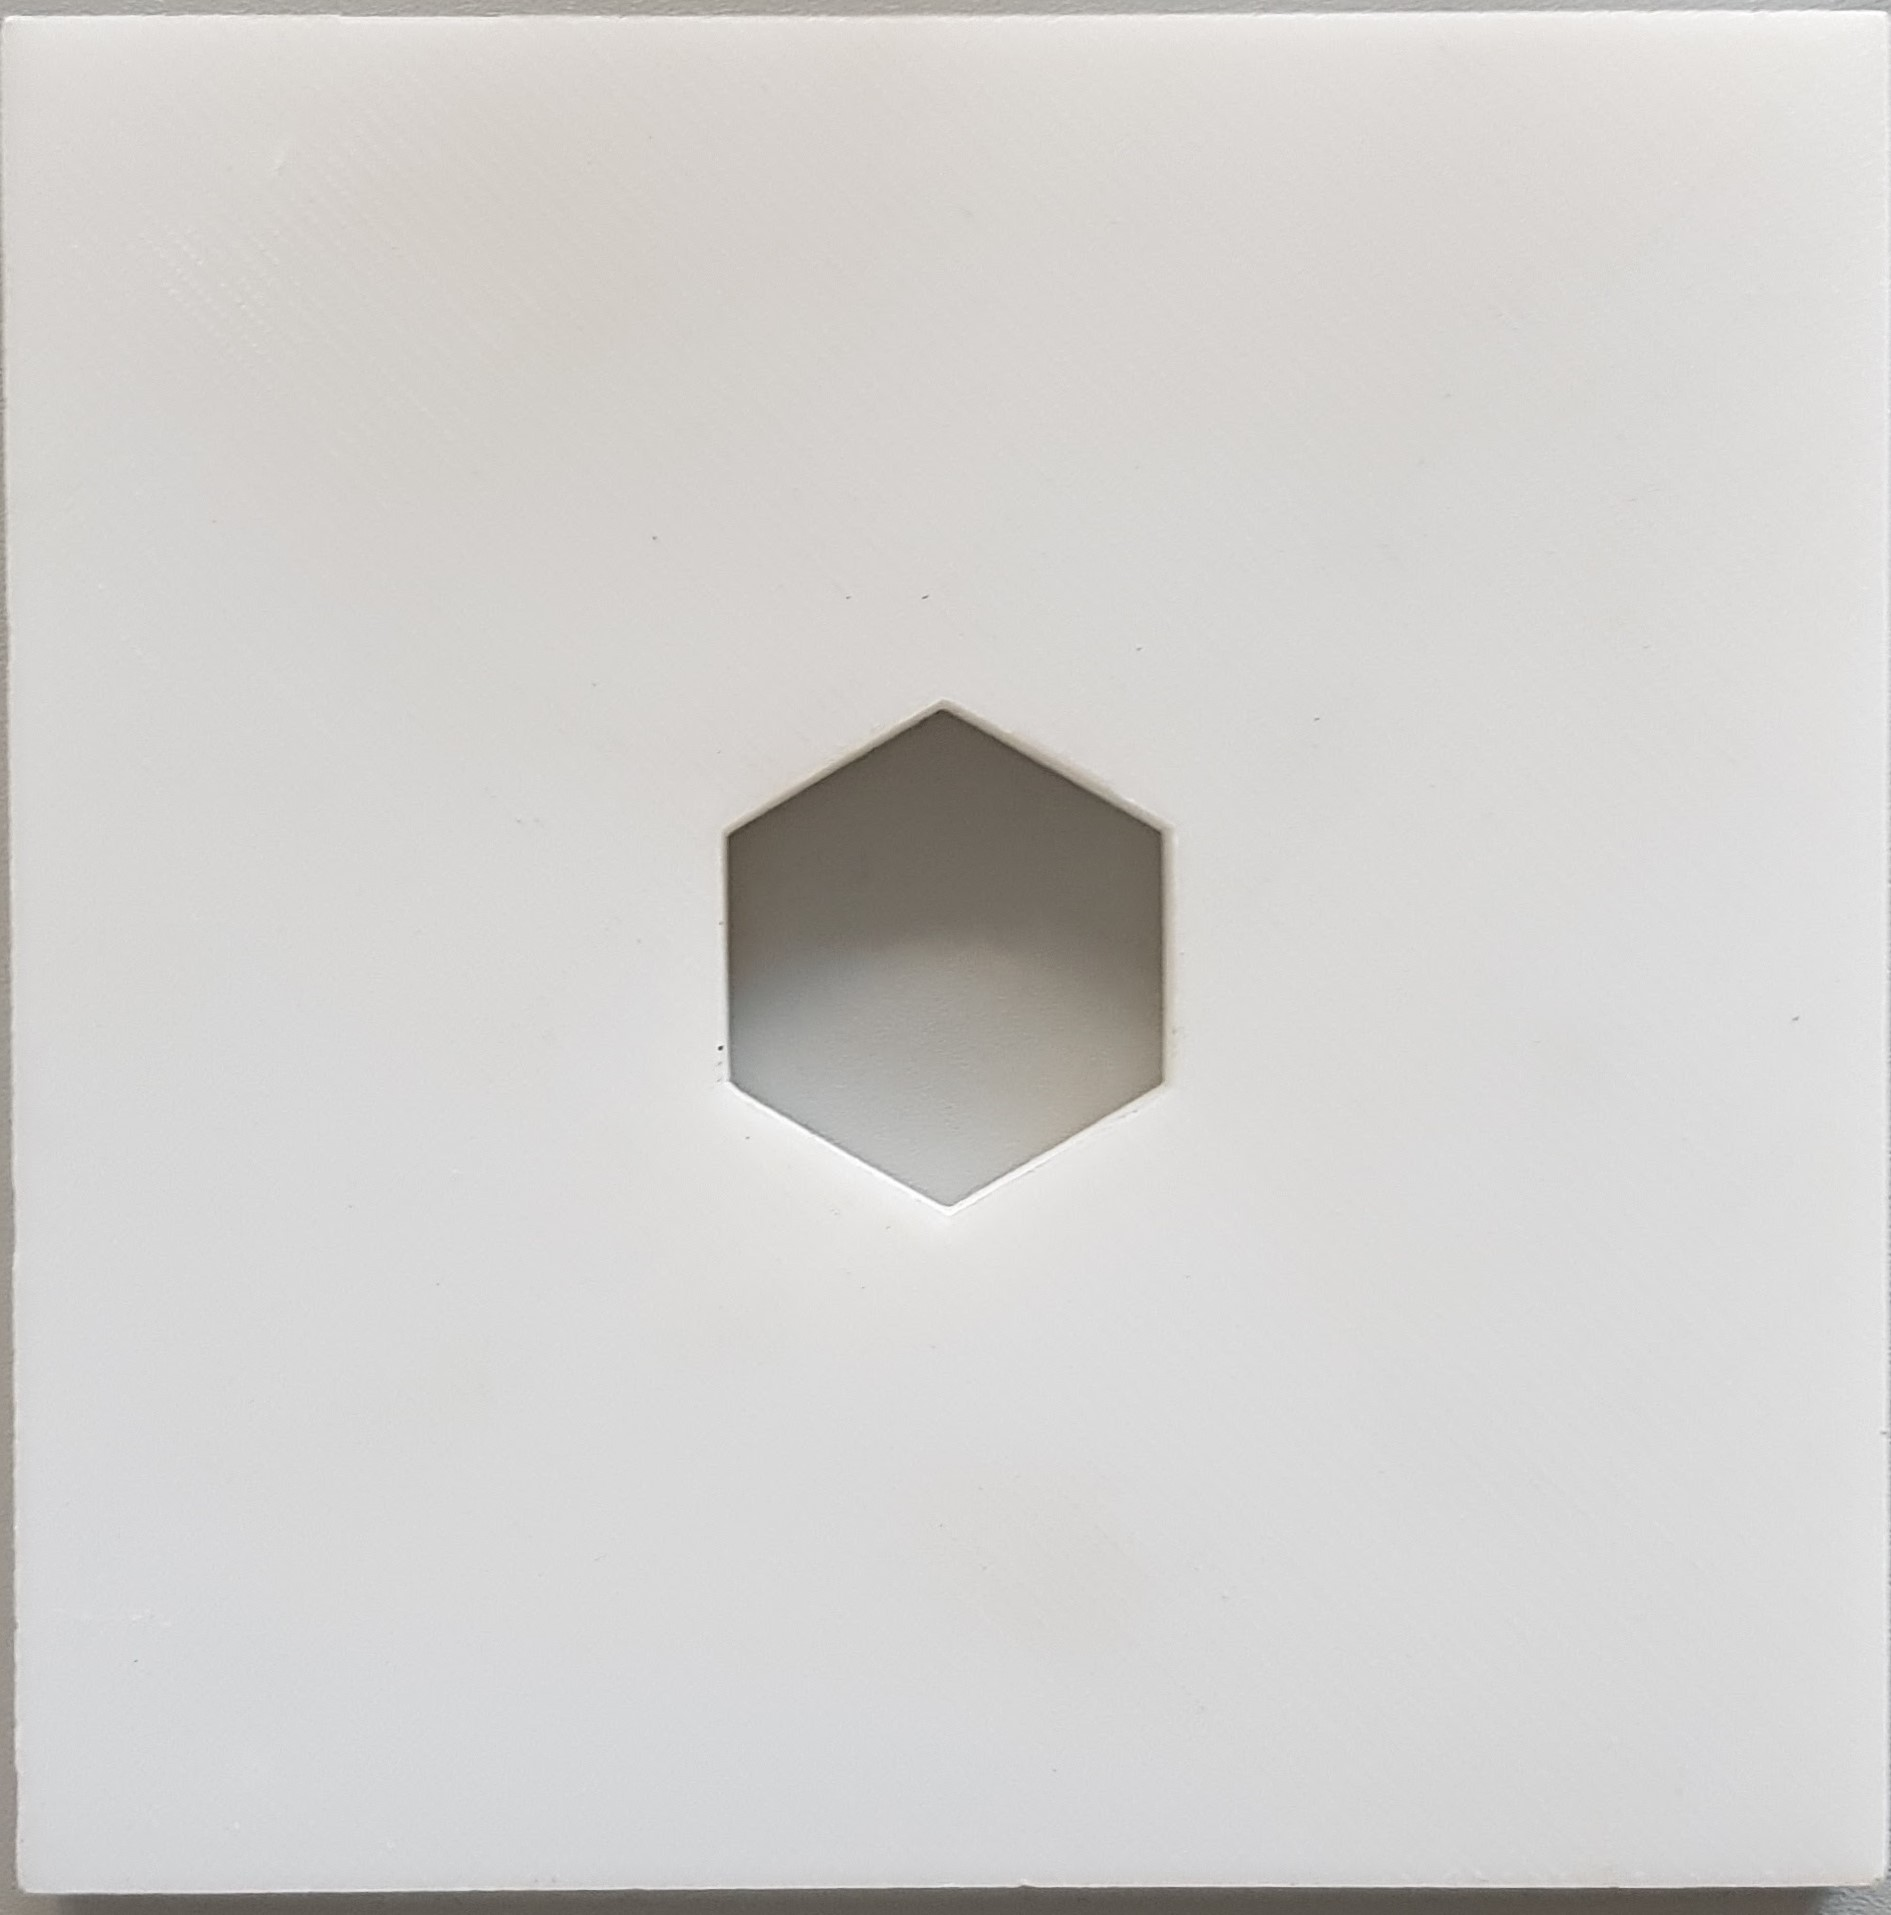
\includegraphics[width = 2.5 cm, height = 2.5 cm]{images/tile05.jpg}
\caption{Tiles with one possible orientation}
\label{fig:onepossibility}
\end{minipage}
\end{figure}


\item Cavity tiles have two possible orientation

\begin{figure}[h!]
\begin{minipage}{\textwidth}
\centering
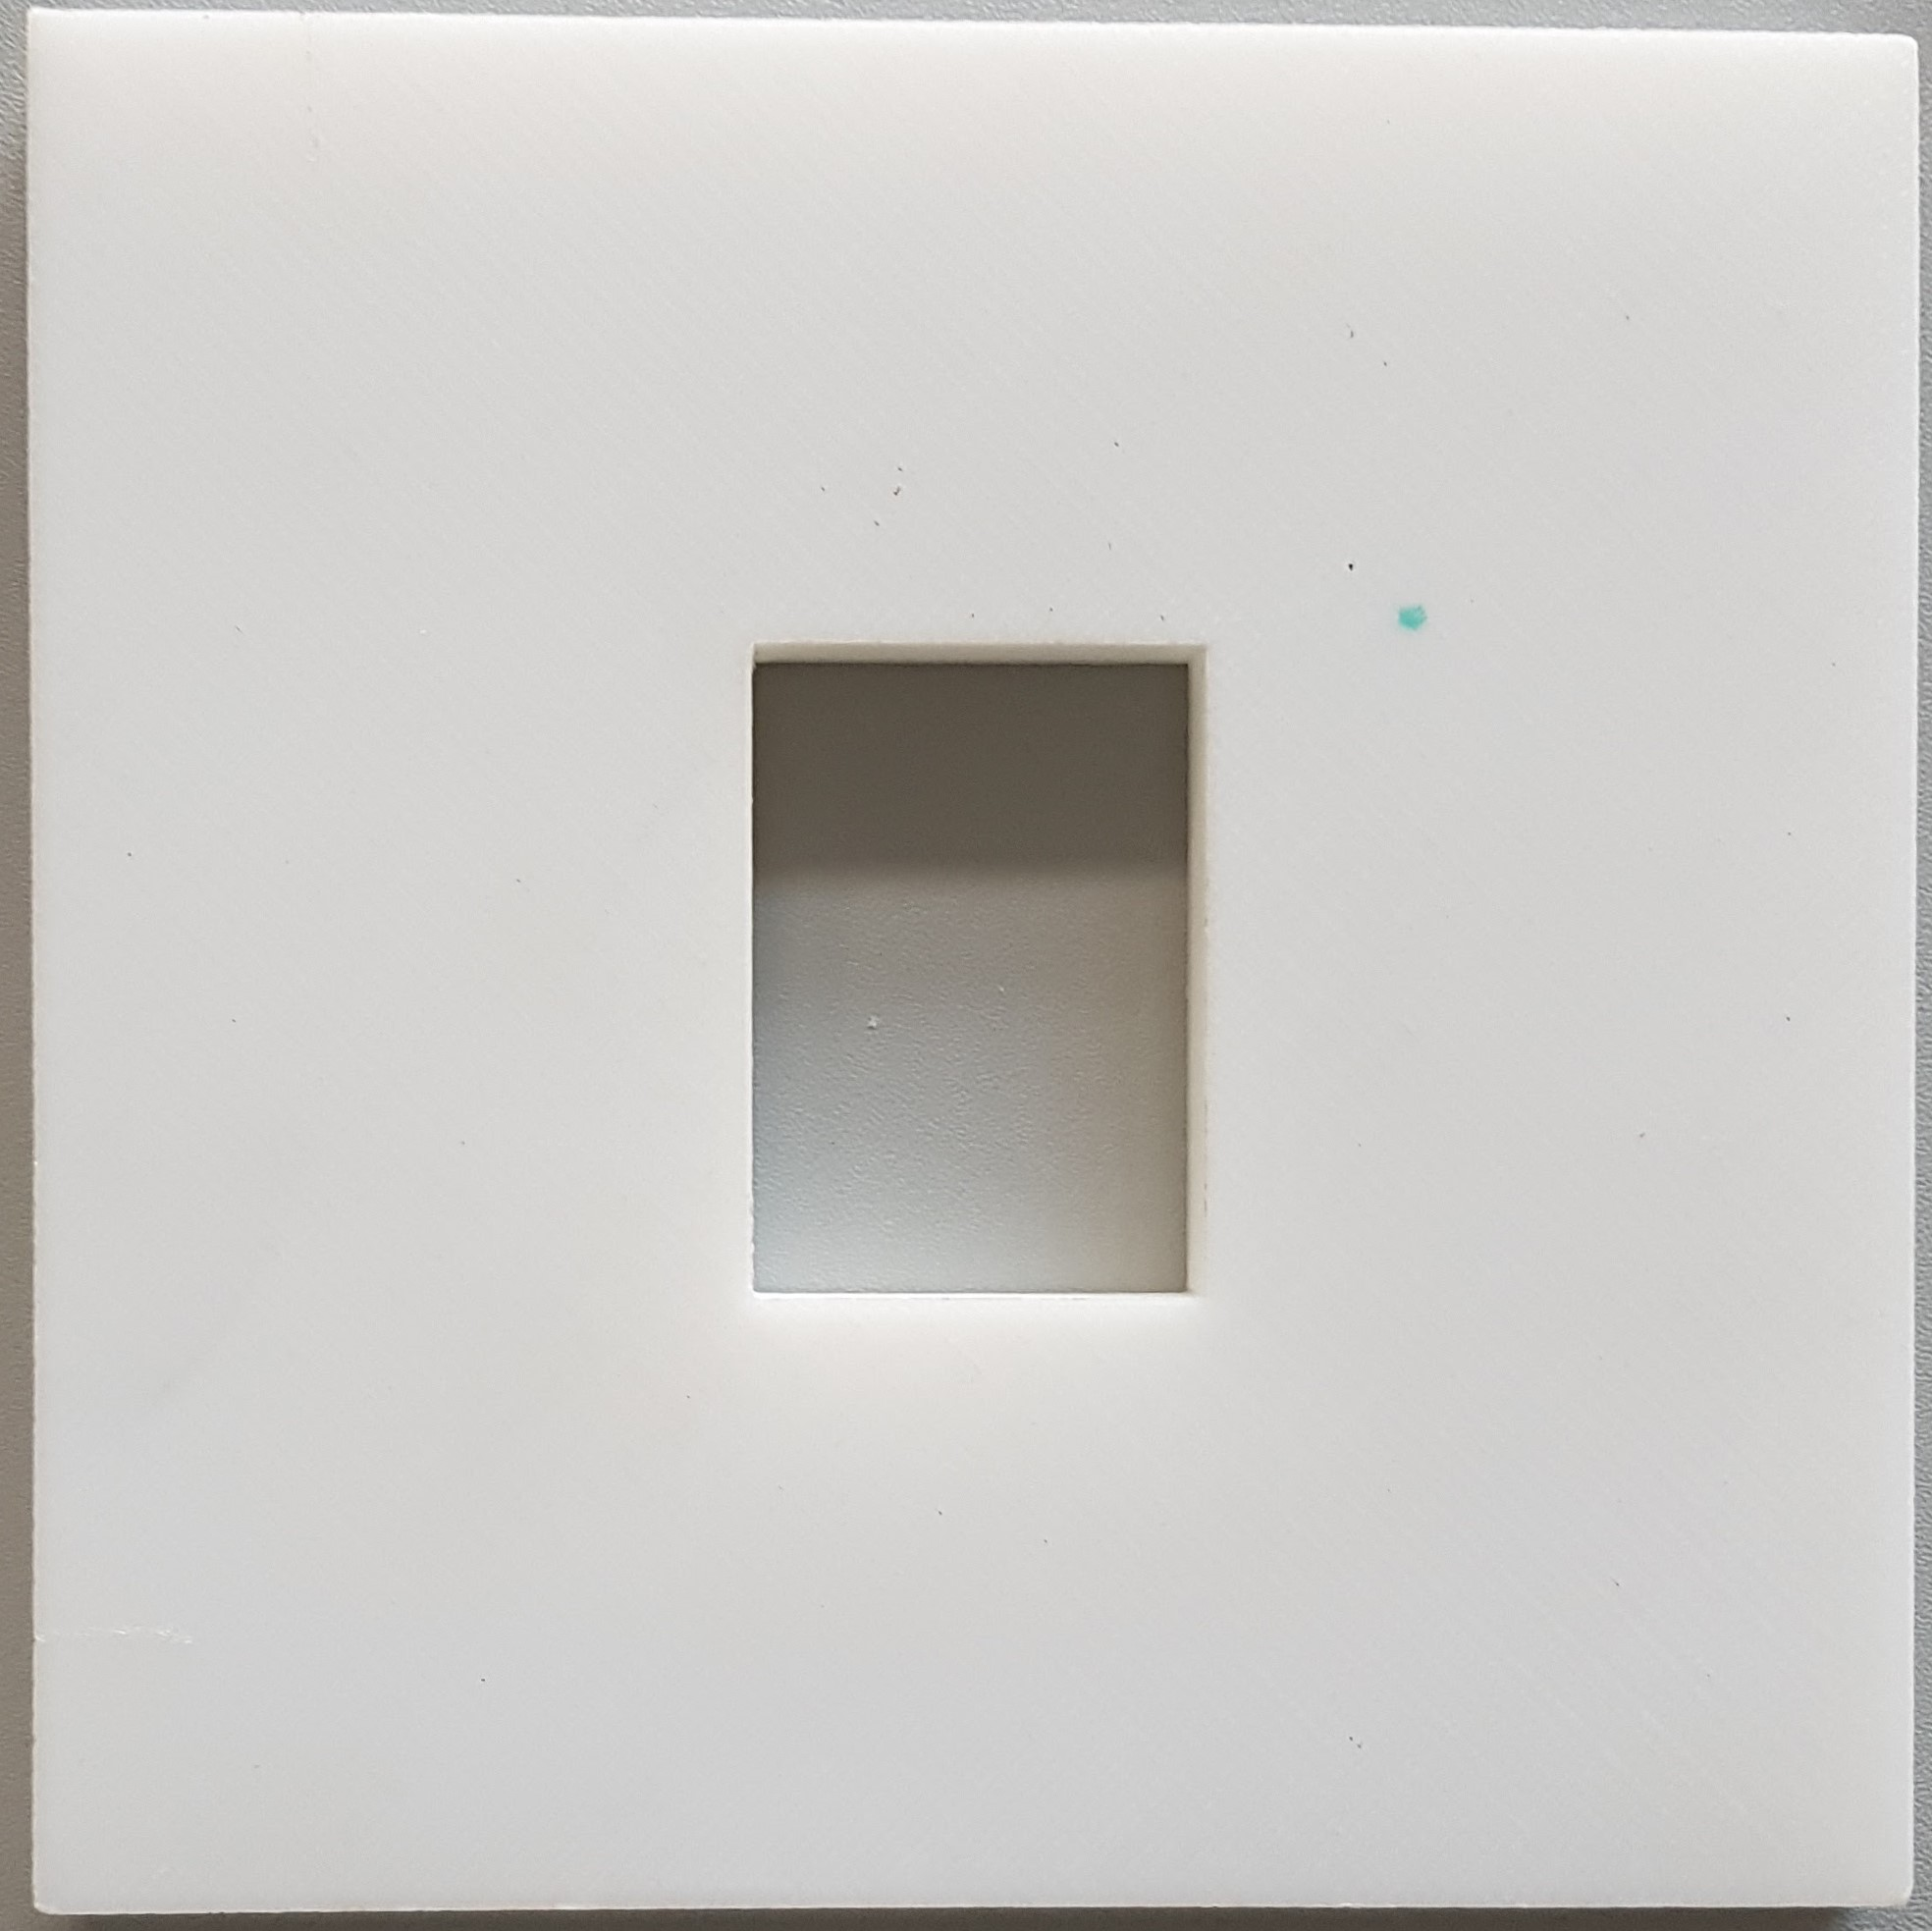
\includegraphics[width = 2.5 cm, height = 2.5 cm]{images/tile06.jpg}
\hspace{0.1cm}
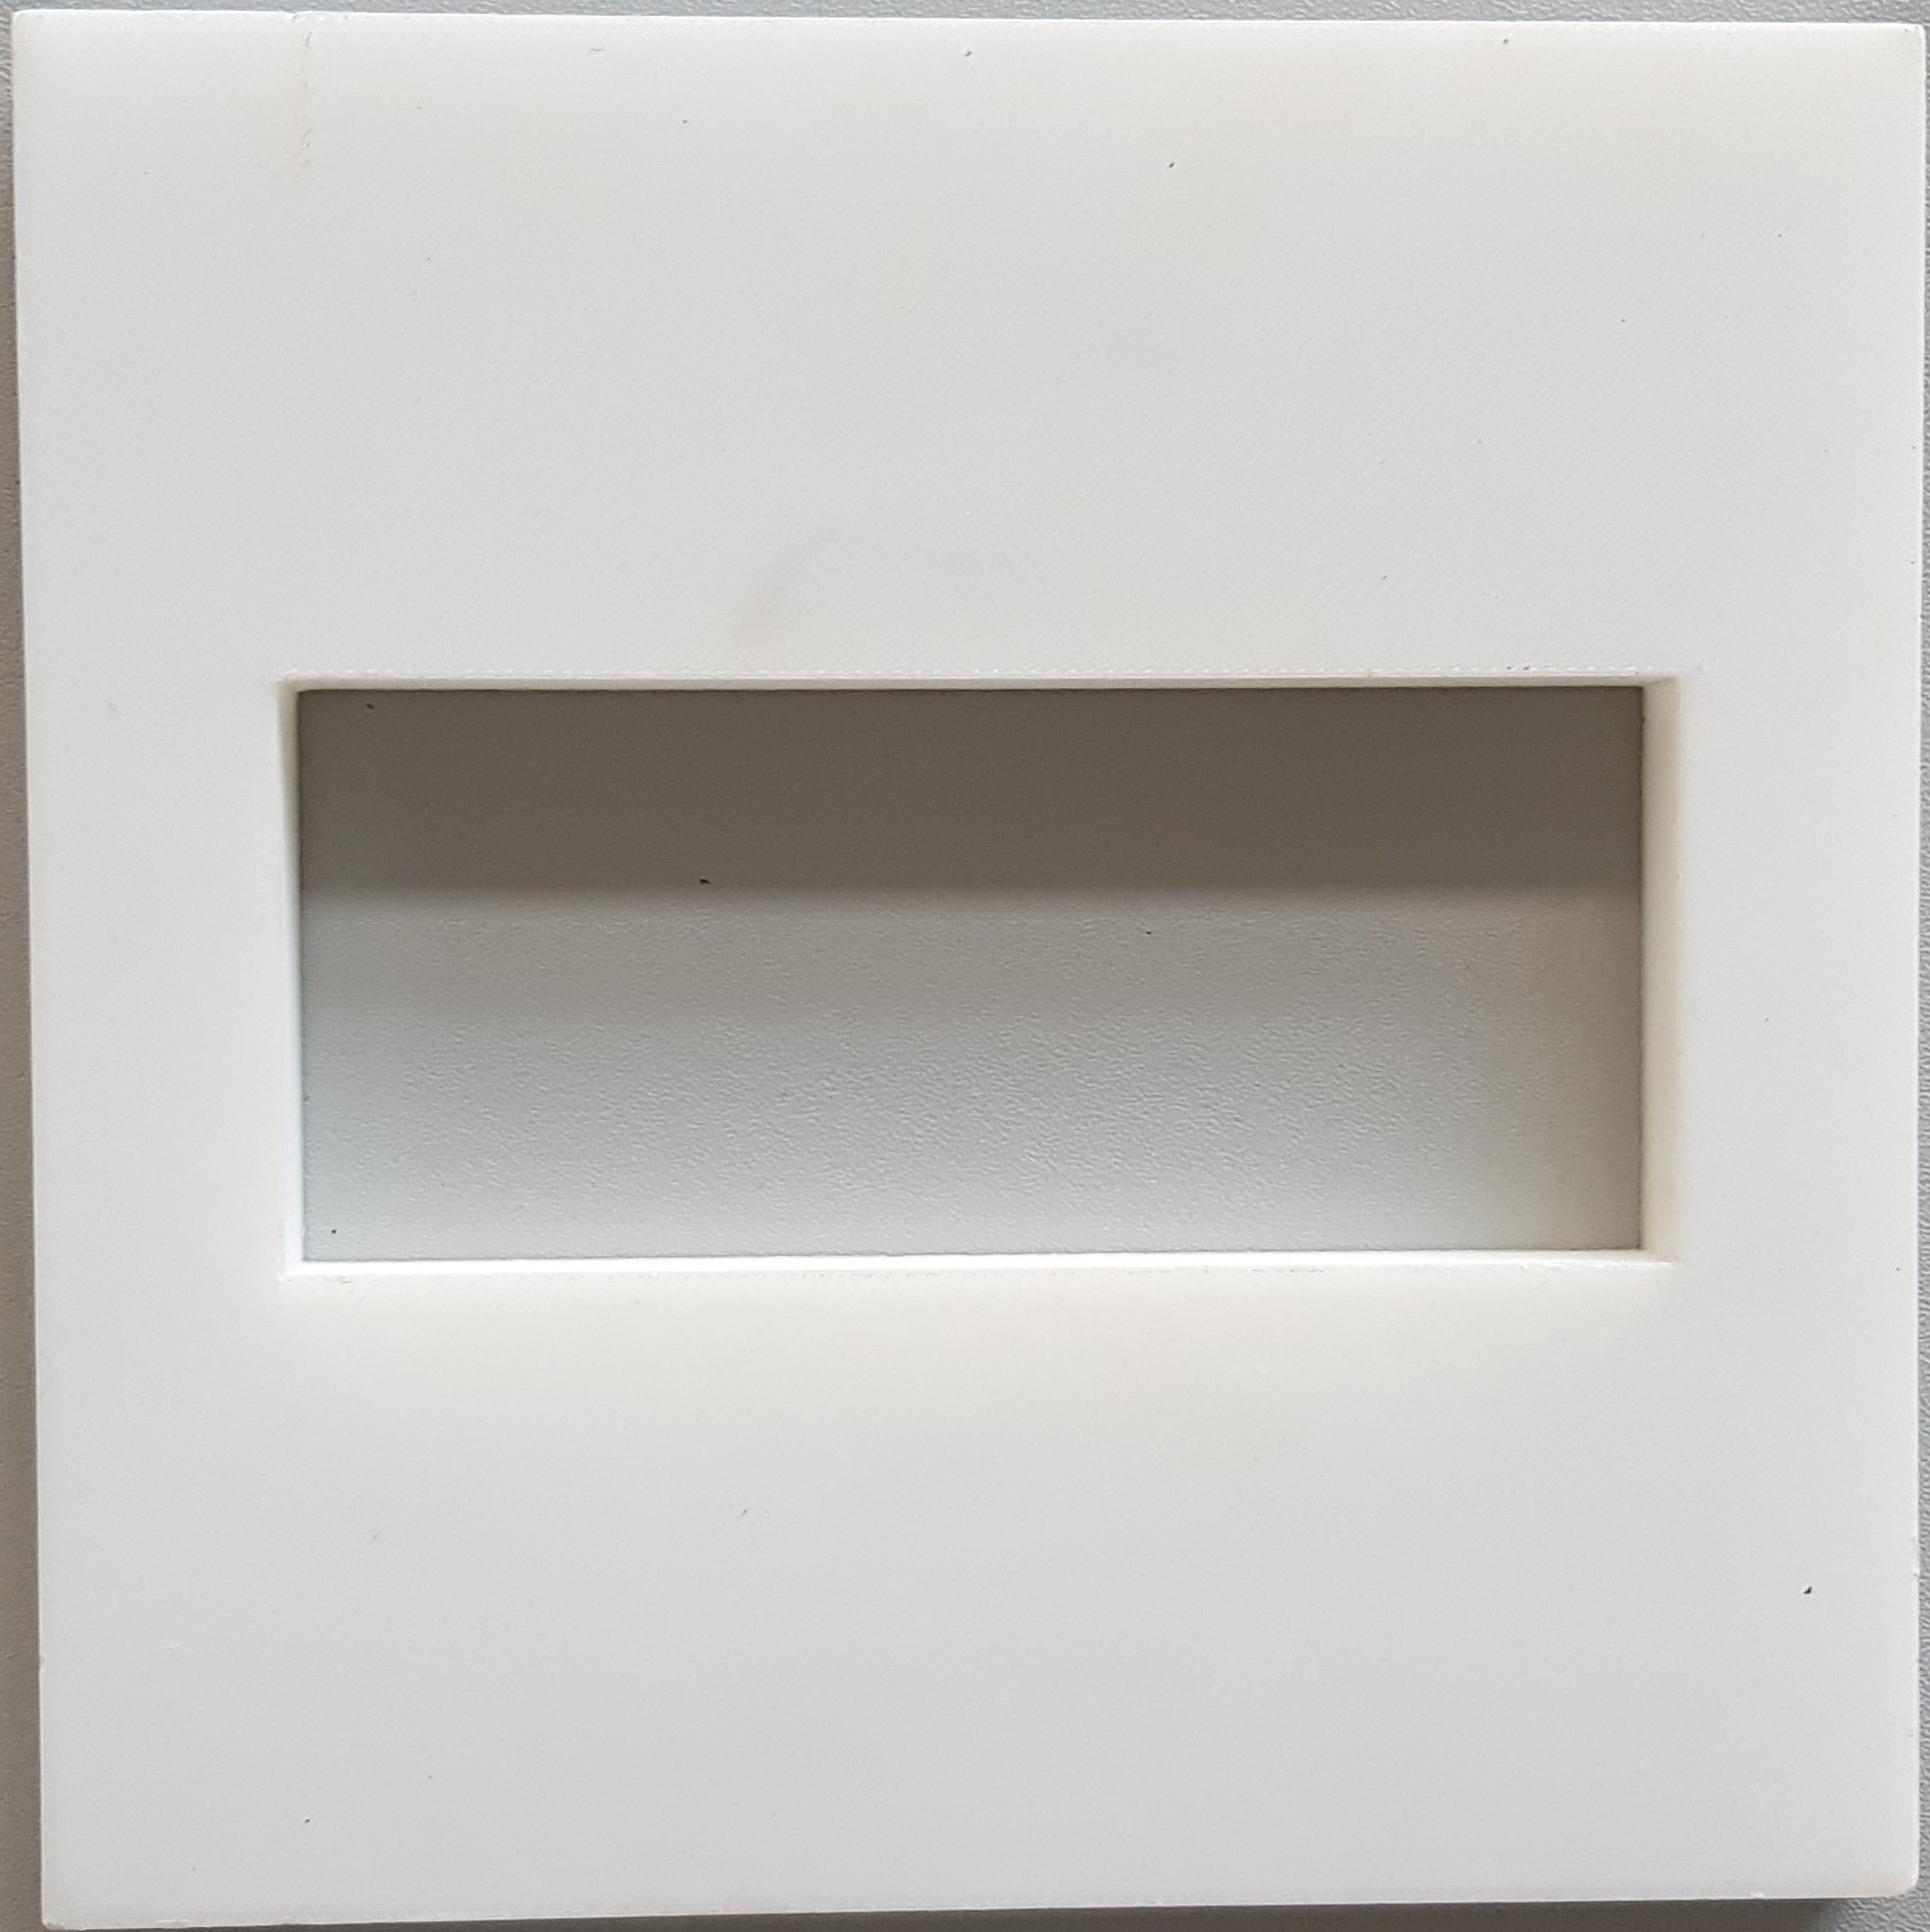
\includegraphics[width = 2.5 cm, height = 2.5 cm]{images/tile07.jpg}
\hspace{0.1cm}
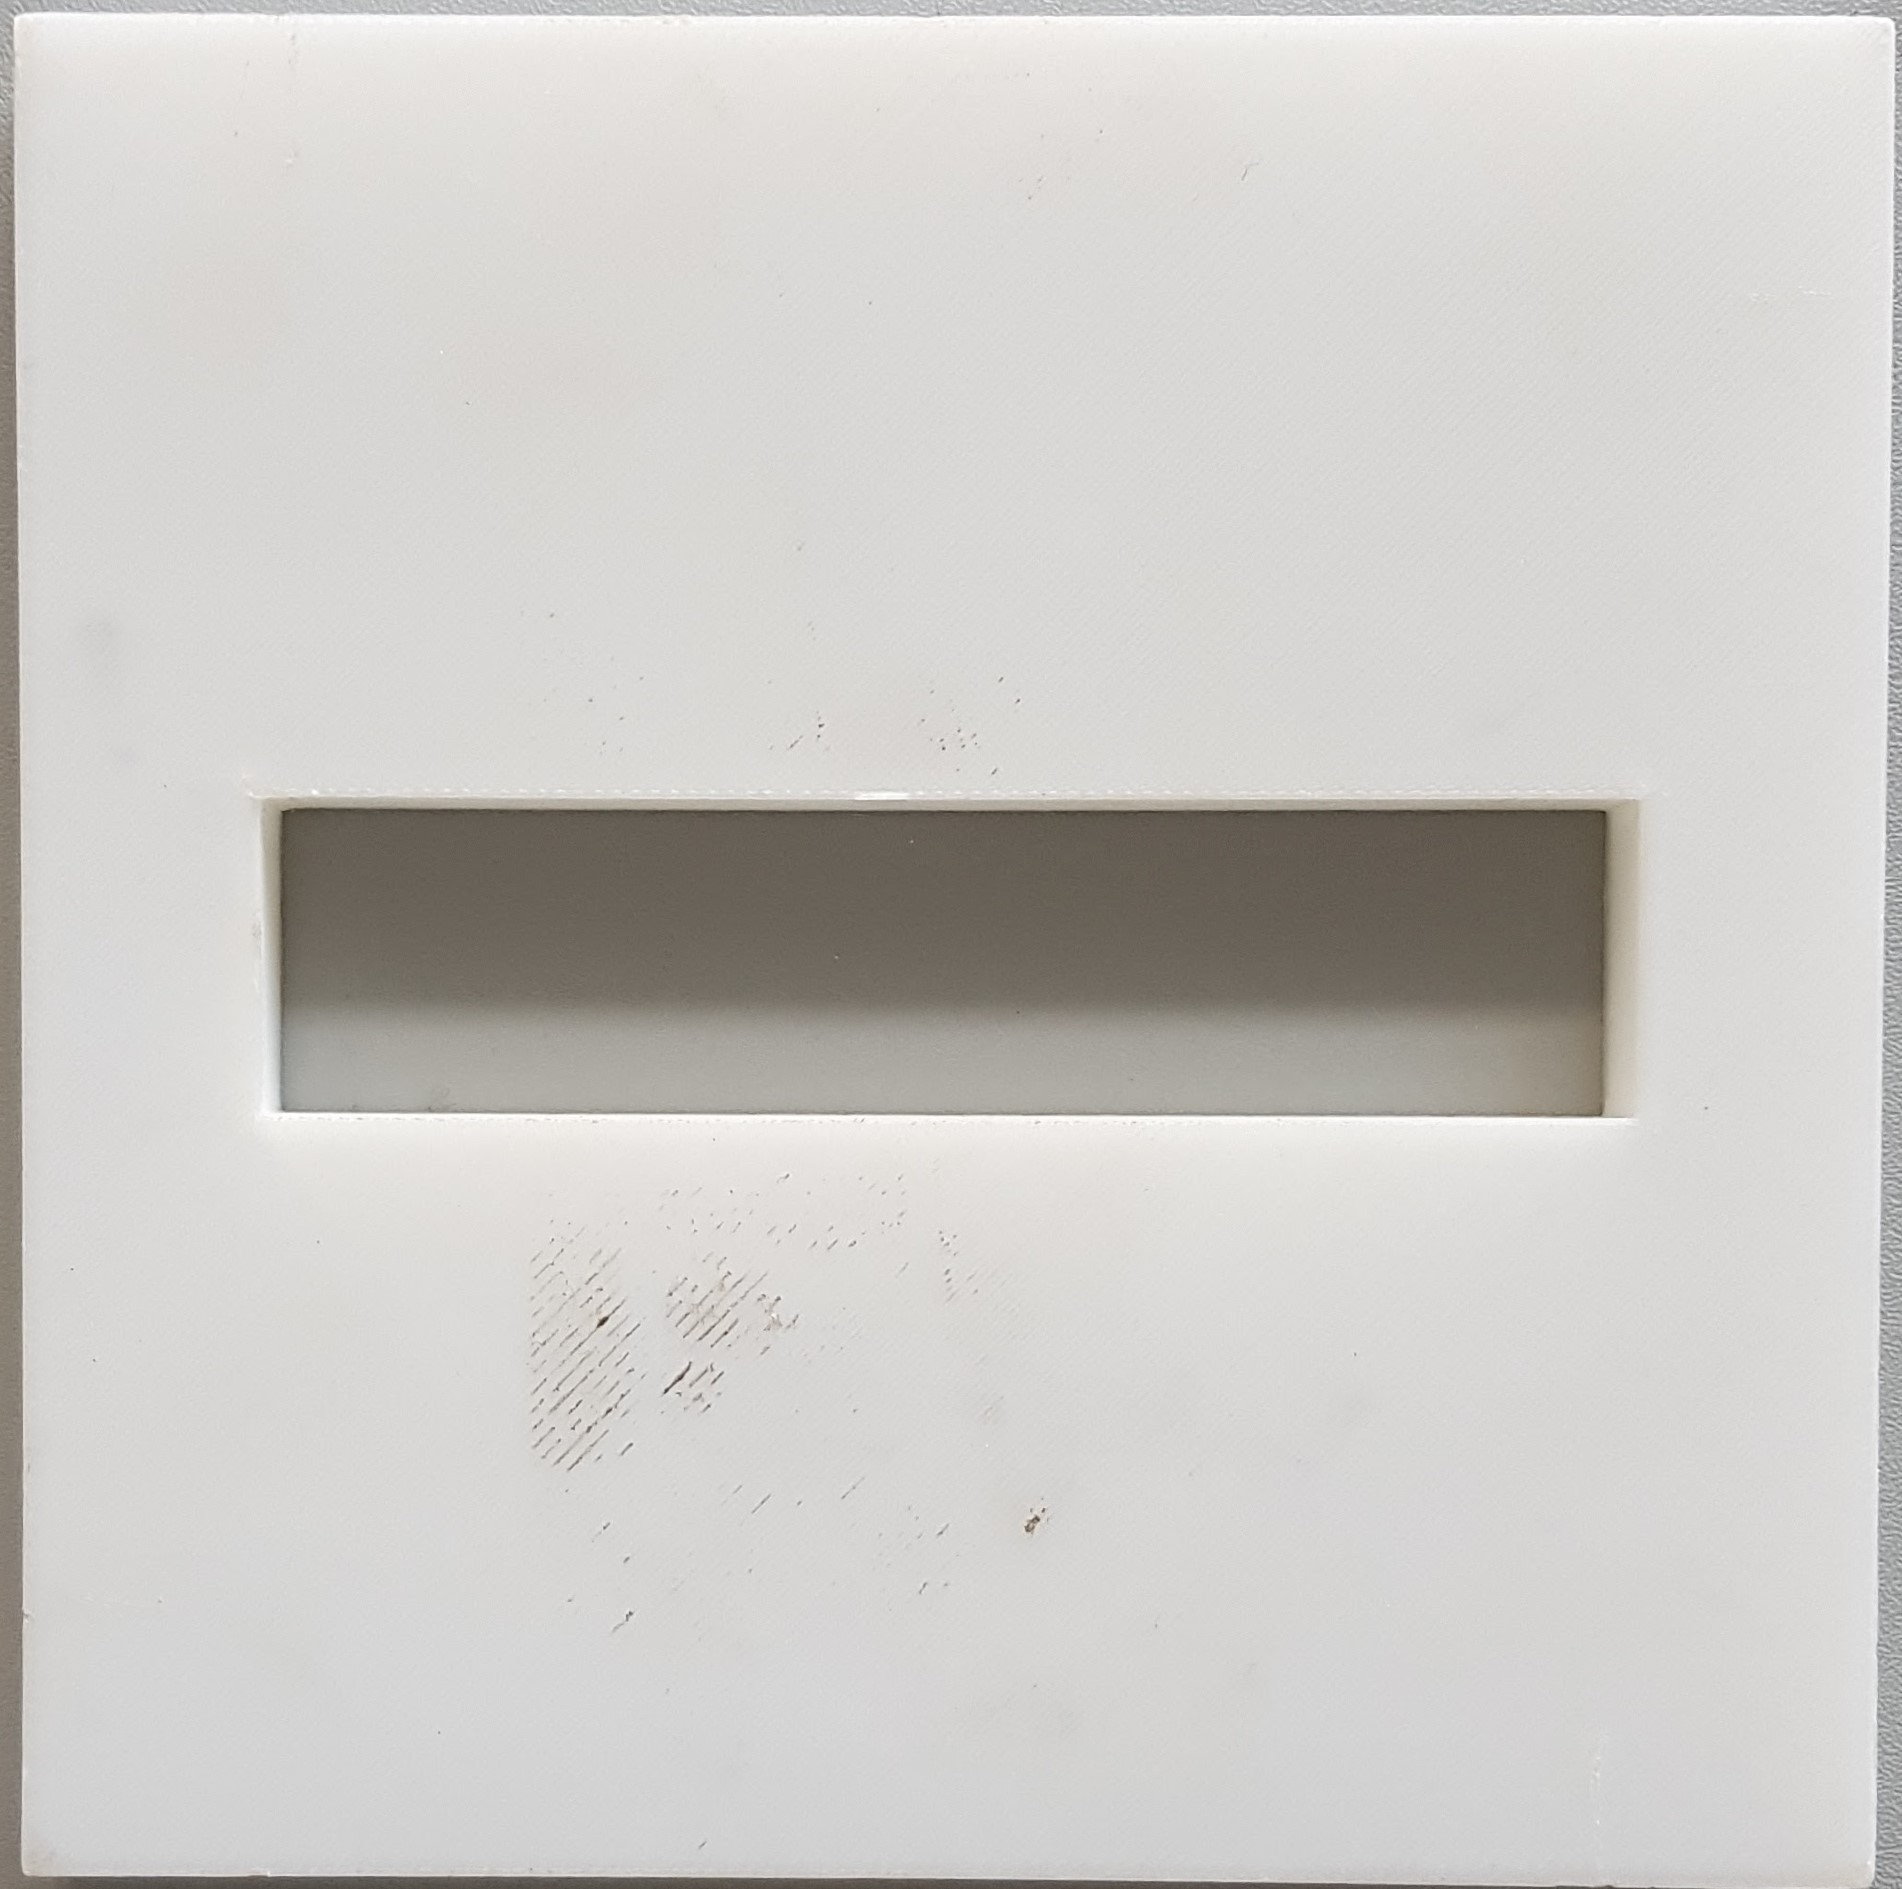
\includegraphics[width = 2.5 cm, height = 2.5 cm]{images/tile08.jpg}
\hspace{0.1cm}
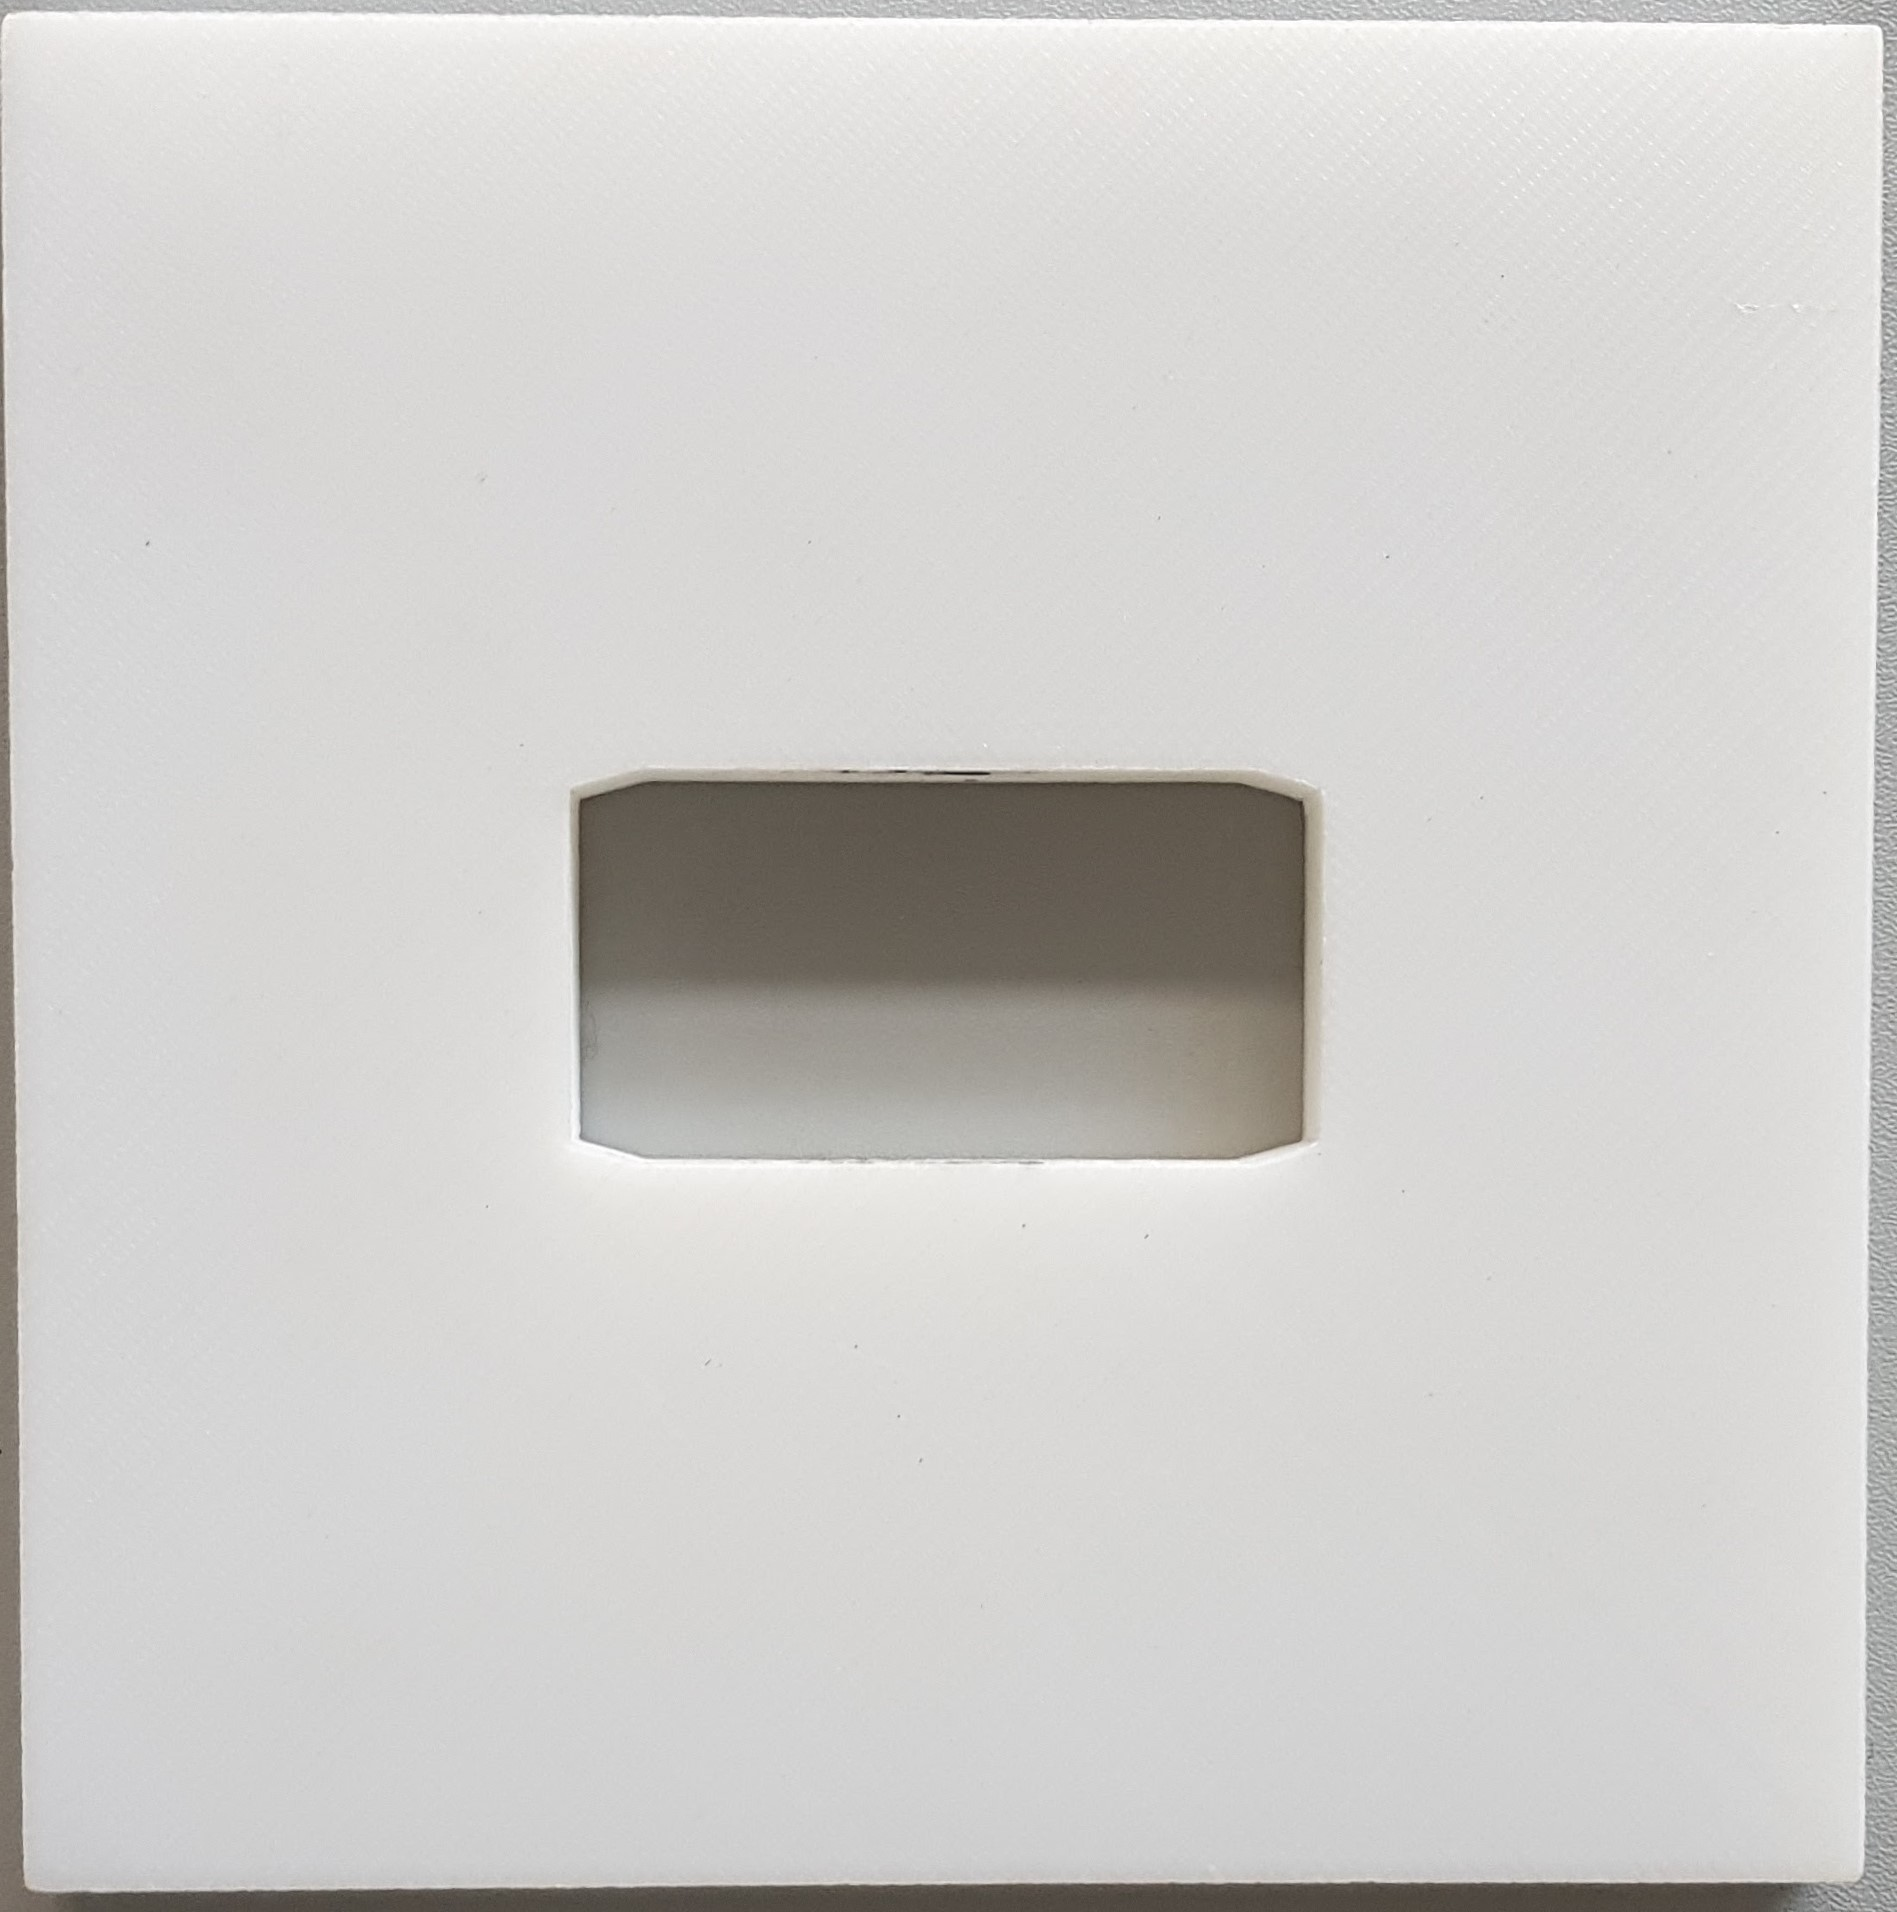
\includegraphics[width = 2.5 cm, height = 2.5 cm]{images/tile09.jpg}
\hspace{0.1cm}
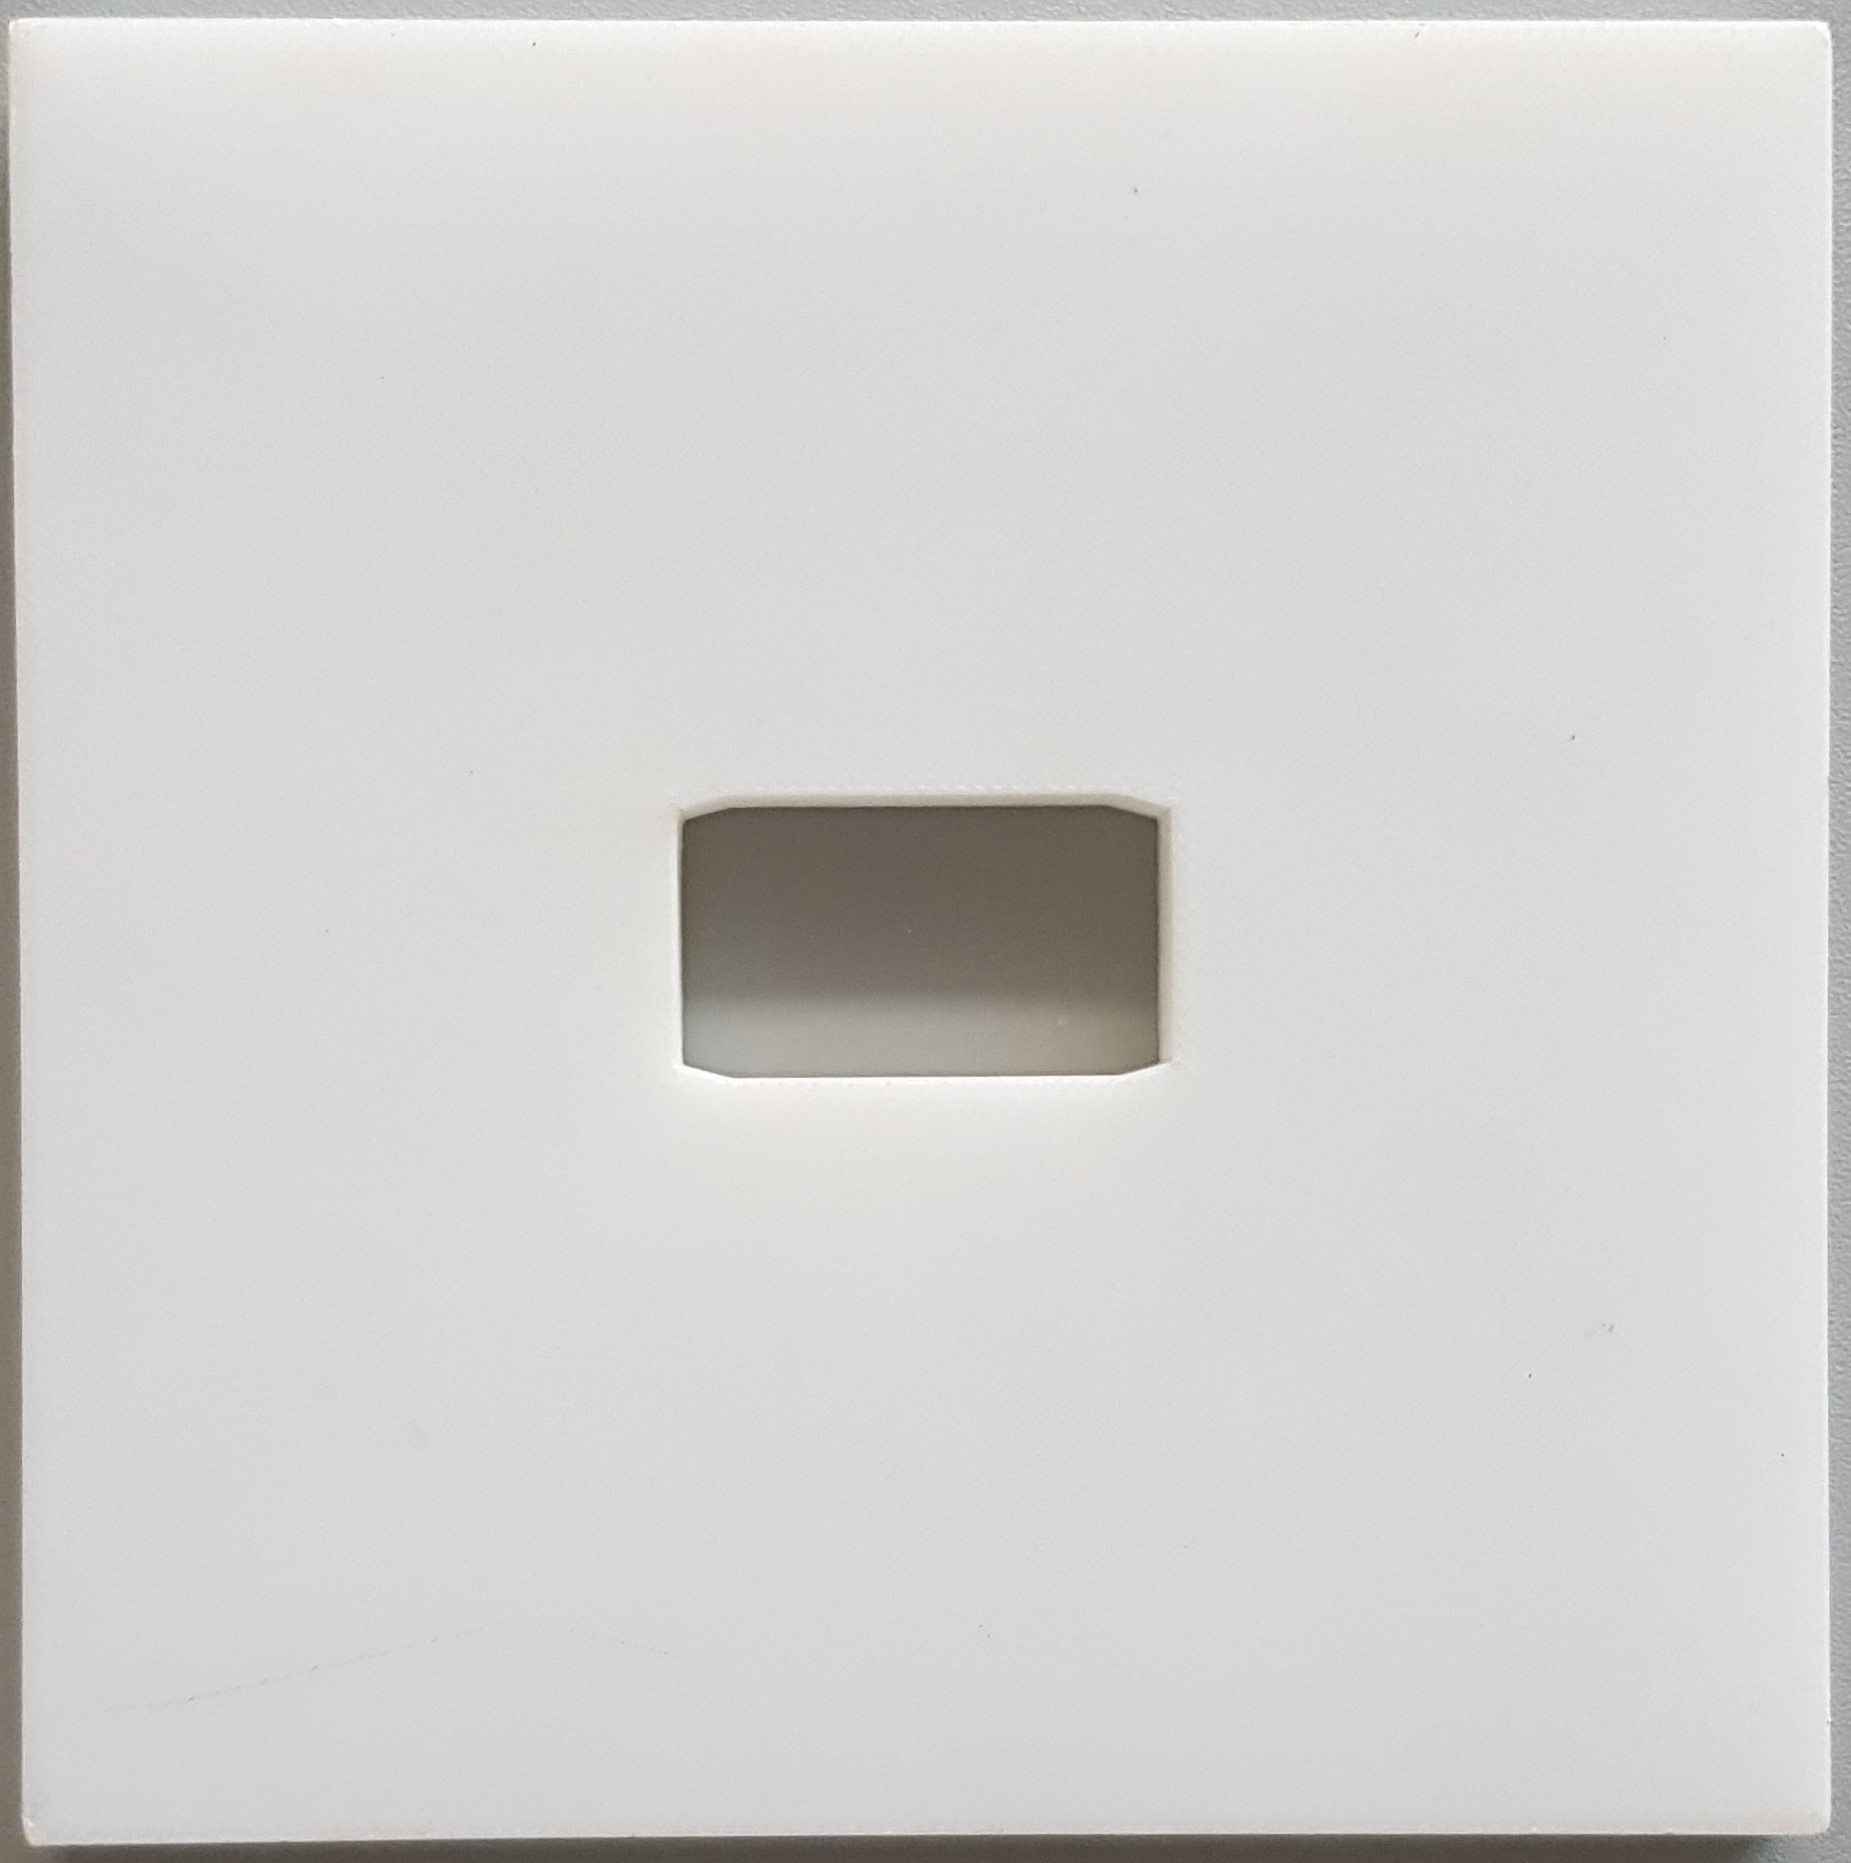
\includegraphics[width = 2.5 cm, height = 2.5 cm]{images/tile10.jpg}
\caption{Cavity tiles with two possible orientations}
\label{fig:twopossibility}
\end{minipage}
\end{figure}

\newpage

\item One tile has four possible orientation
\begin{figure}[h!]
\begin{minipage}{\textwidth}
\centering 
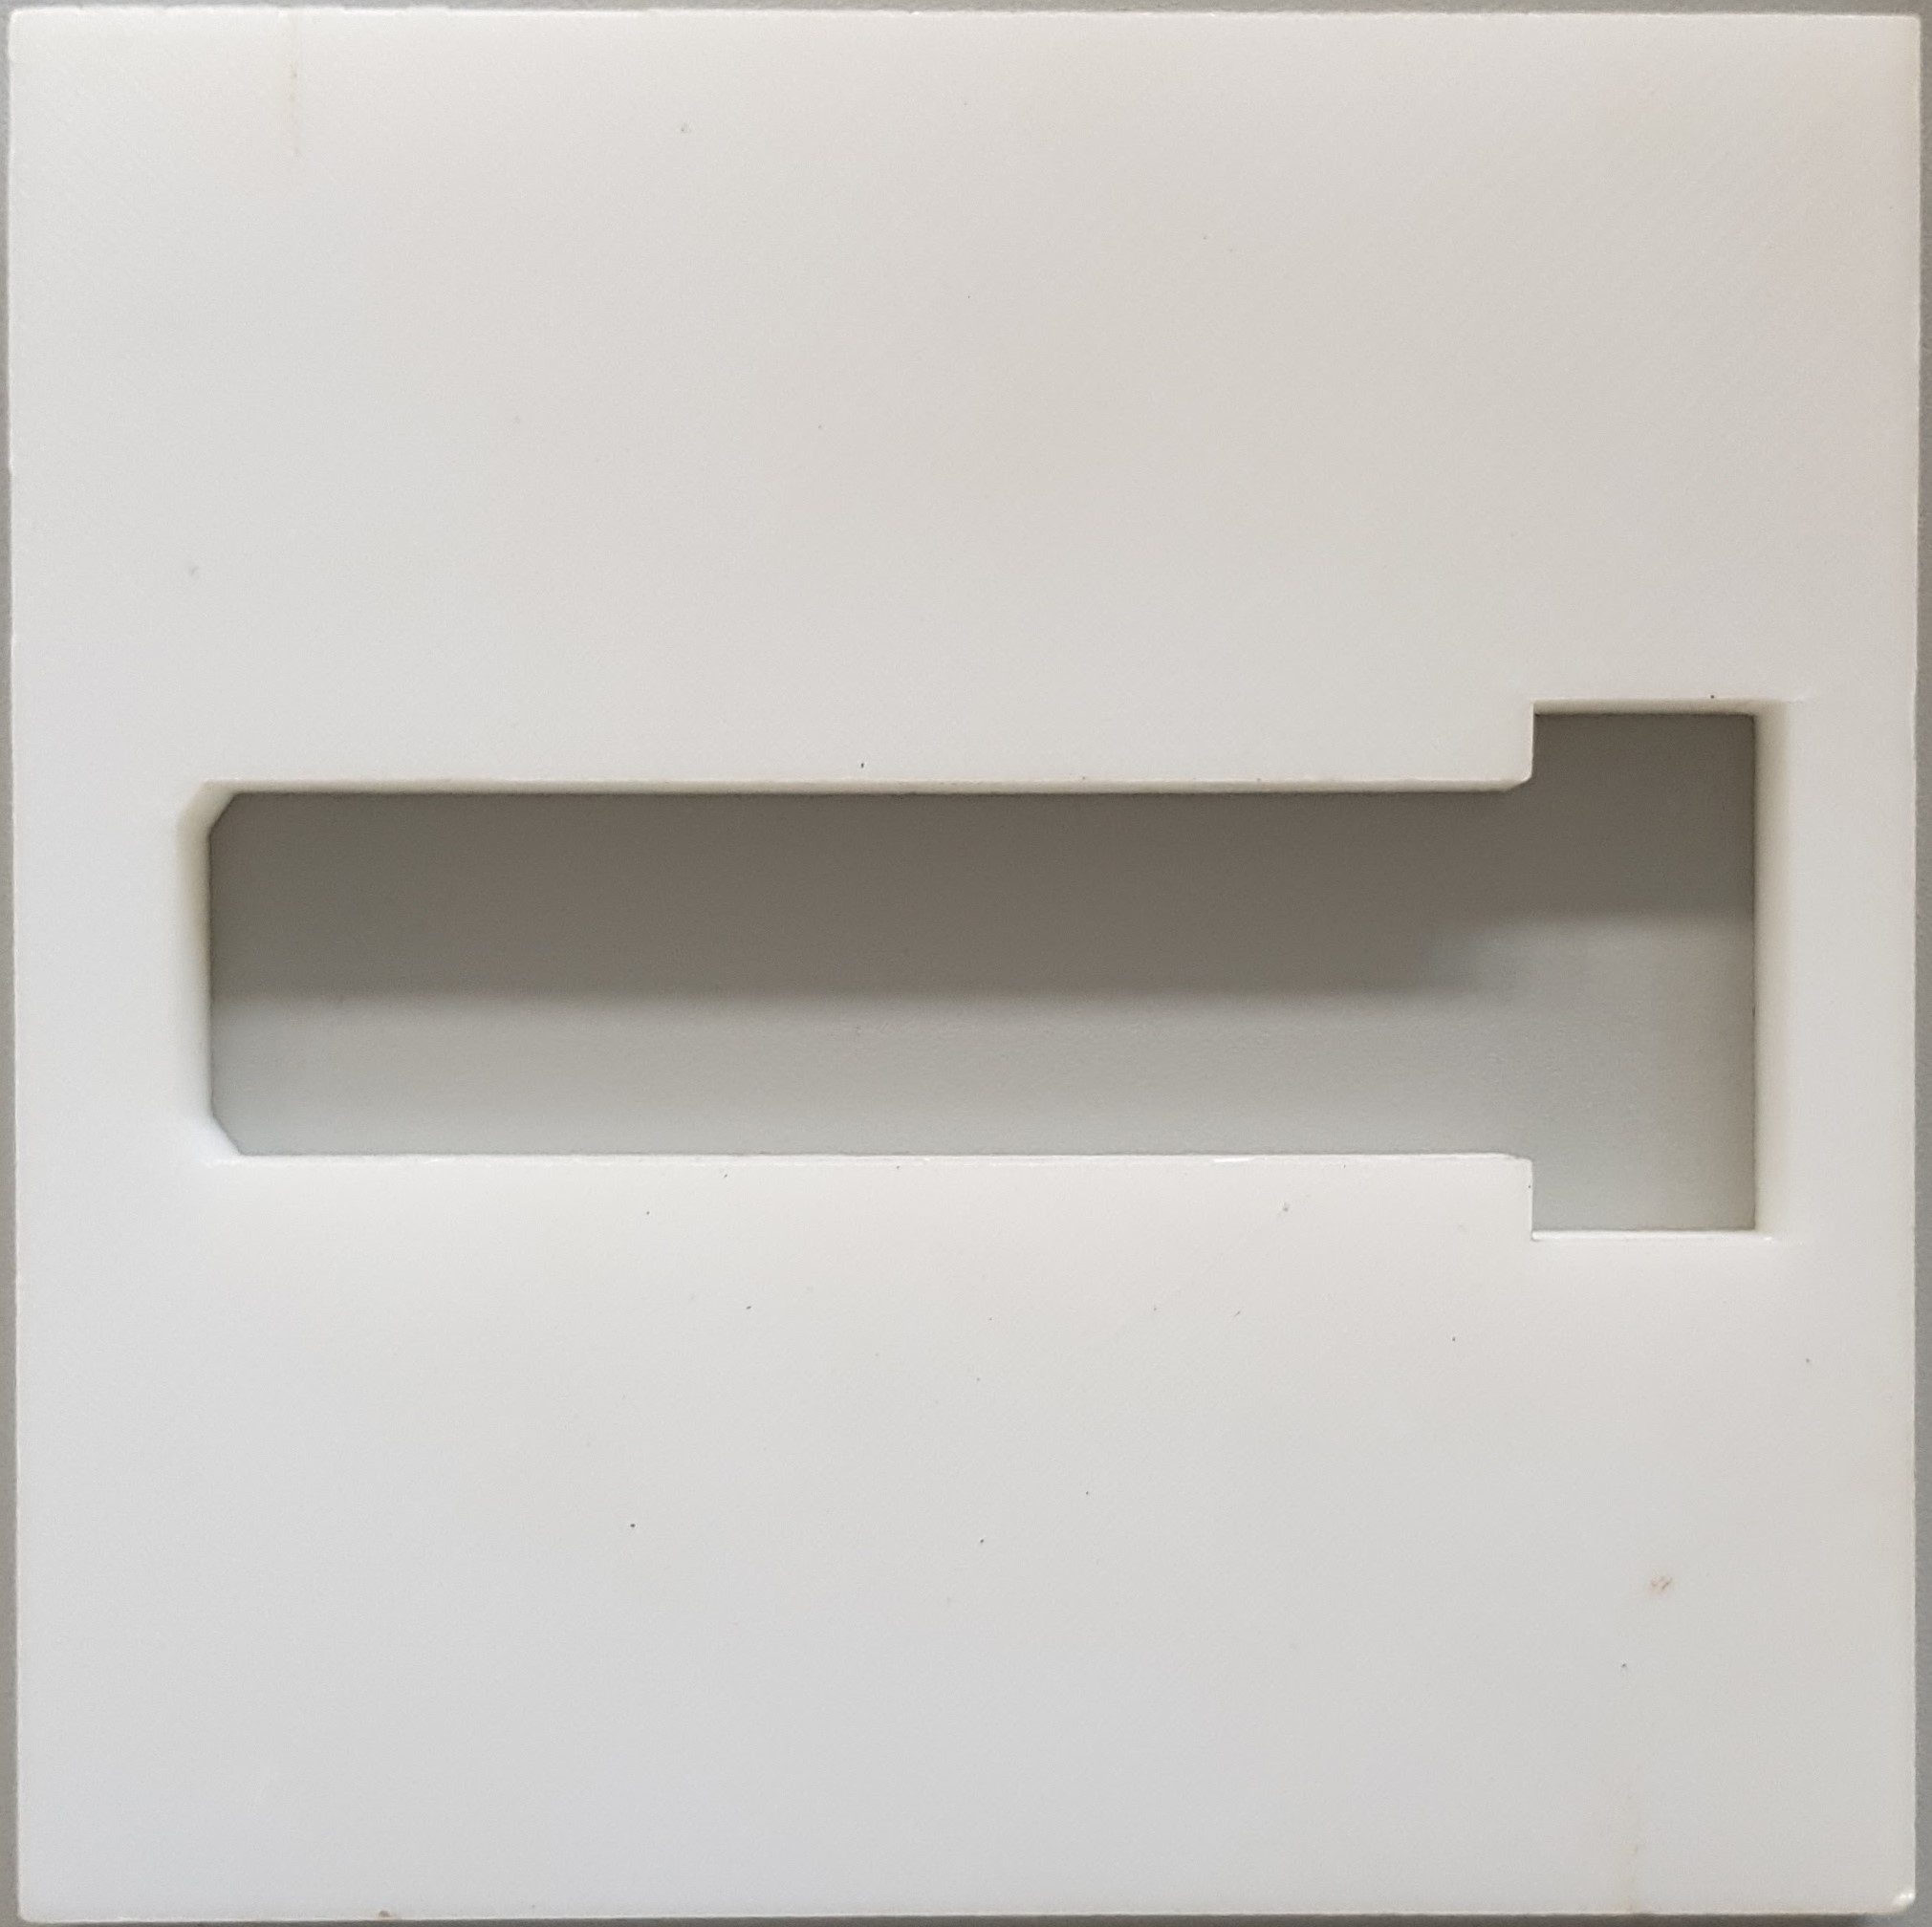
\includegraphics[width = 2.5 cm, height = 2.5 cm ]{images/tile11.jpg}
\caption{Single cavity tile with four possible orientations}
\end{minipage}
\end{figure}
\end{itemize}


\item Images of all cavity tiles in all possible orientations [total 19 images] are stored in the database
\item  The title for each stored image consist of the details of the object (that will fit in the cavity tile), object's orientation and cavity tile's orientation
\end{itemize}


\begin{minipage}[b]{0.35\linewidth}
\begin{center}
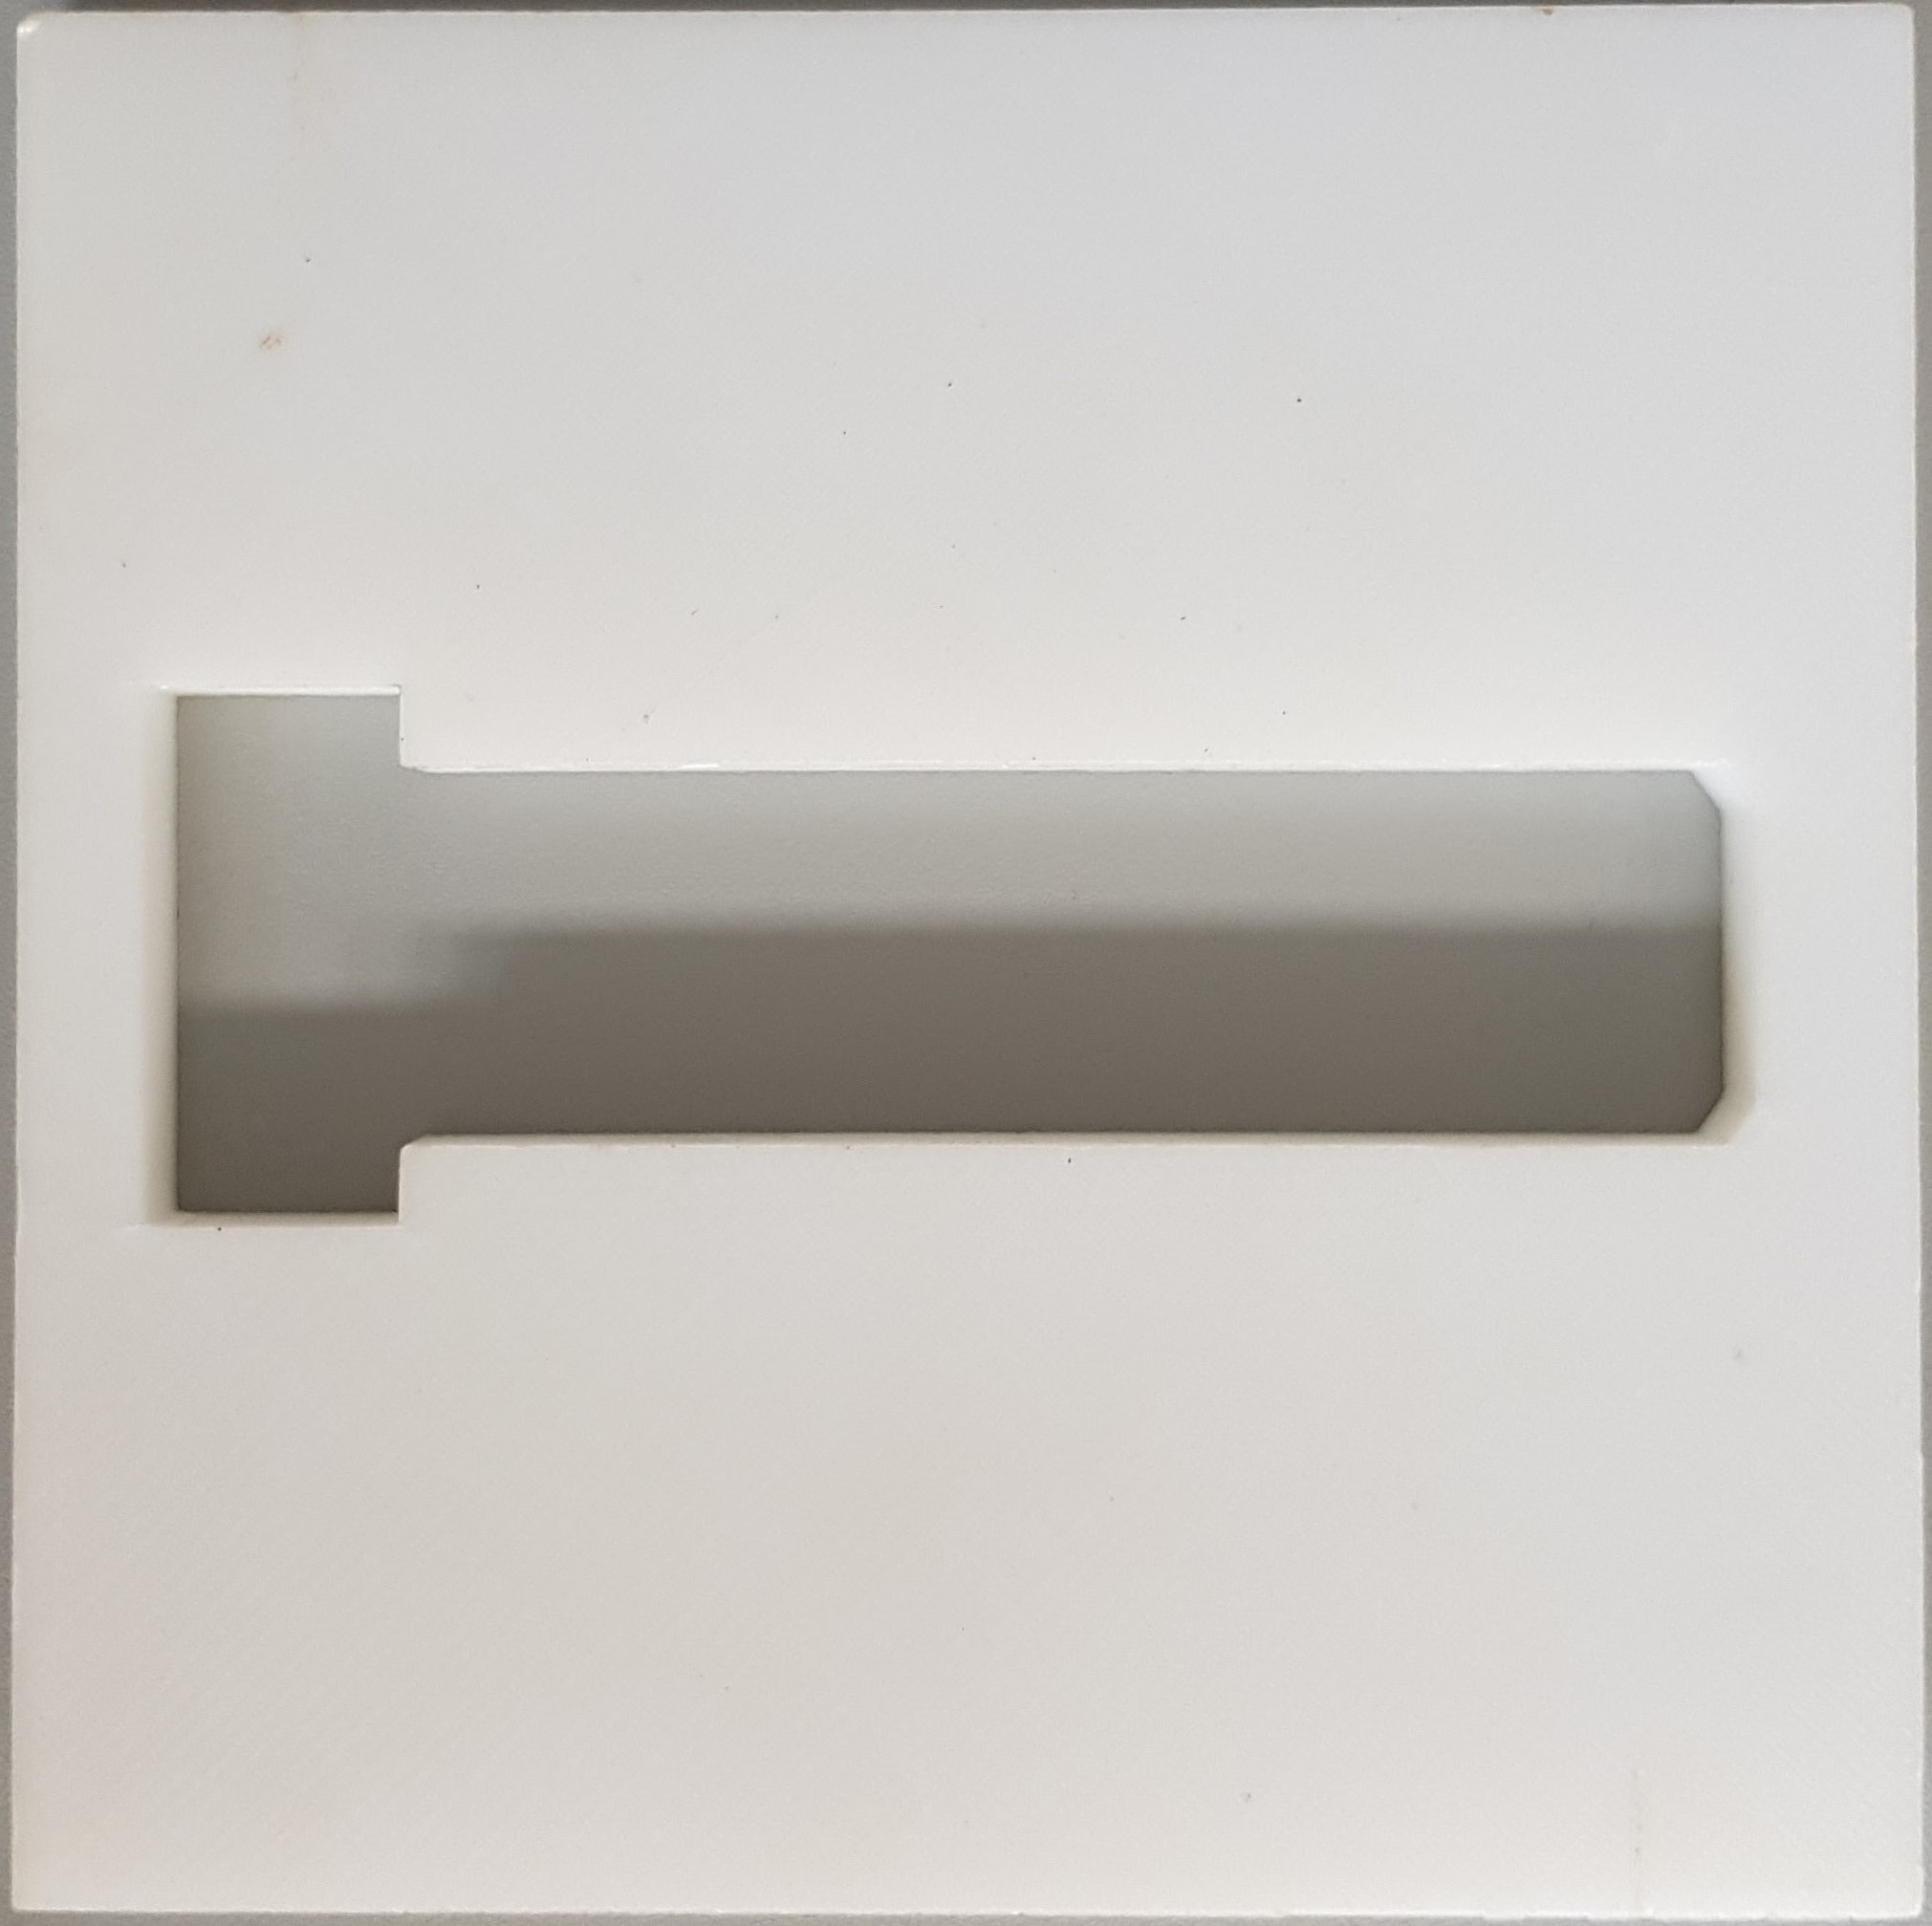
\includegraphics[height=5\baselineskip]{images/Screw_Horizontal_180.jpg}
\end{center}

\end{minipage}
\begin{minipage}[b]{0.65\linewidth}
\begin{flushleft}
Name: \textbf{Screw\_Horizontal\_270} \\ 
Meaning of the name: \\ 
Object that fits the cavity tile: \textbf{screw} \\
Orientation of the object: \textbf{Horizontal} \\
Orientation of the cavity tile:\textbf{ 180 degree}
\end{flushleft}

\end{minipage}



\begin{minipage}[b]{0.35\linewidth}

\begin{center}
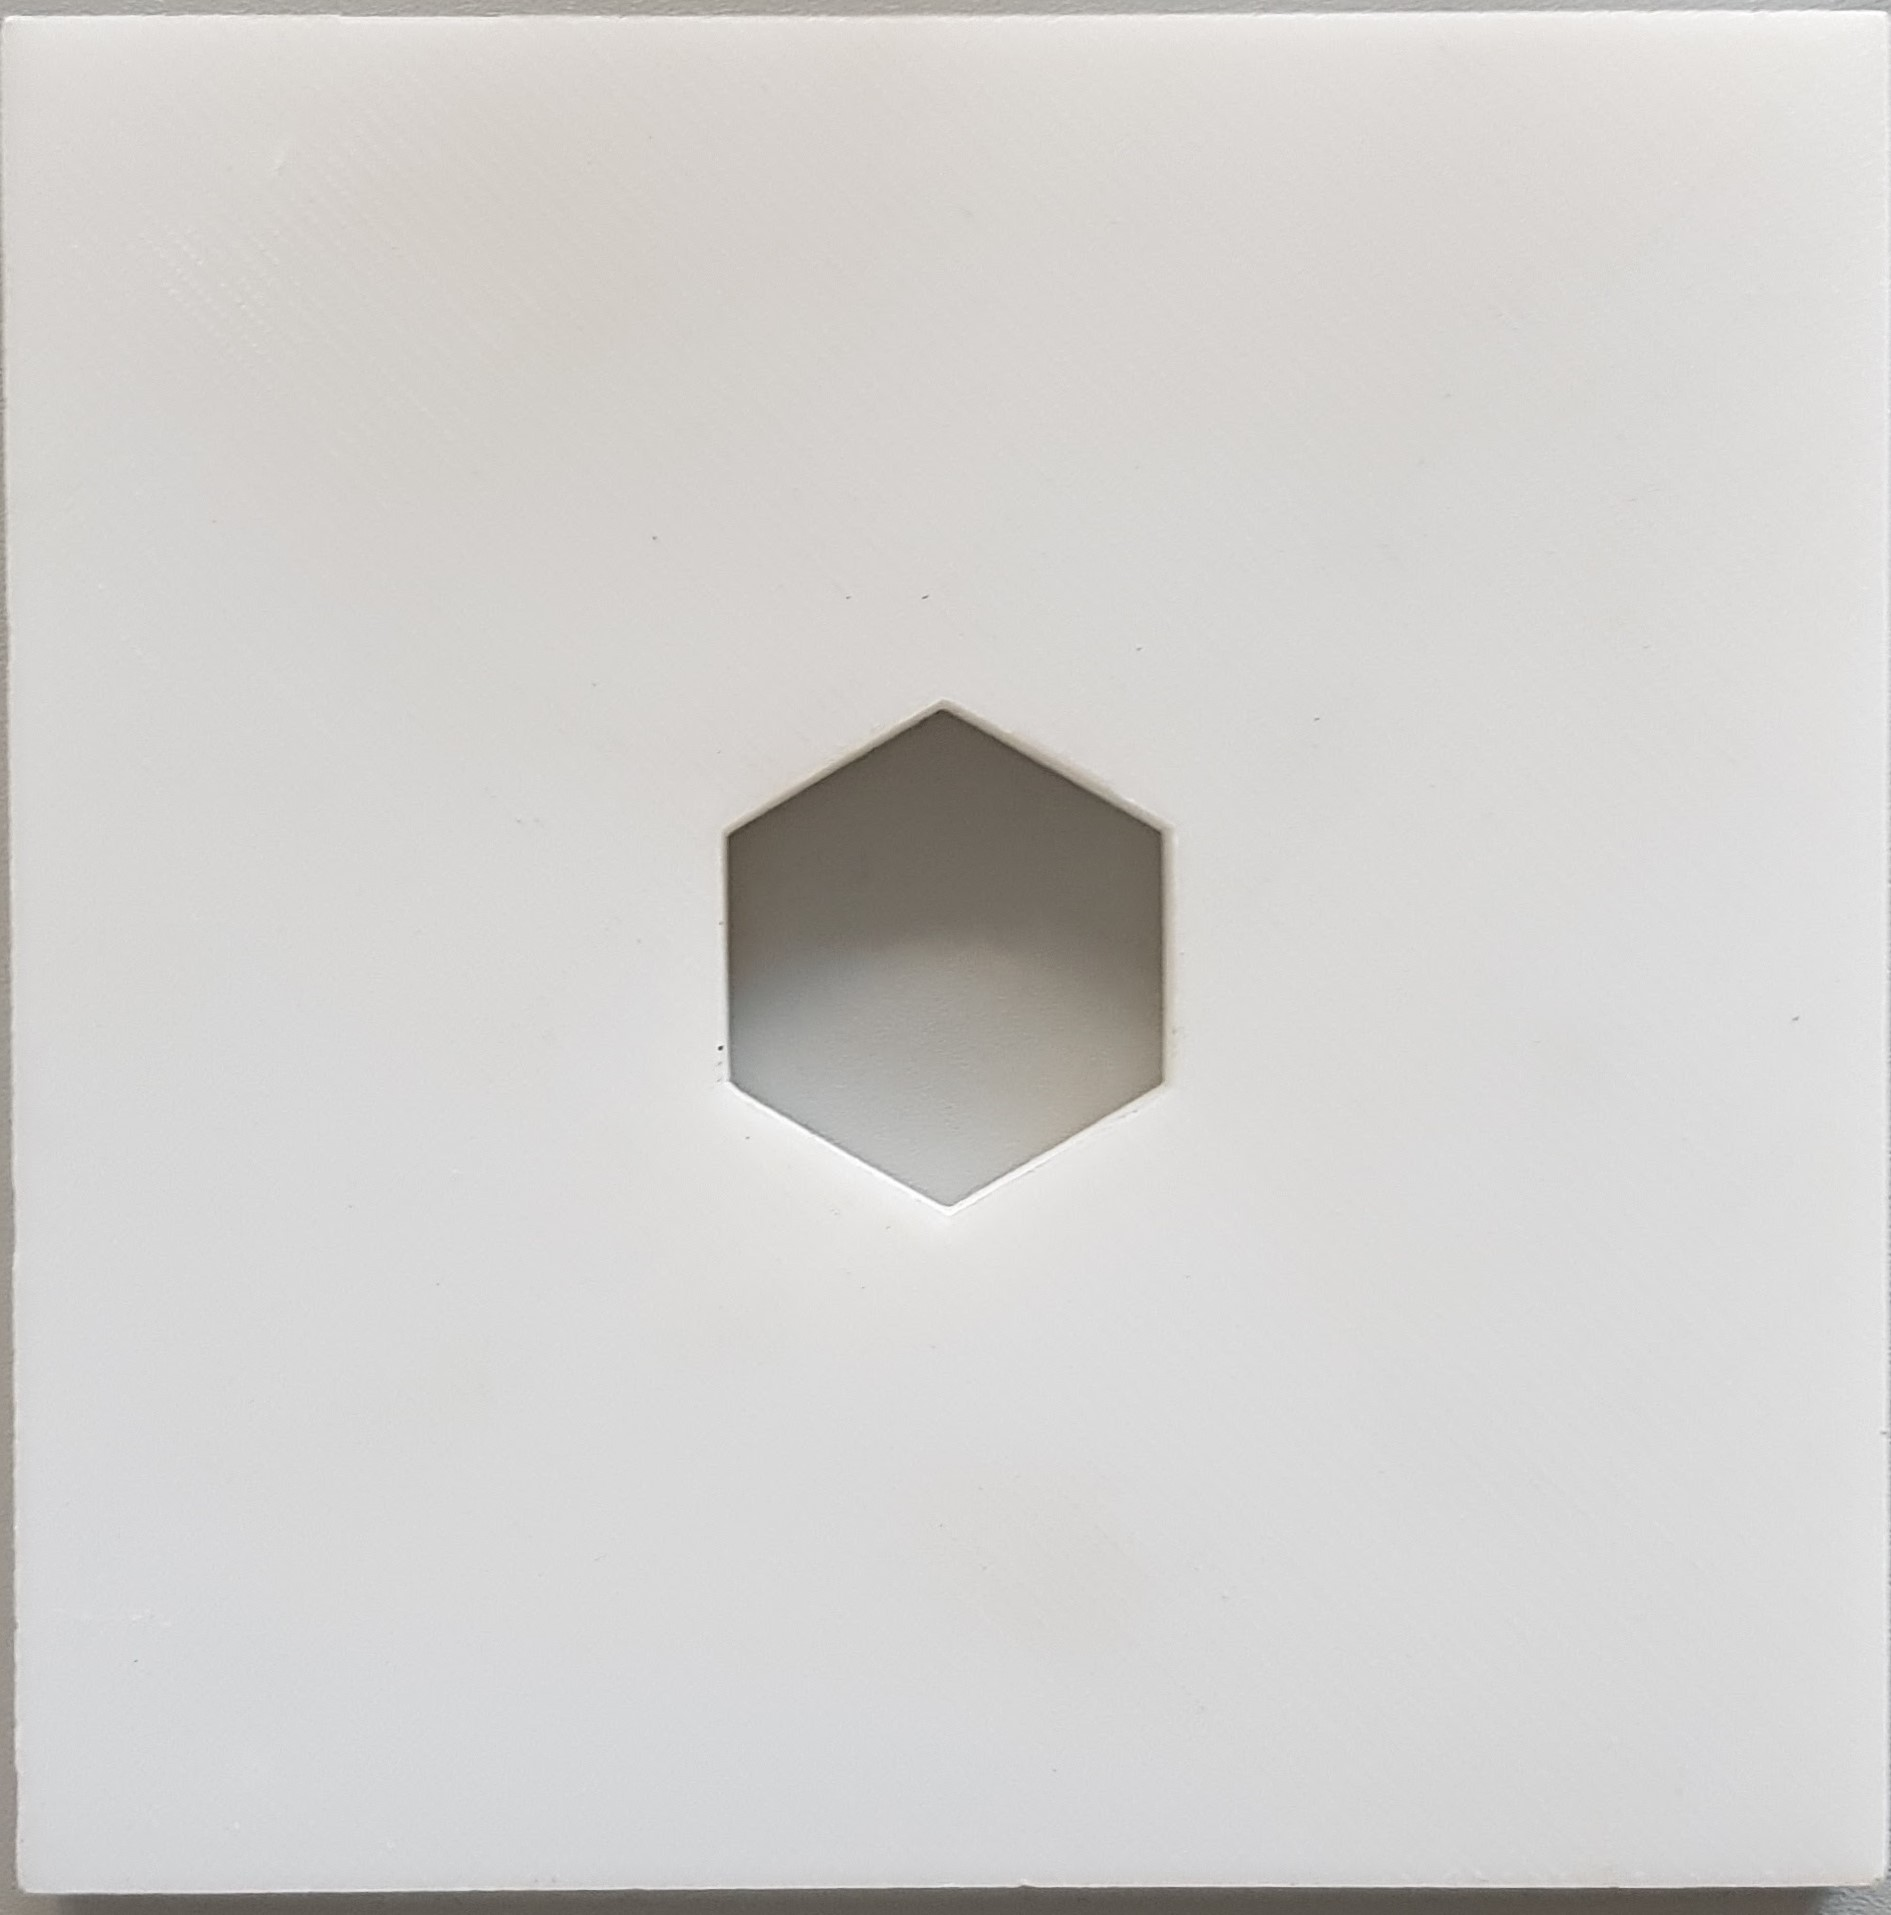
\includegraphics[height=5\baselineskip]  {images/SmallNut_Horizontal_00.jpg}
\end{center}

\end{minipage}
\begin{minipage}[b]{0.65\linewidth}
\begin{flushleft}
Name: \textbf{SmallNut\_Horizontal\_00} \\ 
Meaning of the name: \\ 
Object that fits the cavity tile: \textbf{SmallNut} \\
Orientation of the object: \textbf{Horizontal} \\
Orientation of the cavity tile:\textbf{ 0 degree}
\end{flushleft}

\end{minipage}

\begin{minipage}[b]{0.35\linewidth}

\begin{center}
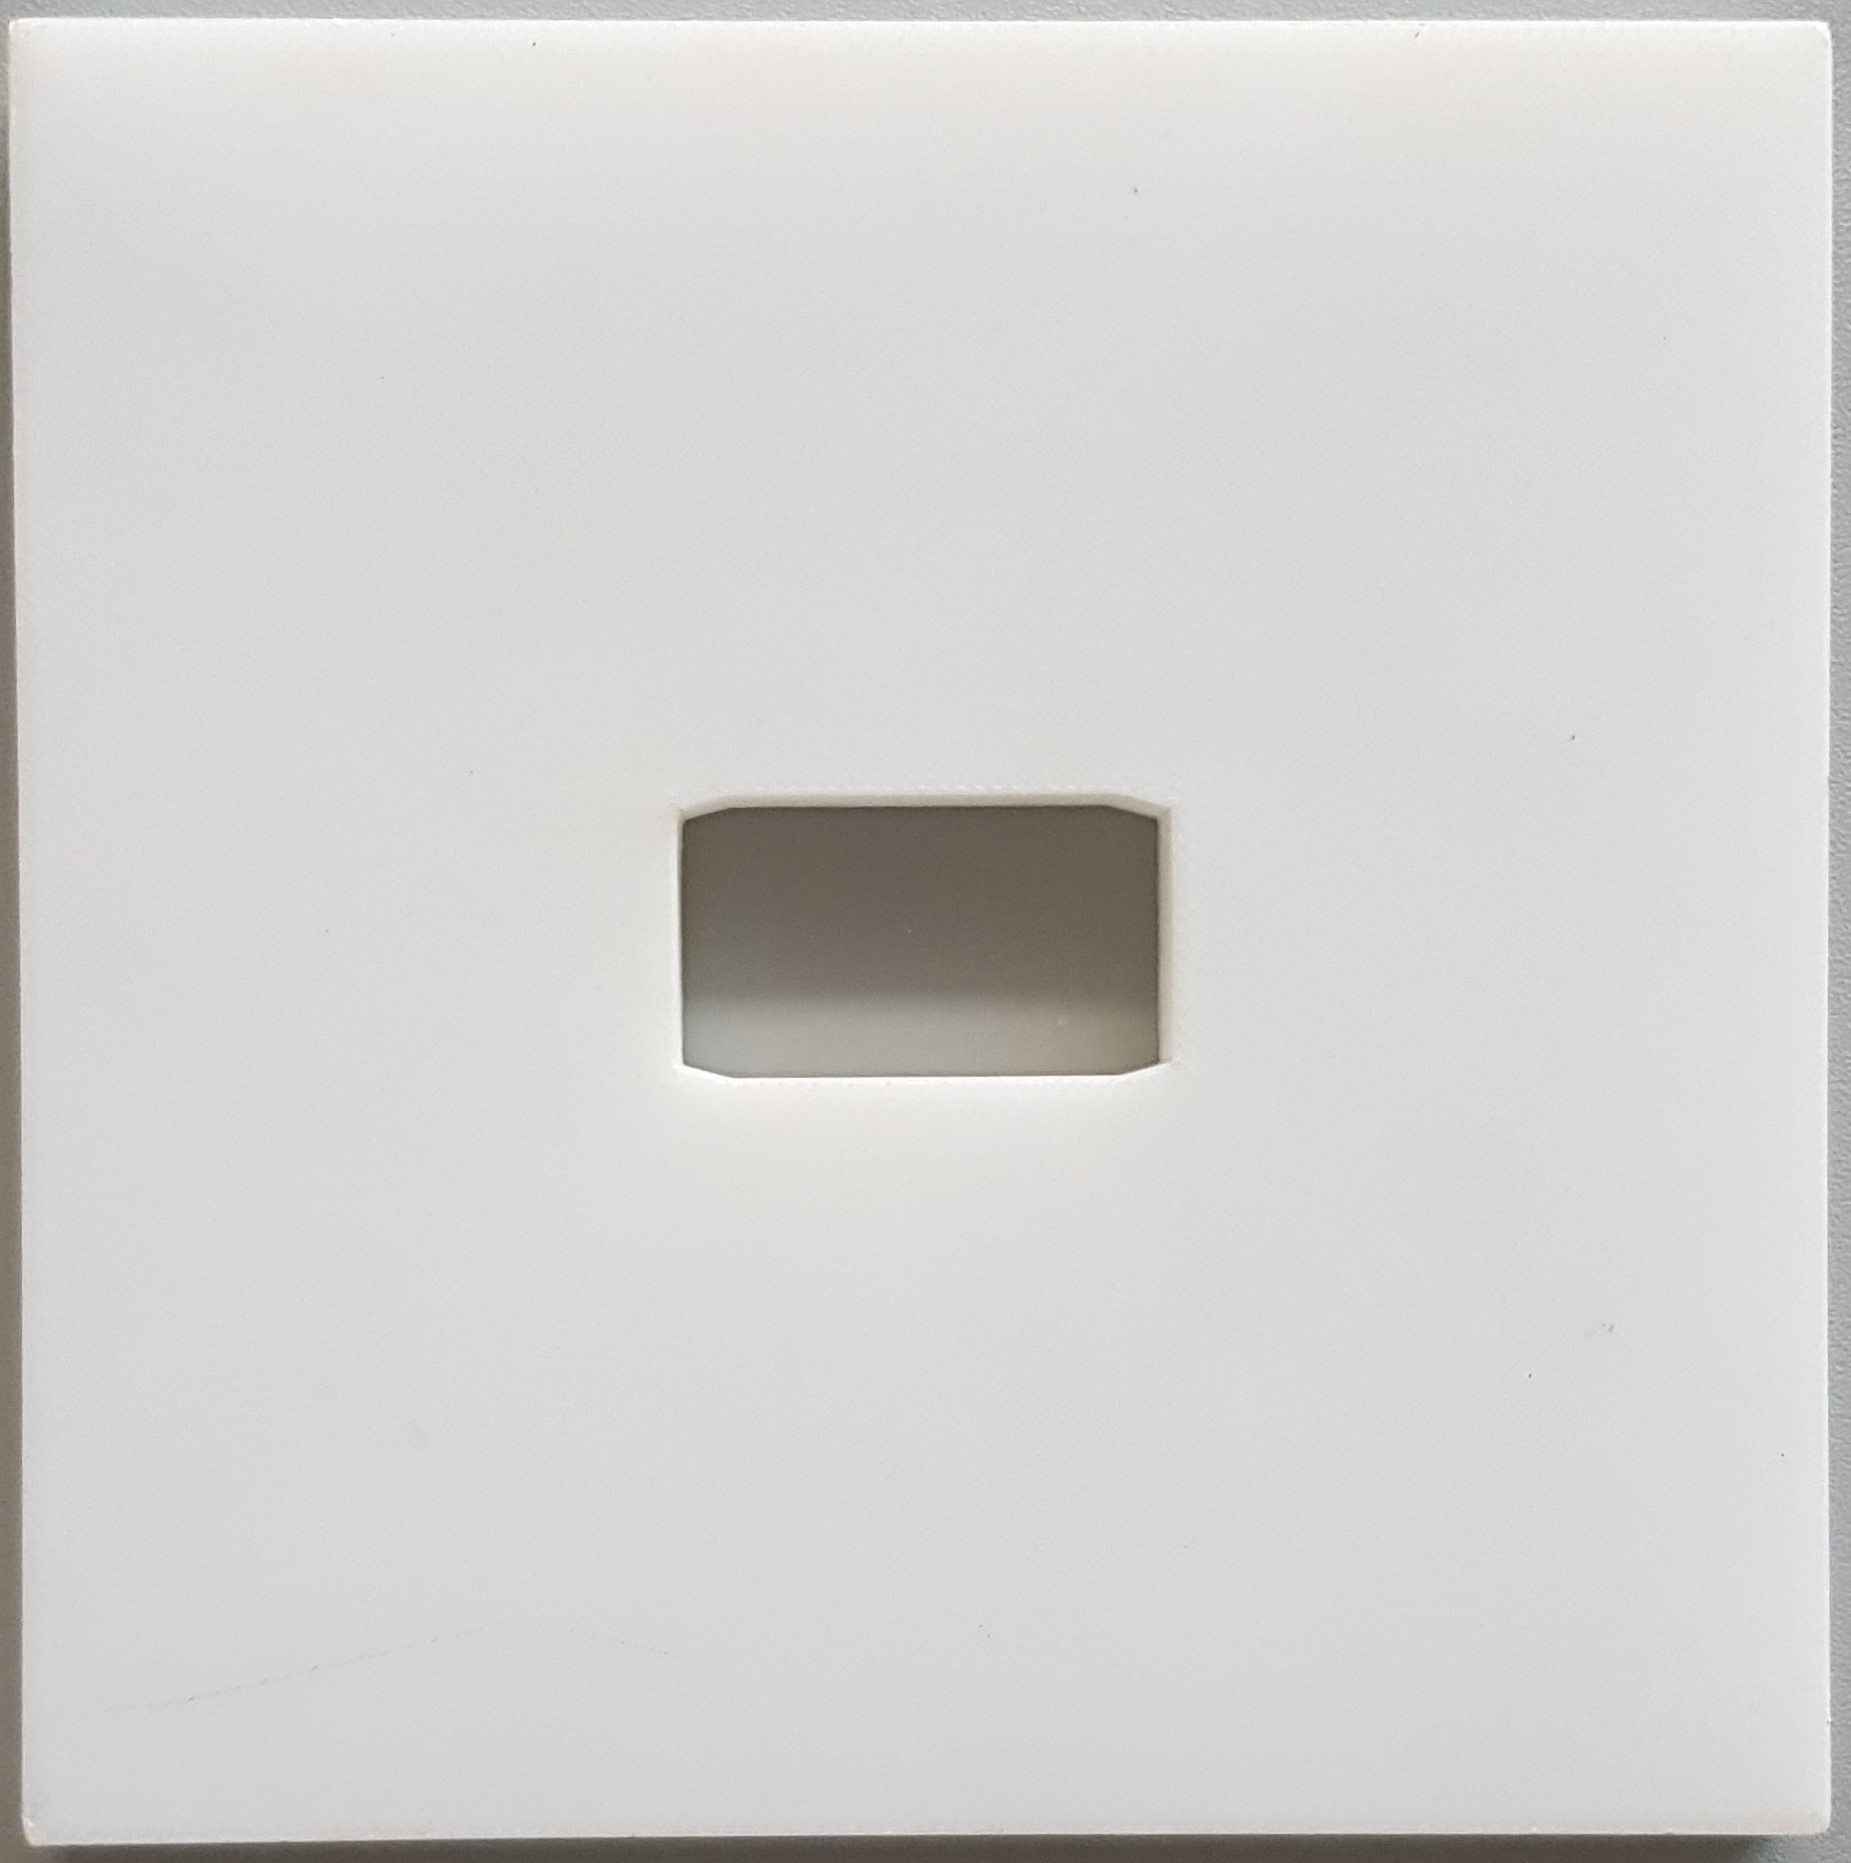
\includegraphics[height=5\baselineskip]{images/SmallNut_Vertical_00.jpg}
\end{center}

\end{minipage}
\begin{minipage}[b]{0.65\linewidth}
\begin{flushleft}
Name: \textbf{SmallNut\_Vertical\_0} \\ 
Meaning of the name: \\ 
Object that fits the cavity tile: \textbf{SmallNut} \\
Orientation of the object: \textbf{Vertical} \\
Orientation of the cavity tile:\textbf{ 0 degree}
\end{flushleft}

\end{minipage}



\subsubsection*{Mean Square Error(MSE)}
 The Mean Square Error (MSE) image comparison method is based on the formula: \\
 
 
 \begin{equation}
  MSE = \frac{1}{mn}   \sum^{m-1}_{i=0}  \sum^{n-1}_{j=0} [I(i,j) - K(i,j)] ^2
\end{equation}  
\begin{quote}
With I and K being the two compared images.
\end{quote}


In MSE, both images are converted into the same size. Then, the difference (error) between each pixel of both the images are taken and squared. The summation of all the error square will give the MSE value. 
The lower the error, the more similar are the images. 

There is another technique for image comparison called Structural Similarity Measure (SSM). 

\subsection*{Structurality Similarity Index Measure (SSIM)}

The SSIM models the changes in the structural information of the images. While MSE models the error. 

It is based on the formula \cite{third}
\begin{equation}
SSIM(x,y) = \frac{(2\mu_{x}\mu_{y}+C_{1})(2\sigma_{xy}+C_{2})}{(\mu^{2}_{x}+\mu^{2}_{y}+C_{1})(\sigma^{2}_{x}+\sigma^{2}_{y}+C_{1})}
\end{equation}
where, 
$\mu - mean $
$\sigma - variance $
$c - covariance $

This is used to compare two windows rather than two images \\ 
The output value ranges from -1 to 1, where 1 represents a perfect match

\begin{figure}[h!]

\centering 
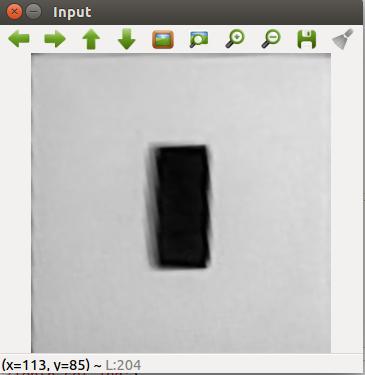
\includegraphics[scale = 0.3 ]{images/ComparisonInput.png}
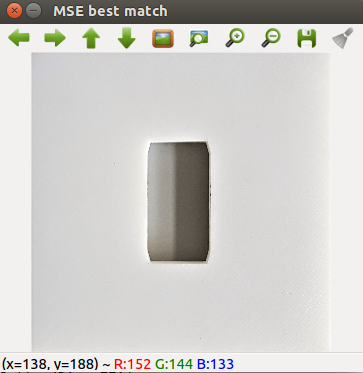
\includegraphics[scale = 0.3 ]{images/Comparison_MSE_BestMatch.png}
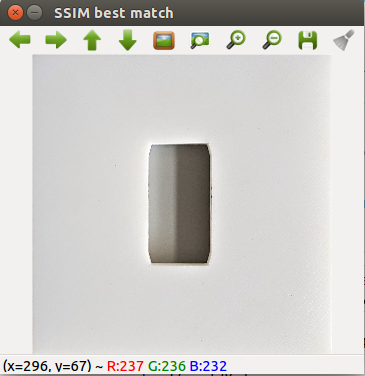
\includegraphics[scale = 0.3]{images/Comparison_SSIM_BestMatch.png}
\caption{From the left. First image shows the extracted tile image, that is given as an input to the MSE or SSIM comparison algorithm. The second image is the best match found in the database using MSE method. The third image shows the best match found using the SSIM method.}
\label{fig:Comparions_result}

\end{figure}

\subsection*{For better efficiency}
For the comparison techniques seen above perform well, the images are preprocessed:
\begin{itemize}
\item The image is converted into \textbf{gray scale}. 
\item Both images to be compared are \textbf{resized} to an equal size.
\item A \textbf{binary threshold} is applied to the image, in order to increase the contrast between cavity and tile, to normalize the colors of the images (get rid of shadows and non-homogeneous lighting), but mainly to provide a clear shape of the cavity (Fig:\ref{fig:Comparions_PreProcessing})
\item \textbf{Median blur} is applied to get rid of the salt and pepper noise (Fig:\ref{fig:Comparions_PreProcessing})
\end{itemize}
\begin{figure}[h!]
\begin{minipage}{\textwidth}
\centering 

\includegraphics[scale = 0.3]{images/AfterThreshholding.png}
\hspace{1cm}

\includegraphics[scale = 0.3 ]{images/AfterMedianBlur.png}
\caption{From the left.First, the image after applying a threshold. Second, after using the median blur.}
\label{fig:Comparions_PreProcessing}
\end{minipage}
\end{figure}

\subsubsection*{Optimisation:}

Not yet implemented

\paragraph*{When the difference between the best match and second best match is very low}

If in MSE the difference between the top two best matches is very low, then the SSIM result is considered.

\paragraph*{When best match of MSE and SSIM are different}

From the input image the contour is detected and the area is calculated. This area is compared with the area of the cavities calculated from the database cavity tiles. The best match by area comparison is used to decide on the database image.

\section{Evaluation and results}

\subsection{Used for evaluation}

\begin{itemize}
\item Eight images have been used for evaluation purpose (fig. \ref{fig:datasets}).
\item All images have the PPT platform in it but from different angles with different cavity tiles.
\item Five of the images show five tiles, placed in the PPT platform, with regular lighting, no occlusion and no other objects.
 \item The three remaining images have been created to test extreme conditions.
\item For the five regular images, some tiles have specifically been chosen to check whether the system is capable of differentiating the size, while the rest is selected arbitrarily.
\begin{enumerate}
\item The first image consists of simple shapes, where the focus is placed on differentiating between the same shape with a different size, which could give problems due to the similarity of the two shapes (fig. \ref{fig:datasets}, top, most left).
\item The second image is introducing more complex shapes, that could be harder to classify and recreate while using homography (fig. \ref{fig:datasets}, top, second from the left).
\item In the third image only small similar looking shapes have been chosen to test the algorithm for a number of similar shapes (fig. \ref{fig:datasets}, top, second from the right).
\item The fourth image shows four variations of the same 2 dimensional shape, that fit to different 3 dimensional objects (fig. \ref{fig:datasets}, top, most right).
\item The fifth image is used to determine how the algorithm works for similar shapes with different orientations (fig. \ref{fig:datasets}, bottom, most left).
\end{enumerate}
\item For the three remaining sets the focus is set to special conditions rather then testing the algorithm for the distinction between different shapes.
\begin{enumerate}

\item In the sixth image, the number of tiles has been reduced to four in order to test border cases (fig. \ref{fig:datasets}, bottom, second from the left), the algorithm is not expected to solve this problem, it is just an additional case.
\item The Seventh image shows images that correspond to a problem that occurs if other areas in the image have the same color and shape of the cavities (fig. \ref{fig:datasets}, bottom, second form the right).
\item In the last image, the light-source has been switched of to create a darker image (fig. \ref{fig:datasets}, bottom, most right).
\end{enumerate}
\item It can easily be seen, that each example image from the eight datasets has different areas of lighting, thus no dataset testing for shadows was necessary.
\end{itemize}

\begin{figure}[h!]
\begin{minipage}{\textwidth}
\centering
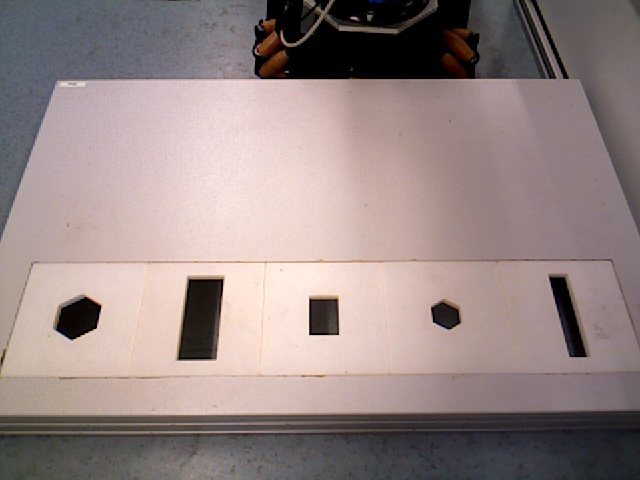
\includegraphics[scale=0.15]{images/First_set.jpg}\hspace{0.1cm}
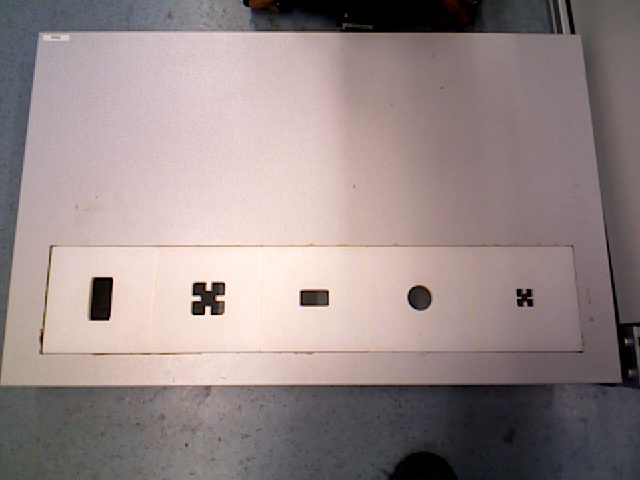
\includegraphics[scale=0.15]{images/Second_set.jpg}
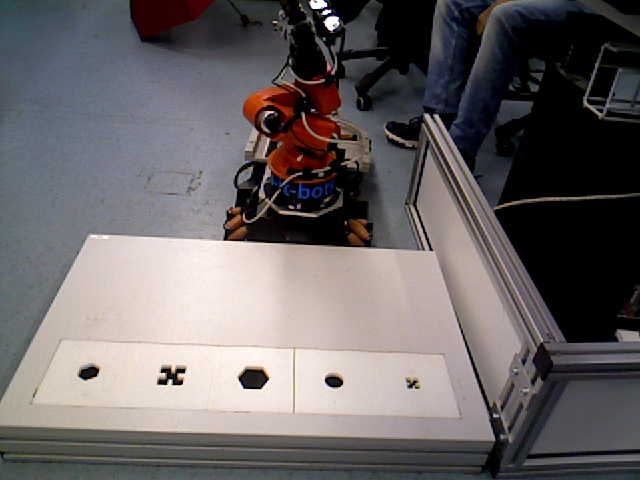
\includegraphics[scale=0.15]{images/Third_set.jpg}
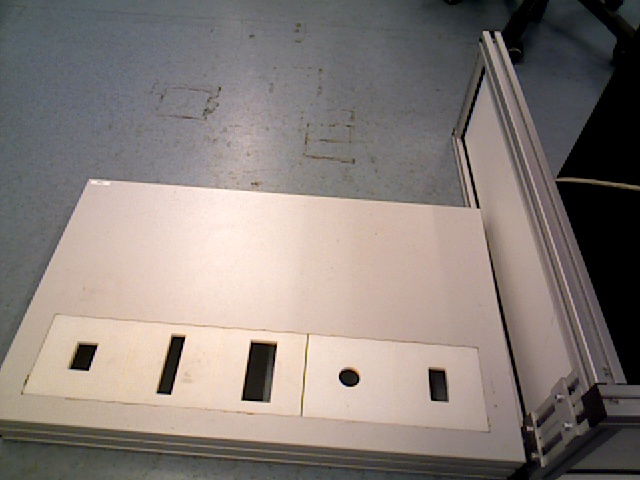
\includegraphics[scale=0.15]{images/Fourth_set.jpg}\vspace{0.1cm}
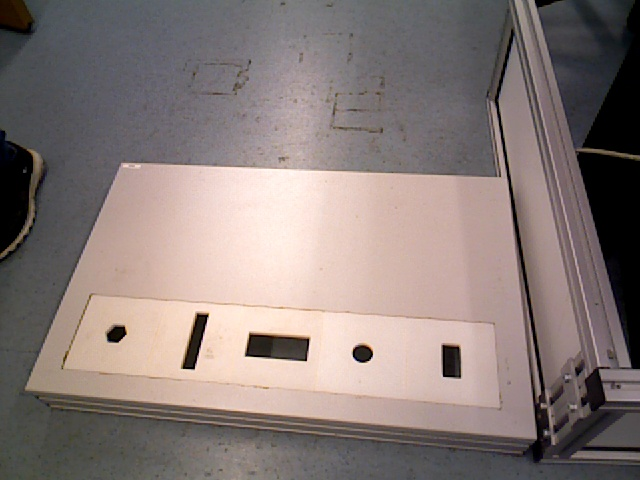
\includegraphics[scale=0.15]{images/Fifth_set.jpg}\hspace{0.1cm}
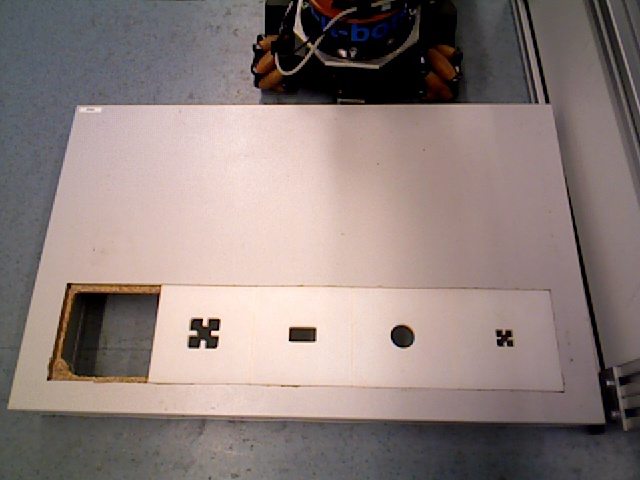
\includegraphics[scale=0.15]{images/Sixth_set.jpg}
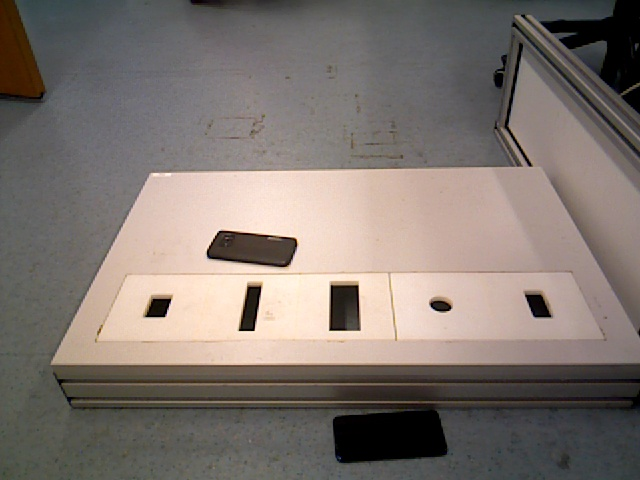
\includegraphics[scale=0.15]{images/Seventh_set.jpg}
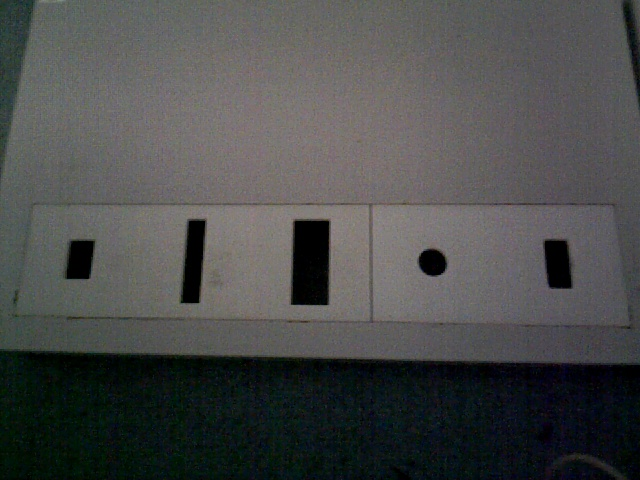
\includegraphics[scale=0.15]{images/Eigth_set.jpg}
\caption{Example images for the eight datasets, starting with one in the top left corner, to eight in the lower right.}
\label{fig:datasets}
\end{minipage}
\end{figure}

\section{Results}

\subsection{Results for normal cases}
\begin{tabular}{cccccc}
 \hline
 Operations & Image01 & Image02 & Image03 & Image04 & Image05 \\
 \hline
 Center of cavity detection & \checkmark & \checkmark & \checkmark & \checkmark & \checkmark \\
 Cropping 					& \checkmark & \checkmark & \checkmark & \checkmark & \checkmark \\
 Detecting the five tiles 	& \checkmark & \checkmark & \checkmark & \checkmark & \checkmark \\
 Detecting the corners		 & \checkmark & \checkmark & x & x & \checkmark \\
 Homography 						& \checkmark & \checkmark & x & x & \checkmark \\
 Number of cavity tiles extracted & 5 & 5 & 0 & 0 & 5 \\
 Number of objects matched 			& 5 & 5 & 0 & 0 & 4 \\
\end{tabular}

\paragraph{Summary}
\begin{itemize}
\item The algorithm is able to robustly detect the center of the cavity for all five tiles in the normal test cases
\item When there is a slight gap between the cavity tiles in the PPT platform, the contour detection finds two contours
\item Hence the corner detection also finds the corners of only one set of cavity tiles
\item The corner detection on the cropped image is not working correctly for each image
\item The comparison of images using MSE was able to find the correct match for 14 out of 15 tiles during the test run
\item When the clarity of the image is too poor the comparison technique fails
\item As shown in the Fig:\ref{fig:result}, the object for the first tile is supposed to be small nut, but the algorithm identifies it as a cylinder. This is because there is only a minimal difference between the hexagon and the circle.
\end{itemize}

\begin{figure}[h!]
\begin{minipage}{\textwidth}
\centering 
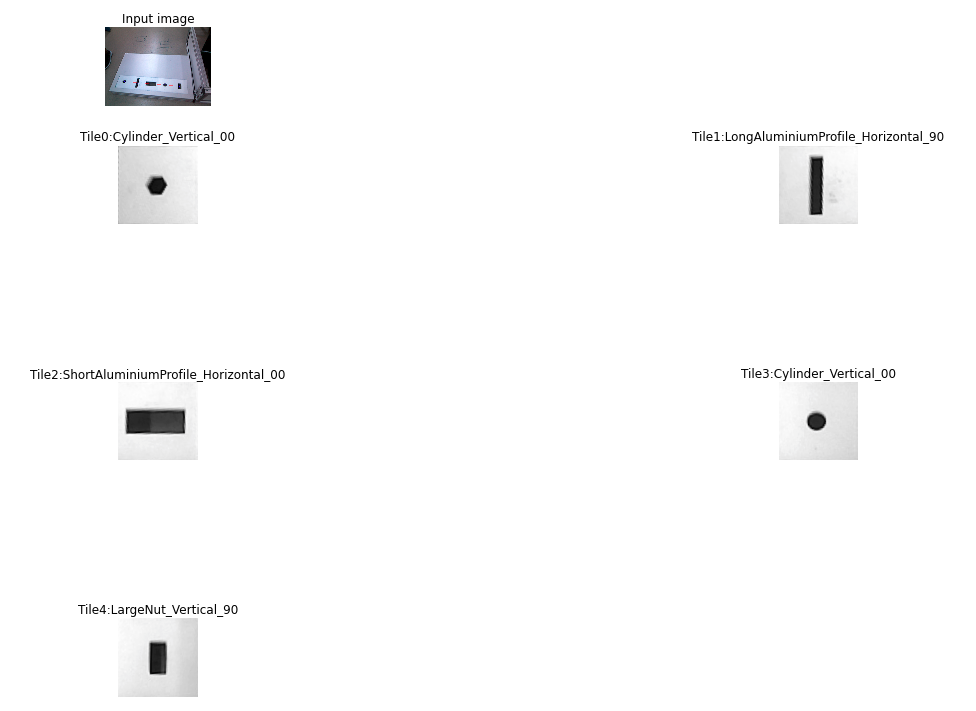
\includegraphics[scale = 0.5 ]{images/resultFrame06.png}
\caption{The results for the fifth image. The top left image shows the original input image. the 5 remaining images show one of the extracted tiles along with the identified object and orientation shown in the captions.}
\label{fig:result}
\end{minipage}
\end{figure}


\subsection{Results for special cases}
\begin{tabular}{cccc}
\hline
Operations & Image06 & Image07 & Image08 \\
Center of cavity detection & \checkmark & \checkmark & x \\
 Cropping 					& \checkmark & \checkmark & x \\
 Detecting the five tiles 	& x & \checkmark & x  \\
 Detecting the corners		 & x & x & x  \\
 Homography 						& x & x & x  \\
 Number of cavity tiles extracted & 0 & 0 & 0  \\
 Number of objects matched 			& 0 & 0 & 0  \\
\end{tabular}

\paragraph{Summary}
\begin{itemize}
\item The algorithm doesn't work properly on dark lighting
\end{itemize}

\section{Conclusion:}


\begin{thebibliography}{99}
	\bibitem{first} Robocup @work rulebook, p. 35. Robocup-rulebook2017
	\bibitem{second} Webpage, last viewed 13.12.17 20:25, https://docs.opencv.org/3.1.0/dc/da5/tutorial\_py\_drawing\_functions.html
	\bibitem{third} Comparing images with ssim and mse \\ https://www.pyimagesearch.com/2014/09/15/python-compare-two-images/
	\end{thebibliography}
\end{document}